%%%%%%%%%%%%%%%%%%%%%%%%%%%%%%%%%%%%%%%%%%%%%%%%%%%%%%%%%%%%%%%%%%%%%%%%%%%%%%%%
% title:
% authors:
%%%%%%%%%%%%%%%%%%%%%%%%%%%%%%%%%%%%%%%%%%%%%%%%%%%%%%%%%%%%%%%%%%%%%%%%%%%%%%%%
\def\fullver{0}
\def\submission{1}
\documentclass[11pt]{article}

\usepackage[letterpaper,hmargin=1in,vmargin=1in]{geometry}
\usepackage[backref=true,backend=bibtex]{biblatex}

\DefineBibliographyStrings{english}{%
  backrefpage = {page},% originally "cited on page"
  backrefpages = {pages},% originally "cited on pages"
}


\usepackage{framed}
%\usepackage{cite}
\usepackage[hidelinks]{hyperref}

\usepackage{color}
\usepackage{float}
\usepackage{setspace}
\usepackage{booktabs}
\usepackage{outlines}
\usepackage{enumitem}
\usepackage{epsfig}
\usepackage{wrapfig}
\usepackage{textcomp}
\usepackage{rotating}
\usepackage{xspace}
\usepackage{tikz}
\usetikzlibrary{calc,arrows,arrows.meta,shapes,positioning,matrix,decorations.pathreplacing}
\usepackage{amsthm}
\usepackage{amssymb}
\usepackage{pifont}
\usepackage{amsfonts}
\usepackage{amsmath}
\DeclareMathOperator*{\argmax}{arg\,max}
\DeclareMathOperator*{\argmin}{arg\,min}
\usepackage{cleveref}
\usepackage{bm}
\usepackage{listings}
\usepackage{mathtools}
\allowdisplaybreaks[2]
\usepackage{latexsym}
\usepackage{graphics}
\usepackage{graphicx}
\usepackage{fancyhdr}
\usepackage{url}
%\usepackage{enumerate}
\usepackage{adjustbox}
\usepackage{multirow}
\usepackage[font=small]{caption}
\usepackage[font=small]{subcaption}
\def\authnotes{1}
\newtheorem{thm}{Theorem} %[section]
\newtheorem*{theorem*}{Theorem}
\newtheorem{lem}{Lemma}
\newtheorem*{lemma*}{Lemma}

\newtheorem{cor}[thm]{Corollary}
\newtheorem{propo}[thm]{Proposition}
\newtheorem{defn}[thm]{Definition}
\newtheorem{assm}[thm]{Assumption}
\newtheorem{clm}[thm]{Claim}
\newtheorem{rem}[thm]{Remark}
\newtheorem{exa}{Example}
\newtheorem{fact}{Fact}

\newenvironment{theorem}{\begin{thm}
    \begin{sl}
    }%
    {
    \end{sl}
  \end{thm}}

\newenvironment{lemma}{\begin{lem}\begin{sl}}%
    {\end{sl}\end{lem}}
\newenvironment{corollary}{\begin{cor}\begin{sl}}%
    {\end{sl}\end{cor}}
\newenvironment{proposition}{\begin{propo}\begin{sl}}%
    {\end{sl}\end{propo}}
\newenvironment{definition}{\begin{defn}\begin{sl}}%
    {\end{sl}\end{defn}}
\newenvironment{assumption}{\begin{assm}\begin{em}}%
    {\end{em}\end{assm}}
\newenvironment{claim}{\begin{clm}\begin{sl}}%
    {\end{sl}\end{clm}}
\newenvironment{remark}{\begin{rem}\begin{em}}%
    {\end{em}\end{rem}}
\newenvironment{example}{\begin{exa}\begin{em}}%
    {\end{em}\end{exa}}

\newcommand{\lemautorefname}{Lemma}
\newcommand{\algorithmautorefname}{Algorithm}
\renewcommand{\subsectionautorefname}{Section}


% Deluxe proof enviroment
\iffalse
    \def\qsym{\vrule width0.6ex height1em depth0ex}
    \def\qedsym{{\hspace{5pt}\rule[-1pt]{3pt}{9pt}}}
    \newcount\proofqeded
    \newcount\proofended
    \def\qed{%\qedsym
    \end{rm}\addtolength{\parskip}{-0pt}
    \setlength{\parindent}{\saveparindent}
    \global\advance\proofqeded by 1 }
    \newenvironment{proof}%
     {\proofstart}%
     {\ifnum\proofqeded=\proofended\qed\fi \global\advance\proofended by 1
      \medskip}
    \makeatletter
    \def\proofstart{\@ifnextchar[{\@oprf}{\@nprf}}
    \def\@oprf[#1]{\begin{rm}\protect\vspace{6pt}\noindent{\bf Proof of #1:\
    }%
    \addtolength{\parskip}{5pt}\setlength{\parindent}{0pt}}
    \def\@nprf{\begin{rm}\protect\vspace{6pt}\noindent{\bf Proof:\ }%
    \addtolength{\parskip}{5pt}\setlength{\parindent}{0pt}}
  \makeatother
\fi


% Extra padding for table entries
\newcommand\Tvsp{\rule{0pt}{2.6ex}}
\newcommand\Bvsp{\rule[-1.2ex]{0pt}{0pt}}
\newcommand{\TabPad}{\hspace*{5pt}}
\newcommand\TabSep{@{\hspace{5pt}}|@{\hspace{5pt}}}
\newcommand\TabSepLeft{|@{\hspace{5pt}}}
\newcommand\TabSepRight{@{\hspace{5pt}}|}



%\def\qedsym{{\ifnum\llncsclass=0  \else {\hspace{5pt}\rule[-1pt]{3pt}{9pt}} \fi}}
\def\qedsym{{\hspace{5pt}\rule[-1pt]{3pt}{9pt}} }

\def\pseudocodesize{ \footnotesize }

\renewcommand{\arraystretch}{1.3}
\DeclareMathAlphabet{\mathsl}{OT1}{cmr}{m}{sl}
\DeclareMathAlphabet{\mathsc}{OT1}{cmr}{m}{sc}


% Reference expansions
\newcommand{\secref}[1]{\mbox{Section~\ref{#1}}}
\newcommand{\subsecref}[1]{\mbox{Subsection~\ref{#1}}}
\newcommand{\apref}[1]{\mbox{Appendix~\ref{#1}}}
\newcommand{\thref}[1]{\mbox{Theorem~\ref{#1}}}
\newcommand{\thmrefshort}[1]{\mbox{\textbf{Th~\ref{#1}}}}
\newcommand{\exref}[1]{\mbox{Example~\ref{#1}}}
\newcommand{\defref}[1]{\mbox{Definition~\ref{#1}}}
\newcommand{\corref}[1]{\mbox{Corollary~\ref{#1}}}
\newcommand{\lemref}[1]{\mbox{Lemma~\ref{#1}}}
\newcommand{\clref}[1]{\mbox{Claim~\ref{#1}}}
\newcommand{\propref}[1]{\mbox{Proposition~\ref{#1}}}
\newcommand{\consref}[1]{\mbox{Construction~\ref{#1}}}
\newcommand{\figref}[1]{\mbox{Figure~\ref{#1}}}
%\newcommand{\eqref}[1]{\mbox{Equation~\ref{#1}}}

\newcommand{\enumref}[1]{\mbox{(\ref{#1})}}

\newcommand{\thmlabel}[1]{\textnormal{\textbf{[#1]}}}

\newcommand{\SetFigFont}[5]{} % This is for xfig issue
\newcommand{\SetFigFontNFSS}[5]{} % This is for xfig issue

\DeclarePairedDelimiter{\ceil}{\lceil}{\rceil}%
\DeclarePairedDelimiter{\floor}{\lfloor}{\rfloor}%
\DeclarePairedDelimiter\absv{\lvert}{\rvert}%
%\DeclarePairedDelimiter\norm{\lVert}{\rVert}%
\DeclarePairedDelimiter\prns{(}{)}%
\DeclarePairedDelimiter\braces{\{}{\}}%
\DeclarePairedDelimiter\bracks{[}{]}%
\DeclarePairedDelimiterX\condprns[2]{(}{)}{\,#1 \;\delimsize\vert\; #2\,}
\DeclarePairedDelimiterX\condbrks[2]{[}{]}{\,#1 \;\delimsize\vert\; #2\,}
\DeclarePairedDelimiterX\condbraces[2]{\{}{\}}{\,#1 \;\delimsize\vert\; #2\,}

% ========================================================================

% Lists

\newcounter{ctr}
\newcounter{savectr}
\newcounter{ectr}

\newlength{\saveparindent}
\setlength{\saveparindent}{\parindent}
\newlength{\saveparskip}
\setlength{\saveparskip}{\parskip}


\newenvironment{newitemize}{%
\begin{list}{\mbox{}\hspace{5pt}$\bullet$\hfill}{\labelwidth=15pt%
\labelsep=5pt \leftmargin=20pt \topsep=3pt%
\setlength{\listparindent}{\saveparindent}%
\setlength{\parsep}{\saveparskip}%
\setlength{\itemsep}{3pt} }}{\end{list}}


\newenvironment{newenum}{%
\begin{list}{{\rm (\arabic{ctr})}\hfill}{\usecounter{ctr} \labelwidth=17pt%
\labelsep=5pt \leftmargin=22pt \topsep=3pt%
\setlength{\listparindent}{\saveparindent}%
\setlength{\parsep}{\saveparskip}%
\setlength{\itemsep}{2pt} }}{\end{list}}

\newenvironment{tiret}{%
\begin{list}{\hspace{2pt}\rule[0.5ex]{6pt}{1pt}\hfill}{\labelwidth=15pt%
\labelsep=3pt \leftmargin=22pt \topsep=3pt%
\setlength{\listparindent}{\saveparindent}%
\setlength{\parsep}{\saveparskip}%
\setlength{\itemsep}{2pt}}}{\end{list}}


\newenvironment{blocklist}{\begin{list}{}{\labelwidth=0pt%
\labelsep=0pt \leftmargin=0pt \topsep=10pt%
\setlength{\listparindent}{\saveparindent}%
\setlength{\parsep}{\saveparskip}%
\setlength{\itemsep}{20pt}}}{\end{list}}

\newenvironment{blocklistindented}{\begin{list}{}{\labelwidth=0pt%
\labelsep=30pt \leftmargin=30pt\topsep=5pt%
\setlength{\listparindent}{\saveparindent}%
\setlength{\parsep}{\saveparskip}%
\setlength{\itemsep}{10pt}}}{\end{list}}

\newenvironment{onelist}{%
\begin{list}{{\rm (\arabic{ctr})}\hfill}{\usecounter{ctr} \labelwidth=18pt%
\labelsep=7pt \leftmargin=25pt \topsep=2pt%
\setlength{\listparindent}{\saveparindent}%
\setlength{\parsep}{\saveparskip}%
\setlength{\itemsep}{2pt} }}{\end{list}}

\newenvironment{twolist}{%
\begin{list}{{\rm (\arabic{ctr}.\arabic{ectr})}%
\hfill}{\usecounter{ectr} \labelwidth=26pt%
\labelsep=7pt \leftmargin=33pt \topsep=2pt%
\setlength{\listparindent}{\saveparindent}%
\setlength{\parsep}{\saveparskip}%
\setlength{\itemsep}{2pt} }}{\end{list}}

\newenvironment{centerlist}{%
\begin{list}{\mbox{}}{\labelwidth=0pt%
\labelsep=0pt \leftmargin=0pt \topsep=10pt%
\setlength{\listparindent}{\saveparindent}%
\setlength{\parsep}{\saveparskip}%
\setlength{\itemsep}{10pt} }}{\end{list}}

\newenvironment{newcenter}[1]{\begin{centerlist}\centering%
\item #1}{\end{centerlist}}

\newenvironment{codecenter}[1]{\begin{small}\begin{centerlist}\centering%
\item #1}{\end{centerlist}\end{small}}

% =========================================================================

% Math

\newlength{\savejot}
\setlength{\jot}{3pt}
\setlength{\savejot}{\jot}

\newenvironment{newmath}{\begin{displaymath}%
\setlength{\abovedisplayskip}{4pt}%
\setlength{\belowdisplayskip}{4pt}%
\setlength{\abovedisplayshortskip}{6pt}%
\setlength{\belowdisplayshortskip}{6pt} }{\end{displaymath}}

\newenvironment{newequation}{\begin{equation}%
\setlength{\abovedisplayskip}{4pt}%
\setlength{\belowdisplayskip}{4pt}%
\setlength{\abovedisplayshortskip}{6pt}%
\setlength{\belowdisplayshortskip}{6pt} }{\end{equation}}

%\newcommand{\headingg}[1]{{\textbf{#1}}}
%\newcommand{\heading}[1]{{\vspace{6pt}\noindent\textbf{#1}}}
\newcommand{\ind}{\hspace*{1.5em}}
\newcommand{\indsm}{\hspace*{.75em}}
\newcommand{\indeqn}{\;\;\;\;\;\;\;}
\newcommand{\bits}{\{0,1\}}
\newcommand{\zon}[1]{\bits^{#1}}
\newcommand{\emptystring}{\varepsilon}
\newcommand{\xor}{{\:\oplus\:}}
%\newcommand{\concat}{\,,\,}
\newcommand{\smidge}{{\kern .05em}}
\newcommand{\Colon}{{\smidge\colon\smidge}}
\newcommand{\norm}[1]{\|#1\|}
\def\poly{\mathop{\rm poly}\nolimits}
\def\div{\mathop{\rm div}\nolimits}
%\newcommand{\ro}{RO}
\newcommand{\advA}{{\mathcal A}}
\newcommand{\advB}{{\mathcal B}}
\newcommand{\advC}{{\mathcal C}}
\newcommand{\advD}{{\mathcal D}}
\newcommand{\advE}{{\mathcal E}}

\newcommand{\calA}{{\cal A}}
\newcommand{\calB}{{\cal B}}
\newcommand{\calC}{{\cal C}}
\newcommand{\calE}{{\cal E}}
\newcommand{\calF}{{\cal F}}
\newcommand{\calG}{{\cal G}}
\newcommand{\calH}{{\cal H}}
\newcommand{\calI}{{\cal I}}
\newcommand{\calJ}{{\cal J}}
\newcommand{\calO}{{\cal O}}
\newcommand{\calR}{{\cal R}}
\newcommand{\calS}{{\cal S}}
\newcommand{\calD}{{\cal D}}
\newcommand{\calK}{{\cal K}}
\newcommand{\calL}{{\cal L}}
\newcommand{\calM}{{\cal M}}
\newcommand{\calN}{{\cal N}}
\newcommand{\calP}{{\cal P}}
\newcommand{\calQ}{{\cal Q}}
\newcommand{\calT}{{\cal T}}
\newcommand{\calU}{{\cal U}}
\newcommand{\calV}{{\cal V}}
\newcommand{\calW}{{\cal W}}
\newcommand{\calX}{{\cal X}}
\newcommand{\calY}{{\cal Y}}

\newcommand{\N}{{{\mathbb N}}}
\newcommand{\Z}{{{\mathbb Z}}}
\newcommand{\G}{{{\textnormal G}}}
\newcommand{\Hgame}{{{\textnormal H}}}
\newcommand{\bigO}{\calO}
\newcommand{\goesto}{{\rightarrow}}
\newcommand{\eqdef}{\stackrel{\rm def}{=}}
\newcommand{\negsmidge}{{\hspace{-0.1ex}}}
\newcommand{\cdotsm}{\negsmidge\negsmidge\negsmidge\cdot\negsmidge\negsmidge\negsmidge}
\def\union{\cup}
\def\sep{\,}
\def\bigunion{\bigcup}
\def\suchthatt{\: :\:}
%\def\next{\hspace{12pt};\hspace{12pt}}
\def\nextt{\hspace{3pt};\hspace{6pt}}
\newcommand{\set}[2]{\{\:#1 \suchthatt #2\:\}}
\newcommand{\card}[1]{|#1|}
\def\leqq{\;\leq\;}
\def\eqq{\;=\;}
\def\geqq{\;\geq\;}
\def\lst{\;<\;}
\def\gst{\;>\;}
\def\prn#1{\left(#1\right)}

% \newcolumntype{y}[1]{%
% >{\hspace{0pt}}p{#1}}%

% \newcolumntype{x}[1]{%
% >{\centering\hspace{0pt}}p{#1}}%




\newcommand{\verylongleftarrow}[1]
      {\setlength{\unitlength}{.01in}
      \begin{picture}(#1,1) \put(#1,0){\vector(-1,0){#1}} \end{picture}}
\newcommand{\verylongrightarrow}[1]             %longleft and rightgoing arrows
      {\setlength{\unitlength}{.01in}           %for protocols
      \begin{picture}(#1,1) \put(0,0){\vector(1,0){#1}} \end{picture}}
\newcommand{\verylongbotharrow}[2]             %longleft and rightgoing arrows
      {\setlength{\unitlength}{.01in}           %for protocols
      \begin{picture}(#2,1) \put(#1,0){\vector(1,0){#1}}
                            \put(#1,0){\vector(-1,0){#1}} \end{picture}}
\newcommand{\leftgoing}[2]{{\stackrel{{\displaystyle #2}} {\verylongleftarrow{#1}}}}
\newcommand{\rightgoing}[2]{{\stackrel{{\displaystyle #2}} {\verylongrightarrow{#1}}}}
\newcommand{\bothgoing}[3]{{\stackrel{{\displaystyle #3}} {\verylongbotharrow{#1}{#2}}}}


\newcommand{\leftgoinga}[1]{\leftgoing{230}{#1} }
\newcommand{\rightgoinga}[1]{\rightgoing{230}{#1} }

\newcommand{\leftgoingb}[1]{\leftgoing{300}{#1} }
\newcommand{\rightgoingb}[1]{\rightgoing{300}{#1} }




\newcommand{\veryshortleftarrow}[1]
      {\setlength{\unitlength}{.01in}
      \begin{picture}(#1,1) \put(#1,0){\vector(-1,0){#1}} \end{picture}}


\newcommand{\getparse}[1]{{\:\stackrel{\raisebox{-0.5em}{{\hspace{0.1em}\mbox{\boldmath$\scriptscriptstyle
            #1$}}}}{\leftarrow}\:}}
\newcommand{\getu}{{\:\stackrel{\raisebox{-0.5em}{{\hspace{0.1em}\mbox{\boldmath$\scriptscriptstyle \cup$}}}}{\leftarrow}\:}}
\newcommand{\getdiff}{{\:\stackrel{{\scriptscriptstyle\hspace{0.2em} /}}{\leftarrow}\:}}
\newcommand{\getsr}{{\:{\leftarrow{\hspace*{-3pt}\raisebox{.75pt}{$\scriptscriptstyle\$$}}}\:}}
\newcommand{\get}[1]{{\:\leftarrow_{#1}\:}}
%\newcommand{\getsr}{{\:{\raisebox{3pt}{\veryshortleftarrow{15}}{\raisebox{1pt}{$\scriptscriptstyle\$$}}}\:}}
%\newcommand{\getsr}{{\:{\xleftarrow{\scriptscriptstyle\$}}\:}}
%\newcommand{\getsr}{{\:\stackrel{\raisebox{-0.5em}{$\scriptscriptstyle \hspace{0.2em}\$$}}{\leftarrow}\:}}
\newcommand{\sendsr}{{\:\stackrel{\scriptscriptstyle \hspace{0.2em}\$}{\rightarrow}\:}}
\renewcommand{\choose}[2]{{{#1}\atopwithdelims(){#2}}}
\newcommand{\abs}[1]{{\displaystyle \left| {#1} \right| }}
\newcommand{\E}{{\mbox{\bf E}}}
\newcommand{\EE}[1]{{\E\left[{#1}\right]}}
\newcommand{\EEE}[2]{{\E_{#1}\left[{#2}\right]}}
\newcommand{\Ex}{{\textbf E}}
\newcommand{\Exx}[1]{{\Ex\left[{#1}\right]}}
\newcommand{\Exxx}[2]{{\Ex_{#1}\left[{#2}\right]}}
\newcommand{\Var}{{\textnormal{Var}}}
\newcommand{\Varr}[1]{{\Var\left[{#1}\right]}}
\newcommand{\Varrr}[2]{{\Var_{#1}\left[{#2}\right]}}
\newcommand{\Prob}[1]{\Pr\left[\: #1 \:\right]}
\newcommand{\CondProb}[2]{{\Pr}\left[\: #1\:\left|\right.\:#2\:\right]}
\newcommand{\CondProbb}[3]{{\Pr}_{#1}\left[\: #2\:\left|\right.\:#3\:\right]}
\newcommand{\ProbExp}[2]{\Pr\left[\: #1 \: : \: #2\: \right]}
\newcommand{\Probb}[2]{{\Pr}_{#1}\left[\: #2 \:\right]}
\newcommand{\Probc}[2]{\Pr\left[\: #1 \:{\left|\right.}\:#2\:\right]}
\newcommand{\Probcc}[3]{{\Pr}_{#1}\left[\: #2 \:\left|\right.\:#3\:\right]}
\newcommand{\suchthat}{{\mbox{s.t.\ }}}
\newcommand{\qquadd}{{\quad}}
\def\d{{\delta}}
\def\e{{\epsilon}}
\newcommand{\ceiling}[1]{\lceil #1\rceil}
\newcommand{\sfrac}[2]{{\textstyle \frac{#1}{#2}}}
\newcommand{\ssum}[2]{{\textstyle \sum_{\,#1}^{\,#2}\,}}
\newcommand{\sprod}[2]{{\textstyle \prod_{\,#1}^{\,#2}\,}}
\def\smax{{\textstyle \max}}
%\def\N{{\sf N}}
\def\R{{\sf R}}
%\def\getsr{\stackrel{\$}{\leftarrow}}
\newcommand{\blockindex}[2]{{\langle#1\rangle}_{#2}}
\def\chv{\raisebox{2pt}{$\chi$}}

\newcommand{\cclass}[1]{{\rm #1}}
\def\P{\cclass{P}}
\def\NP{\cclass{NP}}
\def\BPP{\cclass{BPP}}
\def\coRP{\cclass{coRP}}
\def\NEXP{\cclass{NEXP}}
\def\DES{\mbox{\rm DES}}
\newcommand{\md}{\textsf{md5}}
\newcommand{\MD}{\textnormal{MD}}
\newcommand{\MDb}{\textbf{MD}}
\newcommand{\sha}{\textsf{sha-1}}
\newcommand{\ripemd}{\textsf{ripemd-160}}

\newcommand{\badSet}{\calS}
\newcommand{\bad}{\ensuremath{\mathsf{bad}}}
\newcommand{\cbad}{\bad}
\newcommand{\ctrue}{\true}
\newcommand{\notbad}{\overline{\bad}}
\newcommand{\win}{\ensuremath{\mathsf{win}}}
\newcommand{\outputs}{\:{\Rightarrow}\:}
\newcommand{\cheat}{\mathsf{cheat}}
\newcommand{\cheattrue}{\cheat\gets\true}
\newcommand{\notcheated}{\mathsf{Honest}}
\newcommand{\badtrue}{\bad\gets\true}
\newcommand{\Good}{\mathsf{Good}}
\newcommand{\good}{\mathsf{good}}
\newcommand{\EvNbadA}{\overline{\mathsf{Bad}}_1}
\newcommand{\EvbadA}{\mathsf{Bad}_1}
\newcommand{\EvNbadB}{\overline{\mathsf{Bad}}_2}
\newcommand{\EvbadB}{\mathsf{Bad}_2}
\newcommand{\badA}{\bad_1}
\newcommand{\badB}{\bad_2}
\newcommand{\badC}{\bad_3}
\newcommand{\badAtrue}{\badA\gets\true}
\newcommand{\badBtrue}{\badB\gets\true}
\newcommand{\badCtrue}{\badC\gets\true}
\newcommand{\setsbad}{\mbox{~\textup{sets} $\bad$}\,}
\newcommand{\setsbadA}{\mbox{~\textup{sets} $\badA$}\,}
\newcommand{\setsbadB}{\mbox{~\textup{sets} $\badB$}\,}
\newcommand{\setsbadzero}{\mbox{~\textup{sets} $\badzero$}\,}
\newcommand{\setsbadone}{\mbox{~\textup{sets} $\badone$}\,}
\newcommand{\setsbadtwo}{\mbox{~\textup{sets} $\badtwo$}\,}
\newcommand{\setsbadthree}{\mbox{~\textup{sets} $\badthree$}\,}
\newcommand{\setsbadfour}{\mbox{~\textup{sets} $\badfour$}\,}
\newcommand{\badzero}{\ensuremath{\mathsf{bad}_0}}
\newcommand{\badone}{\ensuremath{\mathsf{bad}_1}}
\newcommand{\badtwo}{\ensuremath{\mathsf{bad}_2}}
\newcommand{\badthree}{\ensuremath{\mathsf{bad}_3}}
\newcommand{\badfour}{\ensuremath{\mathsf{bad}_4}}
\newcommand{\defined}{\ensuremath{\mathsf{defined}}}
%\newcommand{\undefined}{\ensuremath{\mathsf{undefined}}}
\newcommand{\true}{\ensuremath{\mathsf{true}}}
\newcommand{\false}{\ensuremath{\mathsf{false}}}
\newcommand{\zero}{\ensuremath{\mathsf{zer}}}
\newcommand{\one}{\ensuremath{\mathsf{one}}}
\newcommand{\Initialize}{{\textbf{Initialize}}}
\newcommand{\Finalize}  {{\textbf{Finalize}}}
\newcommand{\Onquery}   {{\textbf{procedure~}}}
\newcommand{\onquery}   {{\textbf{query~}}}
\newcommand{\Update}{{\textnormal{update}}}
%\newcommand{\algorithm}[1]{{\textbf{algorithm~}{#1}}}
\newcommand{\fn}{\footnotesize}

\newcommand{\hash}{\mathcal{H}}

\newcommand{\Hash}{\textbf{Hash}}
\newcommand{\fEval}{\textbf{f-Eval}}
\newcommand{\fReveal}{\textbf{f-Reveal}}

\newcommand{\xRV}{X_{t,i}}
\newcommand{\XRV}{X_t}
\newcommand{\zRV}{Z_{t\concat r}}
\newcommand{\ZRV}{Z}
\newcommand{\const}{\mathsf{c}}

% from /usr/local/lib/TeX+MF/tex/macros/art11.sty

\makeatletter

\def\subsubsection{\@startsection{subsubsection}{3}{\z@}{-2.25ex plus
 -1ex minus -.2ex}{1.5ex plus .2ex}{\sf}}


% =========================================================================


% Definitions for this paper
\newcommand{\secparam}{\kappa}
\newcommand{\ctr}{\mathit{ctr}}
\newcommand{\MAC}{\mathsf{MAC}}
\newcommand{\kwfont}[1]{\textrm{#1}}
\newcommand{\procfont}[1]{\textbf{#1}}
\newcommand{\nfont}[1]{{\footnotesize #1}}
\newcommand{\lnum}[1]{{\footnotesize #1}\;\;}

\newcommand{\ETS}[2]{\cal{ETS}_{#1}^{#2}}

\newcommand{\Exp}{\mathbf{Exp}}
\newcommand{\MUExp}[4]{\mathbf{Exp}^{\mathrm{n \mbox{-}mu\mbox{-}#4\mbox{-}#1}}_{#2}(#3)}
%\newcommand{\SUExp}[2]{\mathbf{Exp}^{\mathrm{su\mbox{-}cpa\mbox{-}#2}}_{#1}}
\newcommand{\SUExp}[3]{\mathbf{Exp}^{\mathrm{ind\mbox{-}{#3}}}_{#1}(#2)}
\newcommand{\ForgeExp}[2]{\mathbf{Exp}^{\mathrm{uf\mbox{-}cma}}_{#1}(#2)}
\newcommand{\LeakExp}[3]{\mathbf{Exp}^{\mathrm{pred\mbox{-}ct\mbox{-}#3}}_{#1}(#2)}
\newcommand{\CompExp}[3]{\mathbf{Exp}^{\mathrm{pred\mbox{-}pt\mbox{-}#3}}_{#1}(#2)}
\newcommand{\FuncExp}[2]{\mathbf{Exp}^{\mathrm{ss\mbox{-}real}}_{#1}(#2)}
\newcommand{\FuncExpReal}[2]{\mathbf{Exp}^{\mathrm{ror\mbox{-}det\mbox{-}real}}_{#1}(#2)}
\newcommand{\FuncExpRand}[2]{\mathbf{Exp}^{\mathrm{ror\mbox{-}det\mbox{-}rand}}_{#1}(#2)}
\newcommand{\FuncExpRealH}[2]{\mathbf{Exp}^{\mathrm{hyb\mbox{-}det\mbox{-}real}}_{#1}(#2)}
\newcommand{\FuncExpRandH}[2]{\mathbf{Exp}^{\mathrm{hyb\mbox{-}det\mbox{-}rand}}_{#1}(#2)}
\newcommand{\FuncExpD}[2]{\mathbf{Exp}^{\mathrm{det\mbox{-}1}}_{#1}(#2)}
\newcommand{\FuncExpS}[3]{\mathbf{Exp}^{\mathrm{priv\mathrm{\mbox{-}#3}\mbox{-}1}}_{#1}(#2)}
\newcommand{\FuncExpDR}[2]{\mathbf{Exp}^{\mathrm{ss\mbox{-}det\mbox{-}rand}}_{#1}(#2)}
\newcommand{\FuncPTExp}[2]{\mathbf{Exp}^{\mathrm{func\mbox{-}pt}}_{#1}(#2)}
\newcommand{\PlainFuncExp}[3]{\mathbf{Exp}^{\mathrm{func\mbox{-}nil\mbox{-}#3}}_{#1}(#2)}
\newcommand{\FuncPredExp}[2]{\mathbf{Exp}^{\mathrm{ss\mbox{-}sim}}_{#1}(#2)}
\newcommand{\FuncPredExpD}[2]{\mathbf{Exp}^{\mathrm{det\mbox{-}0}}_{#1}(#2)}
\newcommand{\FuncPredExpS}[3]{\mathbf{Exp}^{\mathrm{priv\mathrm{\mbox{-}#3}\mbox{-}0}}_{#1}(#2)}
\newcommand{\SSExp}[2]{\mathbf{Exp}^{\mathrm{ss}\mbox{-}\mathrm{real}}_{#1}(#2)}
\newcommand{\SSExpS}[2]{\mathbf{Exp}^{\mathrm{ss\mbox{-}sim}}_{#1}(#2)}
\newcommand{\InvertExp}[2]{\mathbf{Exp}^{\mathrm{pt\mbox{-}pred}}_{#1}(#2)}
\newcommand{\IndOracle}[2]{\mathbf{I}_{#1}(#2)}
\newcommand{\BOracle}{\mathsf{B}}
\newcommand{\EqOracle}{\mathsf{Eq}}
\newcommand{\REC}{\mathsf{REC}}
\newcommand{\notask}{\overline{\mathsc{Ask}}}
\newcommand{\ask}{\mathsc{Ask}}
\newcommand{\MQ}{\mathsf{MsgQueried}}
\newcommand{\MG}{\mathsf{QueryOfMsgGuessed}}
\newcommand{\MC}{\mathsf{MsgChosenAgain}}
\newcommand{\MT}{\mathsf{MsgTargeted}}
\newcommand{\AT}{\mathsf{AdvFindsTarget}}
\newcommand{\ME}{\mathsf{MsgsAreEqual}}
\newcommand{\QM}{\mathsf{AskM}}
\newcommand{\QR}{\mathsf{AskM_r}}
\newcommand{\TG}{\mathsf{CorrGuess}}
\newcommand{\flips}{n_{\text{f}}}
\newcommand{\mprime}{m^{\prime}}

\newcommand{\queries}{q}

\newcommand{\Aguess}{A_{\mathrm{g}}}
\newcommand{\Ad}{A_{\mathrm{d}}}
\newcommand{\Ap}{A_{\mathrm{p}}}
\newcommand{\Af}{A_{\mathrm{f}}}
\newcommand{\Ag}{A_{\mathrm{g}}}
\newcommand{\Am}{A_{\mathrm{m}}}
\newcommand{\Ac}{A_{\mathrm{c}}}
\newcommand{\Ai}{A_{\mathrm{i}}}



\newcommand{\Aone}{A_1}
\newcommand{\Atwo}{A_2}
\newcommand{\Done}{D_1}
\newcommand{\Dtwo}{D_2}

\newcommand{\Agone}{A^*_{\mathrm{g}}}
\newcommand{\Amone}{A^*_{\mathrm{m}}}
\newcommand{\Acone}{A^*_{\mathrm{c}}}

\newcommand{\Astar}{A^*}
\newcommand{\Agstar}{A^*_{\mathrm{g}}}
\newcommand{\Amstar}{A^*_{\mathrm{m}}}
\newcommand{\Acstar}{A^*_{\mathrm{c}}}

\newcommand{\Ig}{I_{\mathrm{g}}}
\newcommand{\Iguess}{\Ig}
\newcommand{\Imsg}{I_{\mathrm{m}}}
\newcommand{\Ic}{I_{\mathrm{c}}}
\newcommand{\Ip}{I_{\mathrm{p}}}
\newcommand{\Is}{I_{\mathrm{s}}}

\newcommand{\Istar}{I^*}
\newcommand{\Igstar}{I^*_{\mathrm{g}}}
\newcommand{\Imstar}{I^*_{\mathrm{m}}}
\newcommand{\Icstar}{I^*_{\mathrm{c}}}


\newcommand{\Jm}{J_{\mathrm{m}}}
\newcommand{\Jg}{J_{\mathrm{g}}}
\newcommand{\Jc}{J_{\mathrm{c}}}
\newcommand{\Jp}{J_{\mathrm{p}}}
\newcommand{\Js}{J_{\mathrm{s}}}

\newcommand{\Dm}{D_{\mathrm{m}}}
\newcommand{\Dc}{D_{\mathrm{c}}}
\newcommand{\Dp}{D_{\mathrm{p}}}
\newcommand{\Dg}{D_{\mathrm{g}}}

\newcommand{\Pg}{P_{\mathrm{g}}}
\newcommand{\Pp}{P_{\mathrm{p}}}
\newcommand{\Pt}{P_{\mathrm{t}}}
\newcommand{\Pguess}{\Pg}
\newcommand{\Pmsg}{P_{\mathrm{m}}}
\newcommand{\Pm}{\Pmsg}
\newcommand{\Pc}{P_{\mathrm{c}}}
\newcommand{\Pd}{P_{\mathrm{d}}}


\newcommand{\Bc}{B_{\mathrm{c}}}
\newcommand{\Bf}{B_{\mathrm{f}}}
\newcommand{\Bg}{B_{\mathrm{g}}}
\newcommand{\Bm}{B_{\mathrm{m}}}
\newcommand{\Bi}{B_{\mathrm{i}}}

\newcommand{\SSAdv}{\calA_{\mathrm{SS}}}
\newcommand{\TrivAdv}{\calA_\emptystr}
%\newcommand{\LegAdv}{\calA_L}
%\newcommand{\EQAdv}{\calA_{\mathrm{E}}}
\newcommand{\BoolAdv}{\calA_{\mathrm{B}}}
\newcommand{\BBAdv}{\calA_{\mathrm{BB}}^\delta}
\newcommand{\MEAdv}{\calA_{\mathrm{ME}}^\mu}
\newcommand{\UMEAdv}{\calA_{\mathrm{UN}}}
\newcommand{\IMAdv}{\calA_{\times}}
\newcommand{\AdvSep}{\calA_{\mathrm{sep}}}

\newcommand{\AdvJell}{\calJ_{\ell}}
\newcommand{\AdvJzero}{\calJ_{0}}
\newcommand{\AdvIell}{\calJ_{\ell}}
\newcommand{\AdvDell}{\calD_{\ell}}

\newcommand{\AdvJme}{\calJ_{\mathrm{ME}}^\mu}
\newcommand{\AdvDme}{\calD_{\mathrm{ME}}^\mu}

\newcommand{\MEAdvv}[1]{\calA_{\mathrm{E}}^{#1}}
\newcommand{\HEAdv}{\calA_{\mathrm{HE}}}
\newcommand{\SMEAdv}{\calA_{\mathrm{SME}}^\mu}

\newcommand{\INDCPA}{\textnormal{IND-CPA}\xspace}
\newcommand{\INDCCA}{\textnormal{IND-CCA}\xspace}
\newcommand{\INDRAND}{\textnormal{IND\$}\xspace}
\newcommand{\INDSIM}{\textnormal{IND-SIM}\xspace}

\newcommand{\INDAdv}{\calI}
\newcommand{\TrivAdvI}{\calI_\emptystr}
\newcommand{\MEAdvI}{\calI_{\mathrm{ME}}^\mu}
\newcommand{\MEAdvvI}[1]{\calI_{\mathrm{ME}}^{#1}}
\newcommand{\HEAdvI}{\calI_{\mathrm{HE}}}
\newcommand{\SMEAdvI}{\calI_{\mathrm{SME}}^\mu}

\newcommand{\setZero}{\mathtt{I}_0}

%\newcommand{\MUExpcca}[2]{\mathbf{Exp}^{\mathrm{n \mbox{-}mu\mbox{-}cca\mbox{-}#2}}_{#1}}
%\newcommand{\SUExpcca}[2]{\mathbf{Exp}^{\mathrm{su\mbox{-}cca}\mbox{-}{#2}}_{#1}}
\newcommand{\DDHRealexp}[2]{\mathbf{Exp}^{\mathrm{ddh\mbox{-}real}}_{#1}(#2)}
\newcommand{\DDHRandexp}[2]{\mathbf{Exp}^{\mathrm{ddh\mbox{-}rand}}_{#1}(#2)}

\newcommand{\HyExp}{\mathbf{ExpH}}
\newcommand{\find}{\mathsf{find}}
\newcommand{\guess}{g}

\newcommand{\wPRF}{\mathsf{wPRF}}

\newcommand{\Succ}{\mathsf{Succ}}
\newcommand{\Adv}{\mathbf{Adv}}
\newcommand{\Advcpa}[1]{\Adv^{\mathrm{ind\mbox{-}cpa}}_{#1}}
\newcommand{\Advcca}[1]{\Adv^{\mathrm{ind\mbox{-}cca}}_{#1}}
\newcommand{\AdvBIND}[2]{\Adv^{\mathrm{r\dash bind}}_{#1}(#2)}
\newcommand{\AdvRBIND}[2]{\Adv^{\mathrm{r\dash bind}}_{#1}(#2)}
\newcommand{\AdvSRBIND}[2]{\Adv^{\mathrm{sr\dash bind}}_{#1}(#2)}

\newcommand{\AdvVFROB}[2]{\Adv^{\mathrm{efrob}}_{#1}(#2)}
\newcommand{\AdvSBIND}[2]{\Adv^{\mathrm{s\dash bind}}_{#1}(#2)}
\newcommand{\AdvDBIND}[2]{\Adv^{\mathrm{t\dash bind}}_{#1}(#2)}
\newcommand{\AdvMRBIND}[2]{\Adv^{\mathrm{mr\dash bind}}_{#1}(#2)}
\newcommand{\AdvVBIND}[2]{\Adv^{\mathrm{v\dash bind}}_{#1}(#2)}
\newcommand{\AdvNAE}[1]{\Adv^{\mathrm{dae}}_{#1}}
\newcommand{\AdvFROB}[2]{\Adv^{\mathrm{frob}}_{#1}(#2)}
\newcommand{\AdvOTROR}[2]{\Adv^{\mathrm{ot \dash ror}}_{#1}(#2)}
\newcommand{\AdvOTCTXT}[2]{\Adv^{\mathrm{scu}}_{#1}(#2)}
\newcommand{\AdvotCTXT}[2]{\Adv^{\mathrm{ot-ctxt}}_{#1}(#2)}
\newcommand{\AdvTBC}[2]{\Adv^{\mathrm{t\dash sprp}}_{#1}(#2)}

\newcommand{\AdvMEANBIND}[1]{\Adv^{\mathrm{mbind}}_{#1}}
\newcommand{\Coins}{\mathsf{Coins}}
\newcommand{\inv}{^{-1}}
 \newcommand{\AdvPOW}[2]{\Adv^{\mathrm{pow}}_{#1}(#2)}
 \newcommand{\ExpPOW}[2]{\mathbf{Exp}^{\mathrm{pow}}_{#1}(#2)}
 \newcommand{\ExpPOWW}[3]{\mathbf{Exp}^{\mathrm{pow\mbox{-}#2}}_{#1}(#3)}

 \newcommand{\AdvPRIV}[2]{\Adv^{\mathrm{priv}}_{#1}(#2)}
 \newcommand{\ExpPRIV}[2]{\mathbf{Exp}^{\mathrm{priv}}_{#1}(#2)}
 \newcommand{\ExpPRIVV}[3]{\mathbf{Exp}^{\mathrm{priv\mbox{-}#2}}_{#1}(#3)}

 \newcommand{\XCSS}{\textnormal{X-CSS}\xspace}
 \newcommand{\XSSS}{\textnormal{X-SSS}\xspace}
 \newcommand{\CSS}{\textnormal{CSS}\xspace}
 \newcommand{\FCSS}{\textnormal{A-CSS}\xspace}
 \newcommand{\BCSS}{\textnormal{B-CSS}\xspace}
 \newcommand{\BBCSS}{\textnormal{BB-CSS}\xspace}
 \newcommand{\BBCSSbf}{\textbf{BBCSS}\xspace}
 \newcommand{\CSSbf}{\textbf{CSS}\xspace}
 \newcommand{\AdvCSS}[2]{\Adv^{\mathrm{css}}_{#1}(#2)}
 \newcommand{\AdvBBCSS}[2]{\Adv^{\mathrm{bbcss}}_{#1}(#2)}
 \newcommand{\ExpCSS}[2]{\mathbf{Exp}^{\mathrm{css}}_{#1}(#2)}
 \newcommand{\ExpCSSS}[3]{\mathbf{Exp}^{\mathrm{css\mbox{-}#2}}_{#1}(#3)}

 \newcommand{\SSS}{\textnormal{SSS}\xspace}
 \newcommand{\SSSbf}{\textbf{SSS}\xspace}
 \newcommand{\FSSS}{\textnormal{A-SSS}\xspace}
 \newcommand{\BSSS}{\textnormal{B-SSS}\xspace}
 \newcommand{\BBSSS}{\textnormal{BB-SSS}\xspace}
 \newcommand{\BBSSSbf}{\textbf{BBSSS}\xspace}
 \newcommand{\AdvSSS}[2]{\Adv^{\mathrm{sss}}_{#1}(#2)}
 \newcommand{\ExpSSS}[2]{\mathbf{Exp}^{\mathrm{sss}}_{#1}(#2)}
 \newcommand{\ExpSSSS}[3]{\mathbf{Exp}^{\mathrm{sss\mbox{-}#2}}_{#1}(#3)}
 \newcommand{\prf}{F}
 \newcommand{\dash}{\mbox{-}}
 \newcommand{\IND}{\textnormal{IND}\xspace}
 \newcommand{\INDbf}{\textbf{IND}\xspace}
 \newcommand{\ExpSPRP}[2]{\mathbf{Exp}^{\mathrm{sprp}}_{#1}(#2)}
\newcommand{\AdvPRPprime}[2]{\Adv^{\mathrm{prp'}}_{#1}(#2)}
 \newcommand{\ExpPRPprime}[2]{\mathbf{Exp}^{\mathrm{prp'}}_{#1}(#2)}
 \newcommand{\AdvNPRG}[2]{\Adv^{\mathrm{prg}}_{#1}(#2)}
 %\newcommand{\AdvOTPRF}[2]{\Adv^{\mathrm{ot\dash prf}}_{#1}(#2)}
 \newcommand{\AdvMUPRF}[2]{\Adv^{\mathrm{mu\dash prf}}_{#1}(#2)}
 \newcommand{\ExpPRF}[2]{\mathbf{Exp}^{\mathrm{prf}}_{#1}(#2)}
 \newcommand{\AdvIND}[2]{\Adv^{\mathrm{ind}}_{#1}(#2)}
 \newcommand{\AdvINDCCA}[2]{\Adv^{\mathrm{ind\dash cca}}_{#1}(#2)}
 \newcommand{\ExpIND}[2]{\mathbf{Exp}^{\mathrm{ind}}_{#1}(#2)}
 \newcommand{\ExpINDD}[3]{\mathbf{Exp}^{\mathrm{ind\dash#2}}_{#1}(#3)}
 \newcommand{\ExpINDCCA}[2]{\mathbf{Exp}^{\mathrm{ind\dash cca}}_{#1}(#2)}
 \newcommand{\ExpINDCCAD}[3]{\mathbf{Exp}^{\mathrm{ind\dash cca\dash#2}}_{#1}(#3)}

 \newcommand{\AdvKEMCCA}[2]{\Adv^{\mathrm{kem\dash cca}}_{#1}(#2)}
 \newcommand{\AdvKEMCPA}[2]{\Adv^{\mathrm{kem}}_{#1}(#2)}
 \newcommand{\ExpKEMCCA}[2]{\mathbf{Exp}^{\mathrm{kem\dash cca}}_{#1}(#2)}
 \newcommand{\ExpKEMCPA}[2]{\mathbf{Exp}^{\mathrm{kem}}_{#1}(#2)}

 \newcommand{\AdvLOR}[2]{\Adv^{\mathrm{lor}}_{#1}(#2)}
 \newcommand{\AdvLORCCA}[2]{\Adv^{\mathrm{lor\dash cca}}_{#1}(#2)}
 \newcommand{\ExpLOR}[2]{\mathbf{Exp}^{\mathrm{lor}}_{#1}(#2)}
 \newcommand{\ExpLORCCA}[2]{\mathbf{Exp}^{\mathrm{lor\dash cca}}_{#1}(#2)}
 \newcommand{\Enc}{\procfont{Enc}}

 \newcommand{\Ectxtspace}{\calC}
% \newcommand{\coinspace}{\calR}
 \newcommand{\ctxtspacebar}{\overline{\calC}}
 \newcommand{\Frank}{\calF}
 \newcommand{\metadata}{\text{MD}}
 \newcommand{\Dec}{\procfont{Dec}}
 \newcommand{\Tag}{\procfont{Tag}}
 \newcommand{\Report}{\procfont{Report}}
 \newcommand{\Chk}{\procfont{Check}}
 \newcommand{\lrproc}{\procfont{Enc}}
 \newcommand{\decproc}{\procfont{Dec}}
 \newcommand{\conceal}{\textsf{conceal}}
 \newcommand{\conopen}{\textsf{open}}
 \newcommand{\CON}{\mathcal{C}}
 \newcommand{\hider}{h}
 \newcommand{\binder}{b}
% \newcommand{\CKgtrans}{\CKg_{\EC, \AEAD}}
% \newcommand{\CEnctrans}{\CEnc_{\EC, \AEAD}}
%  \newcommand{\CDectrans}{\CDec_{\EC, \AEAD}}
%  \newcommand{\CVertrans}{\CVer_{\EC, \AEAD}}
\newcommand{\CKgtrans}{\CKg}
\newcommand{\CEnctrans}{\CEnc}
\newcommand{\CDectrans}{\CDec}
\newcommand{\CEnccmpr}{\CEnc}
\newcommand{\CDeccmpr}{\CDec}
\newcommand{\CEnctbc}{\CEnc}
\newcommand{\CDectbc}{\CDec}
\newcommand{\CVertrans}{\CVer}
\newcommand{\afenc}{\text{FAF\dash Enc}}
\newcommand{\afdec}{\text{FAF\dash Dec}}
\newcommand{\afver}{\text{FAF\dash Ver}}
\newcommand{\GetID}{\text{GetID}}
\newcommand{\AdvWPRF}[2]{\Adv^{\mathrm{wPRF}}_{#1}(#2)}
\newcommand{\AdvINDrCPA}[2]{\Adv^{\mathrm{ind\$\dash cpa}}_{#1}(#2)}
\newcommand{\ExpINDrCPA}[2]{\mathbf{Exp}^{\mathrm{ind\$\dash cpa}}_{#1}(#2)}
\newcommand{\AdvLHINDrCPA}[2]{\Adv^{\mathrm{lh\dash ind\$\dash cpa}}_{#1}(#2)}
\newcommand{\ExpLHINDrCPA}[2]{\mathbf{Exp}^{\mathrm{lh\dash ind\$\dash cpa}}_{#1}(#2)}

\newcommand{\AdvINDCPA}[2]{\Adv^{\mathrm{ind\dash cpa}}_{#1}(#2)}
\newcommand{\ExpINDCPA}[2]{\mathbf{Exp}^{\mathrm{ind\dash cpa}}_{#1}(#2)}
\newcommand{\AdvLHINDCPA}[2]{\Adv^{\mathrm{lh\dash ind\dash cpa}}_{#1}(#2)}
\newcommand{\ExpLHINDCPA}[2]{\mathbf{Exp}^{\mathrm{lh\dash ind\dash cpa}}_{#1}(#2)}

\newcommand{\AdvAE}[2]{\Adv^{\mathrm{ror}}_{#1}(#2)}
\newcommand{\AdvMOROR}[2]{\Adv^{\mathrm{mo\dash ror}}_{#1}(#2)}
\newcommand{\AdvNMOROR}[2]{\Adv^{\mathrm{mo\dash nror}}_{#1}(#2)}
\newcommand{\AdvMORORctxt}[2]{\Adv^{\mathrm{mo\dash ror\dash ctxt}}_{#1}(#2)}
\newcommand{\AdvNMORORctxt}[2]{\Adv^{\mathrm{mo\dash nror\dash ctxt}}_{#1}(#2)}
\newcommand{\AdvSOROR}[2]{\Adv^{\mathrm{ror}}_{#1}(#2)}
\newcommand{\AdvSORORctxt}[2]{\Adv^{\mathrm{ror\dash ctxt}}_{#1}(#2)}
\newcommand{\AdvMOCTXT}[2]{\Adv^{\mathrm{mo\dash ctxt}}_{#1}(#2)}
\newcommand{\AdvNMOCTXT}[2]{\Adv^{\mathrm{mo\dash nctxt}}_{#1}(#2)}
\newcommand{\AdvSOCTXT}[2]{\Adv^{\mathrm{ctxt}}_{#1}(#2)}
\newcommand{\AdvCSCTXT}[2]{\Adv^{\mathrm{cs\dash nm}}_{#1}(#2)}
\newcommand{\AdvCSROR}[2]{\Adv^{\mathrm{cs\dash ror}}_{#1}(#2)}
\newcommand{\AdvAElor}[2]{\Adv^{\mathrm{ae\dash lor}}_{#1}(#2)}
\newcommand{\AdvLHAE}[2]{\Adv^{\mathrm{lh\dash ae}}_{#1}(#2)}
\newcommand{\AdvLHAElor}[2]{\Adv^{\mathrm{lh \dash ae\dash lor}}_{#1}(#2)}

\newcommand{\OTRORReal}{\text{otROR0}}
\newcommand{\OTRORRand}{\text{otROR1}}
\newcommand{\OTCTXT}{\text{SCU}}
\newcommand{\OTROR}{\text{otROR}}
\newcommand{\lens}{\textsf{lens}}
\newcommand{\eccomlen}{\textsf{btlen}}

\newcommand{\LRKAPRF}{\text{RKA-PRF}}
\newcommand{\LRKAPRFReal}{\text{RKA-PRF0}}
\newcommand{\LRKAPRFIdeal}{\text{RKA-PRF1}}
\newcommand{\AdvLRKAPRF}[2]{\Adv^{\mathrm{\oplus \dash prf}}_{#1}(#2)}

\newcommand{\LRKAPRP}{\text{RKA-PRP}}
\newcommand{\LRKAPRPReal}{\text{RKA-PRP0}}
\newcommand{\LRKAPRPIdeal}{\text{RKA-PRP1}}
\newcommand{\AdvLRKAPRP}[2]{\Adv^{\mathrm{\oplus \dash prp}}_{#1}(#2)}

\newcommand{\AEAD}{\textnormal{\textsf{AE}}}
%% \newcommand{\AEADone}{\textnormal{LHAE1}}
%% \newcommand{\AEADzero}{\textnormal{LHAE0}}
%% \newcommand{\AEADstate}{\textnormal{sLHAE}}
%% \newcommand{\AEADstateOne}{\textnormal{sLHAE1}}
%% \newcommand{\AEADstateZero}{\textnormal{sLHAE0}}
%% \newcommand{\AdvLHSTAE}[2]{\Adv^{\mathrm{lh\dash st\dash ae}}_{#1}(#2)}


\newcommand{\ExpAE}[2]{\mathbf{Exp}^{\mathrm{ae}}_{#1}(#2)}
\newcommand{\AdvCRD}[2]{\Adv^{\mathrm{crd}}_{#1}(#2)}
\newcommand{\ExpCRD}[2]{\mathbf{Exp}^{\mathrm{crd}}_{#1}(#2)}
\newcommand{\GameCRD}{\textnormal{CRD}}
\newcommand{\CRD}{\textnormal{CRD}}
\newcommand{\AdvRD}[2]{\Adv^{\mathrm{rp}}_{#1}(#2)}
\newcommand{\AdvRDIND}[2]{\Adv^{\mathrm{rp\dash ind}}_{#1}(#2)}
\newcommand{\ExpRD}[2]{\mathbf{Exp}^{\mathrm{rp}}_{#1}(#2)}
\newcommand{\ExpRDreal}[2]{\mathbf{Exp}^{\mathrm{rp\dash 1}}_{#1}(#2)}
\newcommand{\ExpRDideal}[2]{\mathbf{Exp}^{\mathrm{rp\dash 0}}_{#1}(#2)}
\newcommand{\RP}{\textnormal{RD}}


 \newcommand{\AdvKI}[2]{\Adv^{\mathrm{ki}}_{#1}(#2)}
\newcommand{\AdvINTPTXT}[2]{\Adv^{\mathrm{int\dash ptxt}}_{#1}(#2)}
\newcommand{\AdvPTXT}[2]{\Adv^{\mathrm{ptxt}}_{#1}(#2)}
\newcommand{\ExpINTPTXT}[2]{\mathbf{Exp}^{\mathrm{int\dash ptxt}}_{#1}(#2)}
\newcommand{\AdvINTCTXT}[2]{\Adv^{\mathrm{int\dash ctxt}}_{#1}(#2)}
\newcommand{\AdvCTXT}[2]{\Adv^{\mathrm{ctxt}}_{#1}(#2)}
\newcommand{\ExpINTCTXT}[2]{\mathbf{Exp}^{\mathrm{int\dash ctxt}}_{#1}(#2)}

\newcommand{\CTXT}{\textnormal{CTXT}}
\newcommand{\CTXTce}{\textnormal{CTXT}}
\newcommand{\PTXT}{\textnormal{PTXT}}

\newcommand{\UFCMA}{\textnormal{UF-CMA}}
\newcommand{\MUUFCMA}{\textnormal{MU-UF-CMA}}
\newcommand{\SUFCMA}{\textnormal{SUF-CMA}}

 \newcommand{\AdvMUUFCMA}[2]{\Adv^{\mathrm{mu\dash uf\dash cma}}_{#1}(#2)}
 \newcommand{\AdvUFCMA}[2]{\Adv^{\mathrm{uf\dash cma}}_{#1}(#2)}
 \newcommand{\AdvSUFCMA}[2]{\Adv^{\mathrm{suf\dash cma}}_{#1}(#2)}
 \newcommand{\AdvPRO}[2]{\Adv^{\mathrm{pro}}_{#1}(#2)}
 \newcommand{\AdvPROG}[2]{\Adv^{\mathrm{prog}}_{#1}(#2)}
 \newcommand{\AdvPUBPRO}[2]{\Adv^{\mathrm{pub\dash pro}}_{#1}(#2)}
 \newcommand{\AdvPUBPICF}[2]{\Adv^{\mathrm{pub\dash gpro}}_{#1}(#2)}
 \newcommand{\AdvWPA}[2]{\Adv^{\mathrm{wpra}}_{#1}(#2)}
 \newcommand{\AdvWPAone}[2]{\Adv^{\mathrm{wpra\dash 1}}_{#1}(#2)}
 \newcommand{\AdvINV}[2]{\Adv^{\mathrm{inv}}_{#1}(#2)}
 \newcommand{\AdvPA}[2]{\Adv^{\mathrm{pra}}_{#1}(#2)}
 \newcommand{\AdvVPA}[2]{\Adv^{\mathrm{v\dash pra}}_{#1}(#2)}
 \newcommand{\AdvOnePA}[2]{\Adv^{\mathrm{1\dash pra}}_{#1}(#2)}
 \newcommand{\AdvPAone}[2]{\Adv^{\mathrm{pa\dash 1}}_{#1}(#2)}
 \newcommand{\AdvEXT}[2]{\Adv^{\mathrm{ext}}_{#1}(#2)}
 \newcommand{\AdvEXTone}[2]{\Adv^{\mathrm{pra}}_{#1}(#2)}
 \newcommand{\AdvEXTtwo}[2]{\Adv^{\mathrm{ext}}_{#1}(#2)}
 \newcommand{\AdvCR}[2]{\Adv^{\mathrm{cr}}_{#1}(#2)}
 \newcommand{\AdvePRE}[2]{\Adv^{\mathrm{ePre}}_{#1}(#2)}
 \newcommand{\AdvrOWF}[2]{\Adv^{\mathrm{r\dash owf}}_{#1}(#2)}


\newcommand{\query}[1]{\procfont{query} {#1}:}
\newcommand{\queryl}[1]{\underline{\procfont{query} {#1}:}}
\newcommand{\oracle}[1]{\underline{\procfont{oracle} {#1}:}}
\newcommand{\oraclev}[1]{\underline{\procfont{oracle} {#1}:}\smallskip}
\newcommand{\procedure}[1]{\underline{\procfont{procedure} {#1}:}}
%\newcommand{\procedurev}[1]{\underline{\procfont{procedure} {#1}:}\smallskip}
\newcommand{\procedurev}[1]{\underline{{#1}:}\smallskip}
\newcommand{\subroutine}[1]{\underline{\procfont{subroutine} {#1}:}}
\newcommand{\subroutinev}[1]{\underline{\procfont{subroutine} {#1}:}\smallskip}
\newcommand{\subroutinenl}[1]{{\procfont{subroutine} {#1}:}}
\newcommand{\subroutinenlv}[1]{{\procfont{subroutine} {#1}:}\smallskip}
\newcommand{\adversary}[1]{\underline{\procfont{adversary} {#1}:}}
\newcommand{\adversaryv}[1]{\underline{\procfont{adversary} {#1}:}\smallskip}
\newcommand{\experiment}[1]{\underline{{#1}}}
\newcommand{\experimentv}[1]{\underline{{#1}}\smallskip}

\newcommand{\algorithm}[1]{\underline{\procfont{algorithm} {#1}:}}
\newcommand{\algorithmv}[1]{\underline{\procfont{algorithm} {#1}:}\smallskip}
%\newcommand{\experiment}[1]{\underline{\procfont{Experiment} {#1}}}
%\newcommand{\experimentv}[1]{\underline{\procfont{Experiment} {#1}}\smallskip}

\newcommand{\AdvMU}[3]{\Adv^{\mathrm{n \mbox{-}mu\mbox{-}#3}}_{#1}(#2)}
%\newcommand{\AdvSU}[2]{\Adv^{\mathrm{su\mbox{-}cpa}}_{#1}(#2)}
\newcommand{\AdvSU}[3]{\Adv^{\mathrm{ ind\mbox{-}#3}}_{#1}(#2)}
\newcommand{\AdvSUnok}[2]{\Adv^{\mathrm{ ind\mbox{-}#2}}_{#1}}
\newcommand{\AdvForge}[2]{\Adv^{\mathrm{uf\mbox{-}cma}}_{#1}(#2)}
\newcommand{\AdvPred}[2]{\Adv^{\mathrm{pred\mbox{-}ct}}_{#1}(#2)}
\newcommand{\AdvInvert}[2]{\Adv^{\mathrm{pt\mbox{-}pred}}_{#1}(#2)}
\newcommand{\AdvCompPred}[2]{\Adv^{\mathrm{pred\mbox{-}pt}}_{#1}(#2)}
\newcommand{\AdvFuncPred}[2]{\Adv^{\mathrm{func\mbox{-}pred}}_{#1}(#2)}
\newcommand{\AdvFunc}[2]{\Adv^{\mathrm{ss}\mbox{-}\mathrm{det}}_{#1}(#2)}
\newcommand{\AdvSS}[2]{\Adv^{\mathrm{ss}}_{#1}(#2)}
\newcommand{\AdvFuncD}[2]{\Adv^{\mathrm{det}}_{#1}(#2)}
\newcommand{\AdvFuncSnok}[2]{\Adv^{\mathrm{priv\mathrm{\mbox{-}#2}}}_{#1}}
\newcommand{\AdvFuncS}[3]{\Adv^{\mathrm{priv\mathrm{\mbox{-}#3}}}_{#1}(#2)}
\newcommand{\AdvFuncSS}[2]{\Adv^{\mathrm{priv\mathrm{\mbox{-}#2}}}_{#1}}
\newcommand{\AdvFuncH}[2]{\Adv^{\mathrm{hyb\mbox{-}det}}_{#1}(#2)}
\newcommand{\AdvFuncROR}[2]{\Adv^{\mathrm{ror\mbox{-}det}}_{#1}(#2)}
\newcommand{\AdvPlainFunc}[2]{\Adv^{\mathrm{func\mbox{-}nil}}_{#1}(#2)}
%\newcommand{\AdvMUcca}[2]{\Adv^{\mathrm{n \mbox{-}mu\mbox{-}cca}}_{#1}(#2)}
%\newcommand{\AdvSUcca}[2]{\Adv^{\mathrm{su\mbox{-}cca}}_{#1}(#2)}
\newcommand{\AdvOWF}[2]{\Adv^{\mathrm{owf}}_{{#1}}(#2)}
\newcommand{\AdvOWFnok}[1]{\Adv^{\mathrm{owf}}_{{#1}}}
\newcommand{\ExpOWF}[2]{\mathbf{Exp}^{\mathrm{owf}}_{#1}(#2)}
\newcommand{\AdvPOWF}[2]{\Adv^{\mathrm{powf}}_{{#1}}(#2)}
\newcommand{\AdvDDH}[2]{\Adv^{\mathrm{ddh}}_{#1}(#2)}
\newcommand{\AdvH}[2]{\Adv^{cr}_{\cal H, #1}(#2)}
\newcommand{\Hcollexp}[2]{\mathbf{Exp}^{\mathrm{cr}}_{#1}(#2)}
\newcommand{\Hcolladv}[2]{\Adv^{\mathrm{cr}}_{#1}(#2)}

\newcommand{\EG}{\text{EG}}


\newcommand{\st}{st}
\newcommand{\seqnum}{c}

\newcommand{\init}{{\sf Init}}
\newcommand{\LR}{\mathrm{LR}}
\newcommand{\SEscheme}{\textnormal{\textsf{SE}}}
\newcommand{\SEschemebar}{\overline{\textnormal{\textsf{SE}}}}
\newcommand{\MACscheme}{\mbox{\textsf{MAC}}}
\newcommand{\enc}{{\sf enc}}
\newcommand{\encr}{{\enc}^{\$}}
\newcommand{\dec}{{\sf dec}}
\newcommand{\encsign}{{\cal ES}}
%\newcommand{\sign}{{\sf S}}
\newcommand{\mac}{{\sf Mac}}
\newcommand{\verdecc}{{\cal VD}}
\newcommand{\henc}{{\cal HE}}
\newcommand{\hkg}{{\cal HK}}
\newcommand{\hf}{{\cal HF}}
\newcommand{\h}{{\cal H}}
\newcommand{\detenc}{{\cal DE}}
\newcommand{\denc}{{\cal DE}}
\newcommand{\senc}{{\cal SE}}
\newcommand{\sdecc}{{\cal SD}}
\newcommand{\decc}{{\cal D}}
\newcommand{\detdecc}{{\cal DD}}
\newcommand{\hdecc}{{\cal HD}}

\newcommand{\EN}{{\sf CODE}}
\newcommand{\encode}{{\sf encode}}
\newcommand{\decode}{{\sf decode}}
\newcommand{\AEnc}{\textsf{AE}}
\newcommand{\goodcode}{{\sf GENcode}}
\newcommand{\goodencode}{{\sf GENencode}}
\newcommand{\gooddecode}{{\sf GENdecode}}

\newcommand{\kg}{{\sf kg}}
\newcommand{\kgse}{\kg_{\mathrm{se}}}
\newcommand{\kgma}{\kg_{\mathrm{ma}}}
\newcommand{\kgc}{{\cal G}}


\newcommand{\kgSym}{\mathsf{kg_s}}
\newcommand{\encSym}{\mathsf{enc_s}}
\newcommand{\decSym}{\mathsf{dec_s}}

\newcommand{\msgsp}{\mathrm{MsgSp}}
\newcommand{\PKscheme}{\Pi} %{{\cal AE}} %replaced it according to other notation
\newcommand{\DSscheme}{{\cal DS}}
\newcommand{\hPKscheme}{{\cal HPE}}
\newcommand{\dPKscheme}{{\cal DPE}}
\newcommand{\sPKscheme}{{\cal SAE}}
\newcommand{\EGscheme}{{\cal EG}}
\newcommand{\CSscheme}{{\cal CS}}
\newcommand{\OAEPD}{\mathsf{DOAEP}}
\newcommand{\RSAOAEPD}{\mathsf{RSA\mbox{-}DOAEP}}
\newcommand{\cert}{\mathrm{cert}}
\newcommand{\pk}{\mathsl{pk}}
\newcommand{\pkbar}{\overline{\pk}}
\newcommand{\sk}{\mathsl{sk}}
\newcommand{\skbar}{\overline{\sk}}
\newcommand{\ke}{\mathsl{k_{e}}}
\newcommand{\kd}{\mathsl{k_{d}}}
\newcommand{\lr}{\mathrm{LR}}

\newcommand{\SE}{{\mathsf{SE}}}
\newcommand{\Skg}{{\mathsf{kg}}}
\newcommand{\Senc}{{\mathsf{enc}}}
\newcommand{\Sdec}{{\mathsf{dec}}}

\newcommand{\KEM}{\Psi}
\newcommand{\KEMkg}{{\cal KK}}
\newcommand{\KEMenc}{{\cal KE}}
\newcommand{\KEMdec}{{\cal KD}}

\def\next{\:;\:}
\newcommand{\concat}{\: \| \:}
\newcommand{\texp}{T_{\kgc}^{\mathrm{exp}}(k)}
\newcommand{\tgr}{T_{\kgc}^{\mathrm{gr-op}}(k)}
\newcommand{\tmem}{T_{\kgc}^{\mathrm{gr-mem}}(k)}
\newcommand{\tran}{T_{\kgc}^{\mathrm{rand}}(k)}
\newcommand{\qu}{q_{\mathrm{e}}}
\newcommand{\qd}{q_{\mathrm{d}}}
\newcommand{\qr}{q_{\mathrm{r}}}
\newcommand{\qh}{q_{\mathrm{h}}}
\newcommand{\qho}{q_{\mathrm{h_1}}}
\newcommand{\qht}{q_{\mathrm{h_2}}}
\newcommand{\qhi}{q_{\mathrm{h_i}}}
\newcommand{\lh}{l_{\mathrm{h}}}

\newcommand{\Bcpa}[1]{B_{\mathrm{cpa}}^{#1}}
\newcommand{\Bcca}[1]{B_{\mathrm{cca}}^{#1}}
\newcommand{\Dcca}[1]{D_{\mathrm{cca}}^{#1}}
\newcommand{\Acpa}[1]{A_{\mathrm{cpa}}^{#1}}
\newcommand{\Alg}[2]{A^{{#1}{#2}}}
\newcommand{\atk}{\mathrm{atk}}
\newcommand{\cpa}{\mathrm{cpa}}
\newcommand{\cca}{\mathrm{cca}}
\newcommand{\Aatk}[1]{A_{\mathrm{atk}}^{#1}}
\newcommand{\Batk}[1]{B_{\mathrm{atk}}^{#1}}
\newcommand{\Datk}[1]{D_{\mathrm{atk}}^{#1}}
\newcommand{\sasha}[1]{\textit{Sasha: #1}}
\newcommand{\GH}{\mathcal{GH}}
\newcommand{\EH}{\mathcal{EH}}
\newcommand{\GF}{\mathcal{GF}}
\newcommand{\gftwo}[1]{\text{GF}(2^{#1})}
\newcommand{\EF}{\mathcal{EF}}
\newcommand{\tmf}{\overline{\calG}}
\newcommand{\gh}{{\mathit{g}}}
\newcommand{\uh}{{\mathit{u}}}
\newcommand{\NR}{\mathsf{NR}}
\newcommand{\mc}{\text{mc}}
\newcommand{\Inv}{\sf{Inv}}
\newcommand{\rview}{\mathsf{View}}
\newcommand{\Acca}[1]{A^{#1}}

\newcommand{\adam}[1]{\textit{Adam: #1}}

\newcommand{\comment}[1]{\hspace{5pt}\textbf{[}\hspace{2pt}#1\textbf{]}}
% \ \ /$\!$/ {\small\textsl #1}}

\newcommand{\veca}{{{\bf a}}}
\newcommand{\vecb}{{{\bf b}}}
\newcommand{\vect}{{{\bf t}}}
\newcommand{\vecx}{{{\bf x}}}
\newcommand{\vecc}{{{\bf c}}}
\newcommand{\vecK}{{{\bf K}}}
\newcommand{\vecy}{{{\bf y}}}
\newcommand{\vecz}{{{\bf z}}}
\newcommand{\vech}{{{\bf h}}}
\newcommand{\vecomega}{\boldsymbol{\omega}}
\newcommand{\test}{t}
\newcommand{\oguess}{g}
\newcommand{\me}[2]{\mathrm{me}_{#1}(#2)}
\newcommand{\menok}[1]{\mathrm{me}_{#1}}
%\newcommand{\inst}[1]{{}$^{#1}$}
%\newcommand{\email}[1]{\texttt{#1}}

\newcommand{\dqed}{{\hspace{5pt}\mbox{$\square$}}}
\newcommand{\SD}[1]{{\textnormal{SD}\left(#1\right)}}
\newcommand{\thh}{^{\textit{th}}} % th
\newcommand{\emptystr}{\varepsilon}
\newcommand{\emptyalg}{\Lambda}
\newcommand{\dotdot}{{\,..\,}}

\newcommand{\nk}{n}
\newcommand{\nt}{n}
\newcommand{\nm}{v}
\newcommand{\ml}{w}
\newcommand{\skl}{s}
\newcommand{\indless}{\hspace*{1em}}

%---Marc
\newcommand{\AdvPRGo}[2]{\Adv^{\mathrm{prg}}_{{#1}}({#2})}
\newcommand{\AdvPRG}[3]{\Adv^{\mathrm{prg}, #3}_{{#1}}({#2})}
\newcommand{\ExpPRGo}[2]{\mathbf{Exp}^{\mathrm{prg}}_{{#1}}({#2})}
\newcommand{\ExpPRG}[3]{\mathbf{Exp}^{\mathrm{prg},#3}_{{#1}}({#2})}
\newcommand{\AdvPRGv}[3]{\Adv^{\mathrm{prg}\textnormal{-}{#1}}_{#2}(#3)}
\newcommand{\ExpPRGv}[3]{\mathbf{Exp}^{\mathrm{prg}\textnormal{-}{#1}}_{#2}(#3)}
\newcommand{\AdvPRE}[2]{\Adv^{\mathrm{pre}}_{#1}(#2)}
\newcommand{\ExpPRE}[2]{\mathbf{Exp}^{\mathrm{pre}}_{#1}(#2)}
\newcommand{\prg}{\ensuremath{\mathcal{PRG}}}
\newcommand{\prgkeygen}{\ensuremath{\mathcal{GK}}}
\newcommand{\prgeval}{\ensuremath{\mathcal{G}}}
\newcommand{\vecu}{\ensuremath{\mathbf{u}}}
\newcommand{\vecs}{\ensuremath{\mathbf{s}}}
\newcommand{\vecr}{\ensuremath{\mathbf{r}}}
\newcommand{\hb}{\ensuremath{\mathsl{hb}}}
\newcommand{\Angle}[1]{\ensuremath{\left\langle #1\right\rangle}}
\newcommand{\Anglefix}[1]{\ensuremath{\langle #1\rangle}}
\newcommand{\game}[1]{\text{Game #1}}
\newcommand{\recover}{\ensuremath{\textsc{Recover}}}
\newcommand{\marc}[1]{\textbf{mf:} \textit{#1}}
\newcommand{\iter}{n}
%----
\newcommand{\rtab}{\mathrm{R}}
\newcommand{\dtab}{\mathrm{D}}
\newcommand{\khm}{[K,H,M]}
\newcommand{\khc}{[K,H,C]}
\newcommand{\kh}{[K,H]}
\newcommand{\rng}{\mathrm{Rng}}
\newcommand{\dom}{\mathrm{Dom}}

\newcommand{\Dplus}{D^+}
\newcommand{\fiter}{\textsf{Itr}}   %{f_+}
\newcommand{\Itr}{\textsf{Itr}}   %{f_+}
\newcommand{\Itrbf}{\textbf{Itr}}   %{f_+}

\newcommand{\kset}{\mathtt{K}}
\newcommand{\pkdet}{\pk_{\text{d}}}
\newcommand{\skdet}{\sk_{\text{d}}}

\newcommand{\stretchval}{1.2}

\newcommand{\mpage}[2]{\begin{minipage}{#1\textwidth} #2 \end{minipage}}
\newcommand{\fpage}[2]{\framebox{\begin{minipage}{#1\textwidth}\setstretch{\stretchval}\gamesfontsize #2 \end{minipage}}}

\newcommand{\hfpages}[3]{\hfpagess{#1}{#1}{#2}{#3}}
\newcommand{\hfpagess}[4]{
		\begin{tabular}{c@{\hspace*{.5em}}c}
		\framebox{\begin{minipage}[t]{#1\textwidth}\setstretch{\stretchval}\gamesfontsize #3 \end{minipage}}
		&
		\framebox{\begin{minipage}[t]{#2\textwidth}\setstretch{\stretchval}\gamesfontsize #4 \end{minipage}}
		\end{tabular}
	}
\newcommand{\hfpagesss}[6]{
		\begin{tabular}{c@{\hspace*{.5em}}c@{\hspace*{.5em}}c}
		\framebox{\begin{minipage}[t]{#1\textwidth}\setstretch{\stretchval}\gamesfontsize #4 \end{minipage}}
		&
		\framebox{\begin{minipage}[t]{#2\textwidth}\setstretch{\stretchval}\gamesfontsize #5 \end{minipage}}
		&
		\framebox{\begin{minipage}[t]{#3\textwidth}\setstretch{\stretchval}\gamesfontsize #6 \end{minipage}}
		\end{tabular}
	}
\newcommand{\hfpagessss}[8]{
		\begin{tabular}{c@{\hspace*{.5em}}c@{\hspace*{.5em}}c@{\hspace*{.5em}}c}
		\framebox{\begin{minipage}[t]{#1\textwidth}\setstretch{\stretchval}\gamesfontsize #5 \end{minipage}}
		&
		\framebox{\begin{minipage}[t]{#2\textwidth}\setstretch{\stretchval}\gamesfontsize #6 \end{minipage}}
		&
		\framebox{\begin{minipage}[t]{#3\textwidth}\setstretch{\stretchval}\gamesfontsize #7 \end{minipage}}
		&
		\framebox{\begin{minipage}[t]{#4\textwidth}\setstretch{\stretchval}\gamesfontsize #8 \end{minipage}}
		\end{tabular}
	}


\def\codestretch{\stretchval}

\newcommand{\hpagesl}[3]{
	\begin{tabular}{c|c}
	  \begin{minipage}{#1\textwidth}\setstretch{\codestretch} #2 \end{minipage}
	  &
	  \begin{minipage}{#1\textwidth} #3 \end{minipage}
	\end{tabular}
	}

\newcommand{\hpagessl}[4]{
	\begin{tabular}{c|@{\hspace*{.5em}}c}
	   \begin{minipage}[t]{#1\textwidth}\setstretch{\codestretch} #3 \end{minipage}
	   &
	   \begin{minipage}[t]{#2\textwidth}\setstretch{\codestretch} #4 \end{minipage}
	\end{tabular}
	}

\newcommand{\hpages}[3]{
	\begin{tabular}{cc}
	   \begin{minipage}[t]{#1\textwidth}\setstretch{\codestretch} #2 \end{minipage}
	   &
	   \begin{minipage}[t]{#1\textwidth}\setstretch{\codestretch} #3 \end{minipage}
	\end{tabular}
	}

\newcommand{\hpagess}[4]{
    \begin{tabular}{c@{\hspace*{1.5em}}c}
	   \begin{minipage}[t]{#1\textwidth}\setstretch{\codestretch} #3 \end{minipage}
	   &
	   \begin{minipage}[t]{#2\textwidth}\setstretch{\codestretch} #4 \end{minipage}
    \end{tabular}
	}

\newcommand{\hpagesss}[6]{
	\begin{tabular}{ccc}
	\begin{minipage}[t]{#1\textwidth}\setstretch{\codestretch}\gamesfontsize #4 \end{minipage} &
	\begin{minipage}[t]{#2\textwidth}\setstretch{\codestretch}\gamesfontsize #5 \end{minipage} &
	\begin{minipage}[t]{#3\textwidth}\setstretch{\codestretch}\gamesfontsize #6 \end{minipage}
	\end{tabular}}
\newcommand{\hpagesssl}[6]{
	\begin{tabular}{c|c|c}
	\begin{minipage}[t]{#1\textwidth}\setstretch{\codestretch} #4 \end{minipage} &
	\begin{minipage}[t]{#2\textwidth}\setstretch{\codestretch} #5 \end{minipage} &
	\begin{minipage}[t]{#3\textwidth}\setstretch{\codestretch} #6 \end{minipage}
	\end{tabular}}
\newcommand{\hpagessss}[8]{
	\begin{tabular}{cccc}
	\begin{minipage}[t]{#1\textwidth}\setstretch{\codestretch} #5 \end{minipage} &
	\begin{minipage}[t]{#2\textwidth}\setstretch{\codestretch} #6 \end{minipage} &
	\begin{minipage}[t]{#3\textwidth}\setstretch{\codestretch} #7 \end{minipage}
	\begin{minipage}[t]{#4\textwidth}\setstretch{\codestretch} #8 \end{minipage}
	\end{tabular}}



\newcommand{\authnote}[2]{\ifnum\authnotes=1\begin{quote}\textbf{#1 says:} #2\end{quote}\fi}
\newcommand{\authfnote}[2]{\ifnum\authnotes=1\footnote{\textbf{#1 says:} #2}\fi}
\newcommand{\myemph}[1]{\textsl{\textbf{#1}}}
\renewcommand{\paragraph}[1]{\vspace{.6em}\noindent\textbf{#1}\hspace*{.5em}}

\newcounter{mynote}[section]
\newcommand{\notecolor}{blue}
\newcommand{\scribenotecolor}{purple}
\newcommand{\proofreadernotecolor}{green}

\newcommand{\thenote}{\thesection.\arabic{mynote}}
\newcommand{\tnote}[1]{\ifnum\authnotes=1\refstepcounter{mynote}{\bf \textcolor{\notecolor}{$\ll$TCR~\thenote: {\sf #1}$\gg$}}\fi}
\newcommand{\scribenote}[1]{\ifnum\authnotes=1\refstepcounter{mynote}{\bf \textcolor{\scribenotecolor}{$\ll$Scribe~\thenote: {\sf #1}$\gg$}}\fi}
\newcommand{\pfreadernote}[1]{\ifnum\authnotes=1\refstepcounter{mynote}{\bf \textcolor{\proofreadernotecolor}{$\ll$Proofreader~\thenote: {\sf #1}$\gg$}}\fi}
\newcommand{\fixme}[1]{\ifnum\authnotes=1\textbf{\textcolor{red}{[FIXME: #1]}}\fi}



\newcommand{\semi}{\:;\:}
\newcommand{\bitset}{B}
\newcommand{\eq}{\mathrm{eq}}
\newcommand{\TrapPerm}{\mathcal{TP}}
\newcommand{\TPgen}{G}
\newcommand{\TPf}{F}
\newcommand{\TPinv}{\overline{F}}
%\newcommand{\Gen}{\mathcal{G}}

\newcommand{\Pibar}{{\overline{\Pi}}}
\newcommand{\kgbar}{{\overline{\kg}}}
\newcommand{\encbar}{{\overline{\enc\raisebox{2.5mm}{}}}}
\newcommand{\decbar}{{\overline{\dec}}}
%\newcommand{\kgbar}{{\overline{\calK}}}
%\newcommand{\encbar}{{\overline{\calE}}}
%\newcommand{\decbar}{{\overline{\calD}}}

\newcommand{\DEone}{\textsf{DE1}}
\newcommand{\DEtwo}{\textsf{DE2}}

\newcommand{\Znstar}{\Z_n^*}

\newcommand{\caseeqndef}[4]{
    \left\{
	\begin{array}{ll}
	    #1 & \textnormal{#2}	\\
        #3 & \textnormal{#4}
	\end{array}\right.}

% ========================================================================

\newcommand{\pubsim}{\calS}
\newcommand{\blenn}{\textsf{blen}}
\newcommand{\rhotable}{\mathtt{P}}
\newcommand{\TabIdx}{\mathtt{Idx}}
\newcommand{\TabB}{\mathtt{B}}
%\newcommand{\TabC}{\mathtt{C}}
\newcommand{\TabC}{\mathtt{ctr}}
\newcommand{\Tabc}{\mathtt{c}}
\newcommand{\TabD}{\mathtt{D}}
\newcommand{\TabE}{\mathtt{E}}
\newcommand{\TabH}{\mathtt{H}}
\newcommand{\TabYtoX}{\mathtt{YtoX}}
\newcommand{\TabX}{\mathtt{X}}
\newcommand{\TabY}{\mathtt{Y}}
\newcommand{\TabP}{\mathtt{P}}
\newcommand{\TabK}{\mathtt{K}}
\newcommand{\TabT}{\mathtt{T}}
\newcommand{\TabR}{\mathtt{R}}
\newcommand{\TabF}{\mathtt{F}}
\newcommand{\Tabf}{\mathtt{f}}
\newcommand{\TabFx}{\mathtt{F_x}}
\newcommand{\TabFy}{\mathtt{F_y}}
\newcommand{\TabV}{\mathtt{V}}
\newcommand{\TabZ}{\mathtt{T}}
\newcommand{\TabQ}{\mathtt{Q}}
\newcommand{\TabValue}{\mathtt{V}}
\newcommand{\TabIV}{\mathtt{IV}}

\newcommand{\xstar}{x^*}
\newcommand{\cstar}{c^*}
\newcommand{\mstar}{m^*}
\newcommand{\vstar}{v^*}

\newcommand{\satisfies}{\textsf{ satisfies}}

\newcommand{\advice}{\alpha}
\newcommand{\advicem}{\alpha_\textrm{m}}
\newcommand{\adviceg}{\alpha_\textrm{g}}
\newcommand{\wext}{\calE^+}
%\newcommand{\ext}{\calE}
\newcommand{\extenh}{\ext^+}
\newcommand{\extA}{\calE_A}
\newcommand{\extB}{\calE_B}
\newcommand{\extC}{\calE_C}
\newcommand{\Signoracle}{\mathsf{Sign}}
\newcommand{\environ}{{Env}}
\newcommand{\Poracle}{P}
\newcommand{\Pobject}{P}
\newcommand{\Horacle}{\mathsf{H}}
\newcommand{\Ooracle}{\mathsf{O}}
\newcommand{\pOracle}{\textsf{P}}
\newcommand{\chalOracle}{\mathbb{D}}
\newcommand{\encOracle}{\mathbb{E}}
\newcommand{\decOracle}{\mathbb{D}}
\newcommand{\extOracle}{\textsf{Ex}}
\newcommand{\extOracleA}{\textsf{SimEx}}
\newcommand{\extOracleB}{{\extOracle}}
\newcommand{\extkea}{\calE_{\textrm{kea}}}
\newcommand{\Akea}{A_{\textrm{kea}}}
\newcommand{\reconstruct}{\textnormal{Rec}}
\newcommand{\recons}{\textnormal{Rec}}
\newcommand{\Ext}{\textnormal{Ext}}
\newcommand{\pra}{\textnormal{pra}}
\newcommand{\wpra}{\textnormal{wpra}}
\newcommand{\extone}{\textnormal{pra}}
\newcommand{\exttwo}{\textnormal{ext}}
\newcommand{\extthree}{\textnormal{ext3}}
\newcommand{\ExtOne}[1]{\Exp^{\extone}_{#1}}
%\newcommand{\eExtOne}[1]{\Exp^{e\textnormal{-ext}}_{#1}}
%\newcommand{\ExtOneStar}[1]{\Exp^{\textnormal{ext*}}_{#1}}
\newcommand{\WPAExp}[1]{\Exp^{\textnormal{wpra}}_{#1}}
\newcommand{\WPAExpone}[1]{\Exp^{\textnormal{wpra}\dash1}_{#1}}
\newcommand{\InvExp}[1]{\Exp^{\textnormal{inv}}_{#1}}
\newcommand{\PAExp}[1]{\Exp^{\extone}_{#1}}
\newcommand{\PAExpone}[1]{\Exp^{\extone\dash1}_{#1}}
\newcommand{\CRExp}[1]{\Exp^{\mathrm{cr}}_{#1}}
\newcommand{\ExtExp}[2]{\Exp^{\exttwo\dash#1}_{#2}}
\newcommand{\ExtTwo}[2]{\Exp^{\exttwo\dash#1}_{#2}}
\newcommand{\ExtThree}[1]{\Exp^{\extthree}_{#1}}
%\newcommand{\ExtLR}[2]{\Exp^{\textnormal{ext-ind-}#2}_{#1}}
\newcommand{\orac}{{(\cdot)}}
\newcommand{\oracs}{{(\cdots)}}
\newcommand{\exorac}{\ext}
\newcommand{\Rorac}{\$}
\newcommand{\XSet}{\calX}
\newcommand{\flag}{\textsf{flag}}
\newcommand{\csROR}{\textrm{ROR}}

\newcommand{\ComO}{\textbf{Com}}



\newcommand{\AdvOr}{\calA_\textrm{OR}}
\newcommand{\AdvCoins}{\calA_\textrm{\$\$}}
\newcommand{\Zp}{\mathbb{Z}_p}
\newcommand{\bbG}{\mathbb{G}}
\newcommand{\group}{\bbG}

\newcommand{\rOWF}{\textnormal{rOWF}}
\newcommand{\ePre}{\textnormal{ePre}}
\newcommand{\CR}{\textnormal{CR}}
\newcommand{\CRbf}{\textbf{CR}}
%\newcommand{\EXT}{\textnormal{EXTow}}
\newcommand{\EXTbf}{\textbf{EXT}}
\newcommand{\EXT}{\textnormal{EXT}}
\newcommand{\PROp}{\textnormal{PRO-Pr}}

\newcommand{\WPA}{\textnormal{WPrA}}
\newcommand{\WPAbf}{\textbf{WPrA}}

\newcommand{\vPA}{v\textnormal{-PrA}}
\newcommand{\onePA}{\textnormal{1-PrA}}
\newcommand{\onedashpa}{\mathrm{1\dash pra}}
\newcommand{\vdashpa}{\mathrm{v\dash pra}}
\newcommand{\onePAExp}[1]{\Exp^{\onedashpa}_{#1}}
\newcommand{\vPAExp}[1]{\Exp^{\vdashpa}_{#1}}

\newcommand{\PA}{\textnormal{PrA}}
\newcommand{\PAbf}{\textbf{PrA}}
\newcommand{\PAp}{\textnormal{PrA-Pr}}
\newcommand{\PApbf}{\textbf{PrA-Pr}}

\newcommand{\PAgame}{\textnormal{PrA}}

\newcommand{\EXTone}{\textnormal{EXT1}}
\newcommand{\EXTonebf}{\textbf{EXT1}}
%\newcommand{\EXTcbf}{\textbf{EXT1}}
\newcommand{\EXTlr}{\textnormal{EXT-IND}}
%\newcommand{\EXTp}{\textnormal{EXT-$\$$}}
\newcommand{\EXTtwo}{\textnormal{EXT2}}
\newcommand{\EXTtwobf}{\textbf{EXT2}}
%\newcommand{\eEXT}{e\textnormal{-EXT}}

\newcommand{\pro}{\textnormal{pro}}
\newcommand{\PRO}{\textnormal{PRO}}
\newcommand{\PRObf}{\textbf{PRO}}
\newcommand{\PUBRO}{\textnormal{pub-RO}}
\newcommand{\PUBROsc}{\textsc{pub-RO}}
\newcommand{\pubpro}{\textnormal{pub-pro}}
\newcommand{\PUBPRO}{\textnormal{pub-PRO}}
\newcommand{\PUBPROsc}{\textsc{pub-PRO}}
\newcommand{\PUBPRObf}{\textbf{pub-PRO}}

\newcommand{\PUBICF}{\textnormal{pub-GRO}}
\newcommand{\PUBPICF}{\textnormal{pub-GPRO}}
\newcommand{\PUBPICFbf}{\textbf{pub-GPRO}}
\newcommand{\pubgpro}{\textnormal{pub-gpro}}
\newcommand{\icf}{f}

\newcommand{\PROG}{\textnormal{PROG}}
\newcommand{\PROGbf}{\textbf{PROG}}


\newcommand{\SimF}{\textnormal{Sim-$F$}}
\newcommand{\Choosef}{\textnormal{Choose-$f$}}
\newcommand{\ChooseE}{\textnormal{Choose-$E$}}
\newcommand{\ChooseD}{\textnormal{Choose-$D$}}
\newcommand{\RngSet}{\mathcal{R}}
\newcommand{\DomSet}{\mathcal{D}}

\newcommand{\eval}{\mathit{eval}}
\newcommand{\geval}{\mathit{geval}}
\newcommand{\reveal}{\mathit{reveal}}

\newcommand{\cheatflag}{\mathsf{flag}}
\newcommand{\notcheatflag}{\overline{\mathsf{flag}}}

\newcommand{\IV}{IV}
\newcommand{\sfpad}{\textsf{sfpad}}
\newcommand{\pfpad}{\textsf{pfpad}}
\newcommand{\strippad}{\textsf{unpad}}
\newcommand{\SMD}{\textnormal{SMD}}
\newcommand{\SMDb}{\textbf{SMD}}
\newcommand{\EXTP}{\textnormal{EXT-Pr}}
\newcommand{\EXTPbf}{\textbf{EXT-Pr}}
\newcommand{\EXTPone}{\textnormal{EXTow-Pr}}
\newcommand{\EXTPonebf}{\textbf{EXTow-Pr}}
\newcommand{\EXTPtwo}{\textnormal{EXT1-Pr}}
\newcommand{\EXTPtwobf}{\textbf{EXT1-Pr}}



\newcommand{\AdvLeg}{\calA}
\newcommand{\AdvSingle}{\calA_1}
\newcommand{\ADmodel}{\textrm{AD}}
\newcommand{\ORmodel}{\textrm{OR}}
\newcommand{\Cmodel}{\textrm{\$\$}}
\newcommand{\AdvAdvice}{\calA_{\ADmodel}}
\newcommand{\ExtSingle}{\calE_{\textrm{SI}}}

\newcommand{\simu}{\calS}

\newcommand{\PreIm}{\textsf{PreIm}}

\newcommand{\IC}[1]{\mathsf{IC}_{#1}}

\newcommand{\RF}[1]{\mathsf{RF}_{#1}}
\newcommand{\finv}{f^{-1}}
\newcommand{\TDPgen}{\calF}

\newcommand{\RSAkem}{\mathsf{KEM}}

\newcommand{\intspy}{\mathcal{I}}

\newcommand{\RO}{\textnormal{RO}}

\newcommand{\FDH}{\textsf{FDH}}
\newcommand{\Kg}{\textsf{Kg}}
\newcommand{\Sign}{\textsf{Sign}}
\newcommand{\Ver}{\textsf{Ver}}

\newcommand{\dropin}[1]{\mathsf{#1}}
\newcommand{\Func}{\mathrm{Func}}
\newcommand{\Perm}{\mathrm{Perm}}

\newcommand{\Ddom}{D^+}
\newcommand{\state}{st}

\newcommand{\extfails}{\mathsf{\ext\ fails}}
\newcommand{\oracleP}{P}

\newcommand{\Coll}{\mathsf{Coll}}
\newcommand{\Einv}{D}
\newcommand{\cbar}{\overline{c}}
\newcommand{\mbar}{\overline{m}}
\newcommand{\ybar}{\overline{y}}

\newcommand{\cnext}{w}

\newcommand{\calSA}{{\cal S}_A}
\newcommand{\calSB}{{\cal S}_B}

\newcommand{\calOA}{\calO'}
\newcommand{\MMO}{\textsf{MMO}}
\newcommand{\MMOguarded}{\overline{\textsf{MMO}}}
\newcommand{\DM}{\textsf{DM}}
\newcommand{\DMrest}{\overline{\textsf{DM}}}
\newcommand{\DMguarded}{\overline{\textsf{DM}}}
\newcommand{\ellmax}{\ell_{max}}

\newcommand{\adv}{\textnormal{adv}}
\newcommand{\priv}{\textnormal{priv}}
\newcommand{\pub}{\textnormal{pub}}
\newcommand{\hguarded}{\bar{h}}

\newcommand{\pubro}{\calF}
\newcommand{\ro}{\calF}
\newcommand{\rostr}{\calF}
\newcommand{\idcipher}{\calC}

\newcommand{\eqnand}{\hspace{1em}\textnormal{ and }\hspace{1em}}

\newcommand{\buf}{\mathrm{Buf}}
\newcommand{\bufpub}{\mathrm{PubBuf}}
\newcommand{\bufpriv}{\mathrm{PrivBuf}}

\newcommand{\numfont}[1]{{\footnotesize \texttt{#1}}\,}
\newcommand{\numfontbf}[1]{{\footnotesize \textbf{\texttt{#1}}}\,}
\newcommand{\Finish}{\textnormal{Finish()}}

\newcommand{\cpre}{C^{\mathsc{pre}}}
\newcommand{\cpreinv}{C^{\mathsc{-pre}}}
\newcommand{\cpost}{C^{\mathsc{post}}}
\newcommand{\caux}{C^{\mathsc{aux}}}
\newcommand{\cpostinv}{C^{\mathsc{-post}}}
\newcommand{\cauxinv}{C^{\mathsc{-aux}}}

\newcommand{\given}{\; | \;}
\newcommand{\indiff}{\textrm{indiff}}
\newcommand{\ExpIndiffCons}[1]{\Exp^{\indiff\dash1}_{#1}}
\newcommand{\ExpIndiffSim}[1]{\Exp^{\indiff\dash0}_{#1}}

% ========================================================================


\newcommand{\eve}{\advA}
\newcommand{\keyse}{\mathcal{K_{\mathrm{se}}}}
\newcommand{\keyma}{\mathcal{K_{\mathrm{ma}}}}

\newcommand{\then}{\,;\,}
\newcommand{\andthen}{\thinspace : \thinspace}
\newcommand{\bitsorc}{\$}
\newcommand{\newmsg}{\mathrm{new\mbox{-}msg}}

%\newcommand{\botse}{\bot_e}
%\newcommand{\botma}{\bot_m}
%\newcommand{\botcode}{\bot_c}
\newcommand{\botse}{\bot}
\newcommand{\botma}{\bot}
\newcommand{\botcode}{\bot}

\newcommand{\pforge}{\mathrm{pforge}}
\newcommand{\cforge}{\mathrm{cforge}}
\newcommand{\invalid}{\mathrm{invalid}}
\newcommand{\valid}{f}
\newcommand{\dectest}{\mathsf{Test}}
\newcommand{\testproc}{\procfont{Test}}
\newcommand{\lrorc}{\mathsf{LR}}

\newcommand{\MEE}{\mathsf{MEE}}
\newcommand{\MEEK}{{K}}
\newcommand{\ma}{\mathrm{ma}}
\newcommand{\se}{\mathrm{se}}
\newcommand{\MEEKma}{{K_{\ma}}}
\newcommand{\MEEKse}{{K_{\se}}}
\newcommand{\TLSEN}{\textsf{TLScode}}
\newcommand{\PadTLS}{\textsf{PadTLS}}
\newcommand{\UnpadTLS}{\textsf{UnpadTLS}}
\newcommand{\TLSencode}{\textsf{TLSencode}}
\newcommand{\TLSdecode}{\textsf{TLSdecode}}


\newcommand{\meetlscbc}{\mathsf{MEE\dash TLS\dash CBC}}
\newcommand{\meetlsctr}{\mathsf{MEE\dash TLS\dash CTR}}
\newcommand{\meegencbc}{\mathsf{MEE\dash GEN\dash CBC}}
\newcommand{\meegenctr}{\mathsf{MEE\dash GEN\dash CTR}}

\newcommand{\prfkeyspace}{\calK_{\ma}}
\newcommand{\prfkey}{K}
\newcommand{\PaddingScheme}{\textsf{PadS}}

\newcommand{\collevent}{\mathsc{DColl}}

\newcommand{\ith}{{i^{\mathrm{th}}}}
\newcommand{\jth}{{j^{\mathrm{th}}}}
\newcommand{\newXflag}{{\mathsf{NewX}}}
\newcommand{\repeatXflag}{{\mathsf{RepeatX}}}
\newcommand{\notrepeatXflag}{{\mathsf{NoRepeatX}}}

\newcommand{\bnm}{\begin{newmath}}
\newcommand{\enm}{\end{newmath}}
\newcommand{\bne}{\begin{newequation}}
\newcommand{\ene}{\end{newequation}}
\newcommand{\sets}{\textnormal{ sets }}
\newcommand{\CTR}{\textnormal{CTR}}
\newcommand{\CBC}{\textnormal{CBC}}
\newcommand{\PCBC}{\textnormal{P-CBC}}
\newcommand{\tilC}{\tilde{C}}
\newcommand{\gamesfontsize}{\scriptsize}

\newcommand{\mgood}{\mathsf{Mgood}}
\newcommand{\tagused}{\mathsf{TagUsed}}
\newcommand{\mblock}{\mathsf{Mblock}}
\newcommand{\newcblock}{\mathsf{Cnew}}

\newcommand{\reqlen}{\ell}
\newcommand{\reqlenmax}{\reqlen_{\mathrm{max}}}
\newcommand{\padlen}{\psi}
\newcommand{\padlenmax}{\psi}
\newcommand{\padblen}{p}
\newcommand{\tagidx}{t}
\newcommand{\numpadblocks}{\gamma}
\newcommand{\header}{H}

\newcommand{\taglen}{\tau}
\newcommand{\lastbyte}{\textnormal{lastbyte}}
\newcommand{\inttobyte}{\textnormal{int2byte}}
\newcommand{\bytetoint}{\textnormal{byte2int}}

\newcommand{\bitsplit}{\textnormal{split}}
\newcommand{\last}{\textnormal{last}}
\newcommand{\first}{\textnormal{first}}
\newcommand{\chop}{\textnormal{chop}}

\newcommand{\modF}{\tilde{F}}
\newcommand{\phase}{\textsf{phase}}


\newcommand{\main}{{\procfont{main}}}
\newcommand{\mainn}[1]{{\underline{\main\ {#1}}:}}
\newcommand{\mainnv}[1]{\setstretch{1.1}{\underline{\main\ {#1}}:}\smallskip}
\newcommand{\bzo}{\bracketize{1}}
\newcommand{\bzt}{\bracketize{2}}
\newcommand{\koe}{k_1^e}
\newcommand{\kie}[1]{k_{#1}^e}
\newcommand{\kim}[1]{k_{#1}^m}
\newcommand{\tbc}{\mathsf{TBC}}
\newcommand{\tbce}{\widetilde{E}}
\newcommand{\tbcd}{\widetilde{D}}
\newcommand{\kte}{k_2^e}
\newcommand{\kom}{k_1^m}
\newcommand{\ktm}{k_2^m}
\newcommand{\eecl}{t}
\newcommand{\headerspace}{\calH}
\newcommand{\reqlenspace}{\calL}

\newcommand{\spacecomma}{\;,\;}
\newcommand{\calZ}{\mathcal{Z}}
\newcommand{\trunc}{\mathrm{Trunc}}
\newcommand{\truncleft}{\overline{\mathrm{Trunc}}}

\newcommand{\Pad}{\mathrm{Pad}}
\newcommand{\PadH}{\mathrm{PadH}}
\newcommand{\PadM}{\mathrm{PadM}}
%%Alternate padding

\newcommand{\AltPaddingScheme}{\textsf{AltPadD}}

\newcommand{\AltPad}{\mathrm{AltPad}}
\newcommand{\AltPadH}{\mathrm{AltPadH}}
\newcommand{\AltPadM}{\mathrm{AltPadM}}
\newcommand{\AltPadSuffix}{\mathrm{AltPadSuf}}
%%

\newcommand{\Unpad}{\mathrm{Unpad}}
\newcommand{\UnpadH}{\mathrm{UnpadH}}
\newcommand{\UnpadM}{\mathrm{UnpadM}}
\newcommand{\Parse}{\mathrm{Parse}}
\newcommand{\PadSuffix}{\mathrm{PadSuf}}
\newcommand{\Padcheck}{\mathrm{PadCheck}}
\newcommand{\tagbit}{\mathtt{t}}
\newcommand{\TabS}{\mathtt{S}}
\newcommand{\ellc}{{\ell_c}}
\newcommand{\ellj}{{\ell_j}}
\newcommand{\teec}{{t_c}}
\newcommand{\teej}{{t_j}}
\newcommand{\essj}{{s_j}}
\newcommand{\essc}{{s_c}}
\newcommand{\tpad}{\tilde{P}}
\newcommand{\taglenn}{{n}}
\newcommand{\bmin}{{b_{\mathrm{min}}}}
\newcommand{\headerstar}{\header^*}
\newcommand{\gamenote}[1]{{\tiny #1}}
%\newcommand{\ellmax}{{\ell_{\mathrm{max}}}}

\newcommand{\highlight}[1]{\mbox{\colorbox{mygrey}{$#1$}}}
\newcommand{\calYbad}{\calB}%{\calY_{bad}}
\newcommand{\PadPrefix}{\textnormal{PadPrefix}}
\newcommand{\testcount}{\mathrm{cnt}}


\newcommand{\CN}{{CN}}
\newcommand{\CRan}{{R}}
\newcommand{\SN}{{SN}}
\newcommand{\orbit}{{orb}}


\newcommand{\KDF}{\mathsf{KDF}}

\newcommand{\skserver}{\sk_s}
\newcommand{\skclient}{\sk_c}
\newcommand{\Nonce}{N}
\newcommand{\Nclient}{N_c}
\newcommand{\Nserver}{N_s}
\newcommand{\csuites}{\mathcal{CS}}
\newcommand{\certclient}{\cert_c}
\newcommand{\certserver}{\cert_s}


\newcommand{\servername}{\mathrm{SN}}

\newcommand{\confserver}{\mathrm{conf}_s}
\newcommand{\confclient}{\mathrm{conf}_c}
\newcommand{\confsn}{\mathrm{conf}_{\servername}}
\newcommand{\bracketize}[1]{\lbrack #1 \rbrack}
\newcommand{\bktz}[1]{\bracketize{#1}}
\newcommand{\dbktz}[2]{\bracketize{#1}\bracketize{#2}}
\newcommand{\sid}{\mathrm{sid}}
\newcommand{\kex}{\mathrm{kex}}
\newcommand{\kexguess}{\mathrm{kex}^*}
\newcommand{\hello}{\mathrm{hel}}
\newcommand{\fin}{\mathrm{fin}}
\newcommand{\chc}{\mathrm{chc}}
\newcommand{\ext}{\mathrm{ext}}
\newcommand{\appdata}{\mathrm{app data}}
\newcommand{\encrypted}[1]{\{#1\}}
\newcommand{\initencrypted}[1]{\{#1\}^{\mathrm{init}}}
\newcommand{\signed}[1]{\llbracket#1\rrbracket}
%\newcommand{\optional}[1]{\textcolor{blue}{[} #1 \textcolor{blue}{]}}
\newcommand{\optional}[1]{\textcolor{Gray}{ #1 }}
\newcommand{\sidclient}{\sid_c}
\newcommand{\sidserver}{\sid_s}
\newcommand{\verclient}{\ver_c}
\newcommand{\verserver}{\ver_s}
\newcommand{\kexclient}{\kex_c}
\newcommand{\kexclientguess}{\kexguess_c}
\newcommand{\kexserver}{\kex_s}
\newcommand{\helloclient}{\hello_c}
\newcommand{\helloserver}{\hello_s}
\newcommand{\finclient}{\fin_c}
\newcommand{\finserver}{\fin_s}
\newcommand{\chcclient}{\chc_c}
\newcommand{\chcserver}{\chc_s}
\newcommand{\extclient}{\ext_c}
\newcommand{\extserver}{\ext_s}

\newcommand{\msk}{{ms}}



\newcommand{\HIDE}{\textnormal{HIDE}}
\newcommand{\FROB}{\textnormal{FROB}}
\newcommand{\CROB}{\textnormal{CROB}}
\newcommand{\BIND}{\textnormal{r-BIND}}
\newcommand{\SRBIND}{\textnormal{sr-BIND}} %%% strong binding
\newcommand{\TRBIND}{\textnormal{tr-BIND}} %%% targeted receiver binding
\newcommand{\RBIND}{\BIND}
\newcommand{\VFROB}{\textnormal{eFROB}}
\newcommand{\SBIND}{\textnormal{s-BIND}}
\newcommand{\MRBIND}{\textnormal{mrBIND}}
\newcommand{\VBIND}{\textnormal{vBIND}}
\newcommand{\DBIND}{\textnormal{t-BIND}}
\newcommand{\EBIND}{\textnormal{EBIND}}
\newcommand{\MBIND}{\textnormal{mBIND}}
\newcommand{\TBIND}{\textnormal{TBIND}}
\newcommand{\CS}{{\textnormal{\textsf{CS}}}}
\newcommand{\Commit}{\textsf{Com}}
\newcommand{\Open}{\textsf{Open}}
\newcommand{\Verify}{\textsf{VerC}}
\newcommand{\openspace}{\keyspace_f}
\newcommand{\openingspace}{\keyspace_{\EC}}
\newcommand{\commitspace}{\calC}
\newcommand{\frankspace}{\calT}
\newcommand{\Efrankspace}{\calT}
\newcommand{\HMAC}{\textnormal{\textsf{HMAC}}}
\newcommand{\FSE}{\textsf{FSE}}
\newcommand{\ftag}{T}
\newcommand{\fopen}{K_{f}}
\newcommand{\open}{K_{c}}
\newcommand{\kimg}{K_{\text{a}}}
\newcommand{\nimg}{N_{\text{a}}}
\newcommand{\gcmenc}{\mathsf{GCM\dash Enc}}
\newcommand{\gcmdec}{\mathsf{GCM\dash Dec}}
\newcommand{\fbid}{\textsf{id}}
\newcommand{\fbtag}{\mathsf{FBTag}}
\newcommand{\fbauthtag}{\textsf{t}_{\text{FB}}}
\newcommand{\imct}{C_{\text{a}}}
\newcommand{\imgd}{D_{\text{a}}}
\newcommand{\shatfs}{\mathsf{SHA\dash 256}}
\newcommand{\collidegcm}{\mathsf{Collide\dash GCM}}
\newcommand{\AD}{\text{AD}}
\newcommand{\mlen}{\text{mlen}}
\newcommand{\adlen}{\text{adlen}}
\newcommand{\junk}{\mathsf{M}_{\text{j}}}
\newcommand{\CE}{\textnormal{{\textsf{CE}}}}
\newcommand{\CEH}{\textsf{CEH}}
\newcommand{\CKg}{{\textsf{Kg}}}
\newcommand{\CEnc}{{\textsf{Enc}}}
\newcommand{\CDec}{{\textsf{Dec}}}
\newcommand{\CVer}{{\textsf{Ver}}}
\newcommand{\cmpr}{\mathsf{f}}
\newcommand{\modu}{\,\mathrm{mod}\,}
\newcommand{\PadScheme}{\mathbb{P}}
\newcommand{\UpdatePad}{\mathrm{UpdatePad}}
\newcommand{\FinalizePad}{\mathrm{FinalizePad}}
\newcommand{\kprf}{K_{\text{prf}}}
\newcommand{\attch}{M_{\text{a}}}
\newcommand{\attchct}{C_{\text{a}}}
\newcommand{\attchab}{\attch^{\text{ab}}}
\newcommand{\AESCTREnc}{\text{CTR-Enc}}
\newcommand{\AESCTRDec}{\text{CTR-Dec}}
\newcommand{\AMerge}{\text{Att-Merge}}
\newcommand{\gpad}{P}
\newcommand{\kimgab}{K_{1}}
\newcommand{\kjunk}{K_{2}}
\newcommand{\abus}{_{1}}
\newcommand{\juhk}{_{2}}
\newcommand{\accum}{\mathsf{acc}}
\newcommand{\blen}{\mathsf{blen}}
\newcommand{\ghash}{\mathsf{GHASH}}
\newcommand{\sshare}{\mathsf{SShare}}

% randomized symmetric encryption defs
\newcommand{\SEenc}{\textsf{Enc}}
\newcommand{\SEencsim}{\textsf{EncSim}}
\newcommand{\RORreal}{\textnormal{REAL}}
\newcommand{\RORrand}{\textnormal{RAND}}


%newcommand{\ctxtlen}{\ell}
\newcommand{\EC}{\textnormal{{\textsf{EC}}}}
\newcommand{\EKg}{{\textsf{EKg}}}
\newcommand{\EEnc}{{\textsf{EC}}}
\newcommand{\EDec}{{\textsf{DO}}}
\newcommand{\EVer}{{\textsf{EVer}}}


\newcommand{\MDE}{\HFC}
\newcommand{\MDKg}{{\textsf{\HFC Kg}}}
\newcommand{\MDEnc}{{\textsf{\HFC Enc}}}
\newcommand{\MDDec}{{\textsf{\HFC Dec}}}
\newcommand{\MDVer}{{\textsf{\HFC Ver}}}

\newcommand{\SPE}{\textnormal{{\textsf{SPE}}}}
\newcommand{\SPKg}{{\textsf{SPKg}}}
\newcommand{\SPEnc}{{\textsf{SPEnc}}}
\newcommand{\SPDec}{{\textsf{SPDec}}}
\newcommand{\SPVer}{{\textsf{SPVer}}}

\newcommand{\HFC}{\textsf{HFC}}
\newcommand{\EtM}{\mathsf{EtM}}
\newcommand{\MtE}{\mathsf{MtE}}
\newcommand{\GCM}{\mathsf{GCM}}

\newcommand{\ctxt}{C}
\newcommand{\ctxtA}{C}
\newcommand{\ctxtB}{C_B}
\newcommand{\ctxtAE}{C_{\textnormal{\textsf{AE}}}}
\newcommand{\EctxtA}{\ctxtAEC}
\newcommand{\EctxtB}{\ctxtBEC}

\newcommand{\ctxtlen}{\textsf{clen}}

\newcommand{\CEbad}{\textnormal{\textsf{CEBad}}}
\newcommand{\CEncBad}{\textsf{EncBad}}
\newcommand{\CDecBad}{\textsf{DecBad}}
\newcommand{\CVerBad}{\textsf{VerBad}}

\newcommand{\CSbad}{\textnormal{\textsf{CSBad}}}
\newcommand{\CommitBad}{\textsf{ComBad}}
\newcommand{\VerifyBad}{\textsf{VerBad}}



\newcommand{\FBfrank}{\textsf{FB}}
\newcommand{\FBenc}{\textsf{FBEnc}}
\newcommand{\FBdec}{\textsf{FBDec}}
\newcommand{\FBver}{\textsf{FBVer}}

\newcommand{\AEADror}{\textnormal{ROR}} % nae = nonce-based auth enc
\newcommand{\AEADreal}{\textnormal{REAL}}
\newcommand{\AEADrand}{\textnormal{RAND}}
\newcommand{\AEADctxt}{\textnormal{\CTXT}}
\newcommand{\COREC}{\textnormal{COR}} % nae = nonce-based auth enc
\newcommand{\SCOREC}{\textnormal{S-COR}} % nae = nonce-based auth enc

\newcommand{\MORORctxt}{\textnormal{MO-ROR-C}} % nae = nonce-based auth enc
\newcommand{\MOREALctxt}{\textnormal{MO-REAL-C}} % nae = nonce-based auth enc
\newcommand{\MORANDctxt}{\textnormal{MO-RAND-C}} % nae = nonce-based auth enc
\newcommand{\SORORctxt}{\textnormal{ROR-C}} % nae = nonce-based auth enc
\newcommand{\SOREALctxt}{\textnormal{SO-REAL-C}} % nae = nonce-based auth enc
\newcommand{\SORANDctxt}{\textnormal{SO-RAND-C}} % nae = nonce-based auth enc
\newcommand{\MOROR}{\textnormal{MO-ROR}} % nae = nonce-based auth enc
\newcommand{\MOREAL}{\textnormal{MO-REAL}} % nae = nonce-based auth enc
\newcommand{\MORAND}{\textnormal{MO-RAND}} % nae = nonce-based auth enc
\newcommand{\SOROR}{\textnormal{ROR}} % nae = nonce-based auth enc
\newcommand{\SOREAL}{\textnormal{REAL}} % nae = nonce-based auth enc
\newcommand{\SORAND}{\textnormal{RAND}} % nae = nonce-based auth enc
%\newcommand{\REALce}{\textnormal{REAL}} % nae = nonce-based auth enc
%\newcommand{\IDEALce}{\textnormal{RAND}} % nae = nonce-based auth enc

\newcommand{\NMOROR}{\textnormal{MO-nROR}} % nae = nonce-based auth enc
\newcommand{\NMOREAL}{\textnormal{MO-nREAL}} % nae = nonce-based auth enc
\newcommand{\NMORAND}{\textnormal{MO-nRAND}} % nae = nonce-based auth enc

\newcommand{\NMORORctxt}{\textnormal{MO-nROR-C}} % nae = nonce-based auth enc
\newcommand{\NMOREALctxt}{\textnormal{MO-nREAL-C}} % nae = nonce-based auth enc
\newcommand{\NMORANDctxt}{\textnormal{MO-nRAND-C}} % nae = nonce-based auth enc

\newcommand{\NSOREAL}{\textnormal{nREAL}} % nae = nonce-based auth enc
\newcommand{\NSORAND}{\textnormal{nRAND}} % nae = nonce-based auth enc
\newcommand{\NSOCTXT}{\textnormal{nCTXT}} % nae = nonce-based auth enc

\newcommand{\EtE}{\textnormal{EtE}} % nae = nonce-based auth enc

\newcommand{\CtE}{\textnormal{CtE1}}
\newcommand{\CtEEnc}{\textnormal{CtE1-Enc}}
\newcommand{\CtEDec}{\textnormal{CtE1-Dec}}
\newcommand{\CtEVer}{\textnormal{CtE1-Ver}}

\newcommand{\FCtE}{\textnormal{CtE2}}
\newcommand{\FCtEEnc}{\textnormal{CtE2-Enc}}
\newcommand{\FCtEDec}{\textnormal{CtE2-Dec}}
\newcommand{\FCtEVer}{\textnormal{CtE2-Ver}}

\newcommand{\NCE}{\textnormal{nCE}}
\newcommand{\NCEKg}{\textnormal{Kg}}
\newcommand{\NCEEnc}{\textnormal{Enc}}
\newcommand{\NCEDec}{\textnormal{Dec}}
\newcommand{\NCEVer}{\textnormal{Ver}}

\newcommand{\FastNCE}{\textnormal{CEP}}
\newcommand{\FastKg}{\textnormal{CEP-Kg}}
\newcommand{\FastEnc}{\textnormal{CEP-Enc}}
\newcommand{\FastDec}{\textnormal{CEP-Dec}}
\newcommand{\FastVer}{\textnormal{CEP-Ver}}
\newcommand{\LCP}{\text{LCP}}
\newcommand{\OCB}{\textnormal{OCB}}
\newcommand{\OCBKg}{\textnormal{OCB-Kg}}
\newcommand{\OCBEnc}{\textnormal{OCB-Enc}}
\newcommand{\OCBDec}{\textnormal{OCB-Dec}}
\newcommand{\OCBVer}{\textnormal{OCB-Ver}}
\newcommand{\querya}{a}
\newcommand{\BC}{\textnormal{BC}}
\newcommand{\BCKg}{\textnormal{BC-Kg}}
\newcommand{\BCEnc}{\textnormal{BC-Enc}}
\newcommand{\BCDec}{\textnormal{BC-Dec}}
\newcommand{\BCVer}{\textnormal{BC-Ver}}

\newcommand{\tweakCipher}{\tilde{\calE}}
\newcommand{\tweakE}{\tilde{E}}
\newcommand{\tweakD}{\tilde{D}}

\newcommand{\tlk}{\tilde{K}}
\newcommand{\GSub}{\textnormal{G}}
\newcommand{\twc}{\textnormal{TC}}
\newcommand{\tweakspace}{\mathcal{T}}
\newcommand{\CSCTXT}{\textnormal{NM}} % nae = nonce-based auth enc
\newcommand{\OCommit}{\textbf{Com}} % nae = nonce-based auth enc
\newcommand{\OChalVerify}{\textbf{ChalVerC}} % nae = nonce-based auth enc

\newcommand{\MOCTXT}{\textnormal{MO-CTXT}} % nae = nonce-based auth enc
\newcommand{\SOCTXT}{\textnormal{CTXT}} % nae = nonce-based auth enc
\newcommand{\NMOCTXT}{\textnormal{MO-nCTXT}} % nae = nonce-based auth enc
\newcommand{\REALnae}{\textnormal{REAL}} % nae = nonce-based auth enc
\newcommand{\IDEALnae}{\textnormal{RAND}} % nae = nonce-based auth enc

\newcommand{\OEnc}{\textbf{Enc}} % nae = nonce-based auth enc
\newcommand{\ODec}{\textbf{Dec}} % nae = nonce-based auth enc
\newcommand{\OChalEnc}{\textbf{ChalEnc}} % nae = nonce-based auth enc
\newcommand{\OChalDec}{\textbf{ChalDec}} % nae = nonce-based auth enc

\newcommand{\TagAlg}{\textsf{tag}} % nae = nonce-based auth enc
\newcommand{\VerAlg}{\textsf{ver}} % nae = nonce-based auth enc

\newcommand{\OTag}{\textbf{Tag}} % nae = nonce-based auth enc
\newcommand{\OVer}{\textbf{Ver}} % nae = nonce-based auth enc
\newcommand{\OKey}{\textbf{KeyCom}} % nae = nonce-based auth enc

\newcommand{\regF}{F}
\newcommand{\crF}{F^{\mathrm{cr}}}

\newcommand{\Valid}{\mathbb{V}}
\newcommand{\Zos}{B}
\newcommand{\badtruezo}{\bad_{01}\gets\true}
\newcommand{\badtrueot}{\bad_{12}\gets\true}
\newcommand{\badzo}{\bad_{01}}
\newcommand{\badot}{\bad_{12}}
\newcommand{\prim}{f}
\newcommand{\func}{f}
\newcommand{\triphash}{\mathcal{H}}
\newcommand{\LP}{LP_{231}}
\newcommand{\LPPRF}{LP^{\text{prf}}_{231}}
\newcommand{\chain}{V}
\newcommand{\two}{\textbf{2}}
\newcommand{\perm}{\pi}
\newcommand{\TC}{TC}
\newcommand{\moENC}{\textnormal{\textsf{mo\textnormal{-}\CEnc}}}
\newcommand{\moDEC}{\textnormal{\textsf{mo\textnormal{-}\CDec}}}
\newcommand{\moVER}{\textnormal{\textsf{mo\textnormal{-}\CVer}}}
\newcommand{\moCE}{\textnormal{\textsf{mo\textnormal{-}\CE}}}
\newcommand{\moKG}{\textnormal{\textsf{mo\textnormal{-}\CKg}}}
\newcommand{\aeadlen}{\textsf{aead.len}}
\newcommand{\tagT}{T}
\newcommand{\encrypt}{encryptment }%%%Macros for names of encryptment algorithsm
\newcommand{\opening}{opening }
\newcommand{\ctxtAEC}{C_{\EC}}
\newcommand{\ctxtBEC}{B_{\EC}}
\newcommand{\KEC}{K_{\EC}}
\newcommand{\queryflag}{\textsf{query\textnormal{-}made}}
\newcommand{\kblen}{\kappa}
\newcommand{\gstate}{S}
\newcommand{\padded}{P}
\newcommand{\squeeze}{X}
\newcommand{\taglength}{t}

\newcommand{\otCTXT}{\text{otCTXT}}
\newcommand{\headlen}{\ell_H}
\newcommand{\msglen}{\ell_M}
\newcommand{\padindex}{n}
\newcommand{\supp}{\textnormal{Supp}}

\newcommand{\runtime}{t}
\newcommand{\numqueries}{q}


%%% Ciphers
\newcommand{\cipher}{\calE}
\newcommand{\cipherK}{\calK}
\newcommand{\cipherE}{E}
\newcommand{\cipherD}{D}
\newcommand{\keyspace}{\calK}
\newcommand{\msgspace}{\calM}
\newcommand{\ctxtspace}{\calC}
\newcommand{\msg}{M}
\newcommand{\ct}{C}
\newcommand{\randfn}{\rho}

\newcommand{\blockciphers}{\textnormal{BC}}
\newcommand{\ic}{E}
\newcommand{\icInv}{D}
\newcommand{\Domain}{\texttt{Dom}}
\newcommand{\Range}{\texttt{Ran}}

\newcommand{\TKR}{\textnormal{TKR}} % security game for key recovery
\newcommand{\Fn}{\textnormal{Fn}}
\newcommand{\FnInv}{\textnormal{FnInv}}
\newcommand{\FnSim}{\textnormal{FnSim}}
\newcommand{\AdvTKR}[2]{\Adv^{\mathrm{tkr}}_{#1}(#2)}

\newcommand{\eks}{\textnormal{eks}}

\newcommand{\KR}{\textnormal{KR}} % security game for key recovery
\newcommand{\AdvKR}[2]{\Adv^{\mathrm{kr}}_{#1}(#2)}

\newcommand{\OTIND}{\textnormal{otIND}} % security game for key recovery
\newcommand{\AdvOTIND}[2]{\Adv^{\mathrm{ot\dash ind}}_{#1}(#2)}


\newcommand{\PRP}{\textnormal{PRP}}
\newcommand{\AdvPRP}[2]{\Adv^{\mathrm{prp}}_{#1}(#2)}

\newcommand{\TPRP}{\textnormal{TPRP}}
\newcommand{\AdvTPRP}[2]{\Adv^{\mathrm{tprp}}_{#1}(#2)}
\newcommand{\tweakpi}{\tilde{\pi}}

\newcommand{\STPRP}{\textnormal{STPRP}}
\newcommand{\AdvSTPRP}[2]{\Adv^{\mathrm{\pm tprp}}_{#1}(#2)}



\newcommand{\SPRP}{\textnormal{SPRP}}
\newcommand{\AdvSPRP}[2]{\Adv^{\mathrm{\pm prp}}_{#1}(#2)}



% \newcommand{\inv}{^{-1}}
% \newcommand{\Adv}{\mathbf{Adv}}
% \newcommand{\keyspace}{\calK}
\newcommand{\PRFReal}{\text{PRF-Real}}
\newcommand{\PRFIdeal}{\text{PRF-Ideal}}
\newcommand{\RFRange}{\calR}
\newcommand{\RFun}{\mathbf{R}}
\newcommand{\Fun}{\mathsf{Fn}}
\newcommand{\SPRPIdeal}{\text{SPRP-Ideal}}
\newcommand{\SPRPReal}{\text{SPRP-Real}}
\newcommand{\PRPIdeal}{\text{PRP-Ideal}}
\newcommand{\PRPReal}{\text{PRP-Real}}
\newcommand{\TSPRPIdeal}{\text{TSPRP-Ideal}}
\newcommand{\TSPRPReal}{\text{TSPRP-Real}}
\newcommand{\TPRPIdeal}{\text{TPRP-Ideal}}
\newcommand{\TPRPReal}{\text{TPRP-Real}}
\newcommand{\AdvTSPRP}[2]{\AdvSTPRP{#1}{#2}}
%\newcommand{\AdvTPRP}[2]{\Adv^{\mathrm{tprp}}_{#1}(#2)}
\newcommand{\RPerm}{\Pi}
\newcommand{\RPermInv}{\Pi\inv}
%\newcommand{\tbce}{\widetilde{E}}
%\newcommand{\tbcd}{\widetilde{D}}
%\newcommand{\tbc}{\text{TBC}}
%\newcommand{\tweakspace}{\calT}
\newcommand{\noncespace}{\calN}
%\newcommand{\ctxtspace}{\calC}
\newcommand{\gf}[1]{\text{GF}(#1)}
%\newcommand{\SE}{\mathsf{SE}}
\newcommand{\xe}{\mathsf{XE}}
\newcommand{\lrw}{\mathsf{LRW}}
\newcommand{\xeenc}{\xe.\enc}
\newcommand{\xedec}{\xe.\dec}
\newcommand{\Perms}{\text{Perms}}
\newcommand{\Funs}{\text{Funs}}
\newcommand{\ocbcore}{\mathsf{OCB\dash Core}}
\newcommand{\ocbcoreenc}{\mathsf{OCB\dash Core}.\enc}
\newcommand{\ocbcoredec}{\mathsf{OCB\dash Core}.\dec}
\newcommand{\clen}{\ctxtlen}
\newcommand{\rorcpareal}{\text{RoR-CPA-Real}}
\newcommand{\rorcpaideal}{\text{RoR-CPA-Ideal}}
\newcommand{\integers}{\mathbb{Z}}

\newcommand{\dlog}{\mathsf{Dlog}_{G,g}}
\newcommand{\AdvDL}[2]{\Adv^{\mathrm{dl}}_{#1}(#2)}
\newcommand{\DL}{\textnormal{DL}}
\newcommand{\AdvCDH}[2]{\Adv^{\mathrm{cdh}}_{#1}(#2)}
\newcommand{\CDH}{\textnormal{CDH}}

\newcommand{\PRF}{\textnormal{PRF}}
\newcommand{\AdvPRF}[2]{\Adv^{\mathrm{prf}}_{#1}(#2)}


\newcommand{\Feistel}{\cipher}
\newcommand{\Maj}{\textnormal{Maj}}

\newcommand{\MRUMA}{\textnormal{MR-UMA}}
\newcommand{\MRUMAideal}{\textnormal{MR-UMA-IDEAL}}
\newcommand{\msgsampler}{\calP}
\newcommand{\mdist}{p_m}
\newcommand{\AdvMRUMA}[2]{\Adv^{\mathrm{mr\dash uma}}_{#1}(#2)}
\newcommand{\hatE}{\hat{E}}

\newcommand{\REAL}{\textnormal{REAL}}
\newcommand{\RAND}{\textnormal{RAND}}
\newcommand{\ROR}{\textnormal{ROR}}
\newcommand{\AdvROR}[2]{\Adv^{\mathrm{ror}}_{#1}(#2)}
\newcommand{\AdvRAND}[2]{\Adv^{\mathrm{\INDRAND}}_{#1}(#2)}
\newcommand{\RORCCA}{\textnormal{ROR-CCA}}
\newcommand{\AdvRORCCA}[2]{\Adv^{\mathrm{ror\dash cca}}_{#1}(#2)}

\newcommand{\LORCCA}{\textnormal{LOR-CCA}}

% \newcommand{\INDSIM}{\textnormal{INDSIM}}
\newcommand{\AdvINDSIM}[2]{\Adv^{\mathrm{ind\dash sim}}_{#1}(#2)}


\newcommand{\EncOracle}{\textnormal{Enc}}
\newcommand{\DecOracle}{\textnormal{Dec}}
\newcommand{\EncSim}{\textnormal{EncSim}}
\newcommand{\DecSim}{\textnormal{DecSim}}
\newcommand{\Time}{\textsf{T}}

\newcommand{\tildeC}{\tilde{C}}
\newcommand{\EM}{\textnormal{EM}}
\newcommand{\Sbox}{\textnormal{Sbox}}
\newcommand{\myInd}{\hspace*{1em}}

\newcommand{\MA}{\mathsf{MA}}
\newcommand{\mtag}{\mathsf{tag}}
\newcommand{\ver}{\mathsf{ver}}

\newcommand{\msgset}{\textsf{MsgSet}}
\newcommand{\pairset}{\textsf{PairSet}}
\newcommand{\TagOracle}{\textnormal{Tag}}
\newcommand{\VerOracle}{\textnormal{Ver}}
\newcommand{\TagSim}{\textnormal{TagSim}}

\newcommand{\cAU}{\textnormal{cAU}}
\newcommand{\AdvcAU}[2]{\Adv^{\mathrm{cau}}_{#1}(#2)}

\newcommand{\specialcell}[2][c]{%
  \begin{tabular}[#1]{@{}l@{}}#2\end{tabular}}

\newcommand{\OWF}{\textnormal{OWF}}

\newcommand{\SPR}{\textnormal{SPR}}
\newcommand{\AdvSPR}[2]{\Adv^{\mathrm{spr}}_{#1}(#2)}

\newcommand{\PWR}{\textnormal{PWR}}
\newcommand{\AdvPWR}[2]{\Adv^{\mathrm{pwr}}_{#1}(#2)}
\newcommand{\pw}{pw}
\newcommand{\salt}{sa}

\newcommand{\Hinfty}{H^{\infty}}
\newcommand{\Hshan}{H}

\newcommand{\simoracle}{\textsf{Sim}}
\newcommand{\foracle}{\textsf{f}}
\newcommand{\FnOracle}{\textnormal{Fn}}
\newcommand{\INDIFF}{\textnormal{Indiff}}
\newcommand{\AdvINDIFF}[2]{\Adv^{\mathrm{indiff}}_{#1}(#2)}


\newcommand{\RKAPRF}{\textnormal{RKA-PRF}}
\newcommand{\AdvRKAPRF}[2]{\Adv^{\mathrm{rka\dash prf}}_{#1}(#2)}

\newcommand{\ipad}{\mathrm{ipad}}
\newcommand{\opad}{\mathrm{opad}}
\newcommand{\modify}[1]{{\color{blue} #1 }}
\newcommand{\ftable}{\mathtt{f}}
\newcommand{\Htable}{\mathtt{H}}

\newenvironment{proofsketch}{%
  \renewcommand{\proofname}{Proof Sketch}\proof}{\endproof}


\newcommand{\DDH}{\textnormal{DDH}}

\newcommand{\ICDH}{\textnormal{ICDH}}
\newcommand{\DDHoracle}{\textnormal{DHCheck}}


\newcommand{\RSAk}{\textnormal{RSA}\dash k}
\newcommand{\AdvOWFRSA}[2]{\Adv^{\mathrm{owf}}_{#1}(#2)}


\newcommand{\DS}{{\mathsf{DS}}}
\newcommand{\sign}{{\mathsf{sign}}}

\newcommand{\SignOracle}{\textnormal{Sign}}
\newcommand{\HashSim}{\textnormal{HSim}}
\newcommand{\SignSim}{\textnormal{SignSim}}


\newcommand{\IDscheme}{\textsf{ID}}
\newcommand{\IDkeygen}{\textsf{kg}}
\newcommand{\IDkg}{\textsf{IDkg}}
\newcommand{\IDcom}{P.com}
\newcommand{\IDresp}{P.resp}
\newcommand{\IDver}{V.ver}
\newcommand{\IDchalset}{\calC}


\newcommand{\IDPASS}{\textnormal{IDPASS}}

\newcommand{\queried}{\textsf{queried}}

\newcommand{\AdvIDPASS}[2]{\Adv^{\mathrm{idpass}}_{#1}(#2)}
%\newcommand{\ver}{{\mathsf{ver}}}

\newcommand{\coins}{\omega}
\newcommand{\CoinSpace}{\Omega}


\newcommand{\NIZK}{\textnormal{NIZK}}
\newcommand{\Gen}{\textsf{Gen}}
\newcommand{\Simu}{\textsf{Sim}}
\newcommand{\ProofOracle}{\textnormal{Prove}}

%%% Local Variables:
%%% mode: latex
%%% TeX-master: "main"
%%% End:


\usepackage{pgfplots}
    \pgfplotsset{
        compat=1.12,
    }
\usepackage{amsmath}

\usepackage{algorithm}
\usepackage{algpseudocode}
\usepackage[n,advantage,operators,sets,adversary,landau,probability,notions,logic,
 ff,mm,primitives,events,complexity,asymptotics,keys]{cryptocode}

\addbibresource{notes.bib}


\title{\textbf{Designing Secure Cryptography}}

\author{
  Cornell CS 6831
}


\ifnum\submission=1
\date{}
\fi



\begin{document}

\maketitle

\tableofcontents


\section*{Notes}

\tnote{A couple notes for myself, will remove later.}
\begin{itemize}
  \item Fix a pseudocode language, including randomness, and an associated model
    of computation. Treat memory usage as well as run times of algorithms. We
    will most often treat memory as subservient to run-time, bounding the former
    by the latter. But special treatments are needed.
    The goal is to have a simplified abstraction, but which
    provides good predictions of running code.  Probably look at ``Careful with
    Composition'' paper as starting point.

 \item Algorithms are simply pseudocode that take input and produce an output.
    Define what it means for algorithm to be runnable. Define adversaries
    as algorithms and require they be runnable. Comment on how this interacts
    with (and rules out) non-uniform reductions, other such things.

  \item  Algorithms can be parameterized, but this is just notational sugar. The result
    must still be runnable. They may have oracles, and this defines some
    interface.  Give conventions on resource usage of algorithms: number of
    oracle queries, run time (with oracle queries unit cost), etc. Discuss how
    runnable algorithms can then be composed.

  \item Associate probability space to any algorithm, be pedantic here since we
    may want to prove some basic stuff via direct manipulation of probability
    space (i.e., coin-counting arguments).


  \item Introduce security definitions as special algorithms called games. The
    game is just another algorithm parameterized by some adversary, scheme, etc.
    Thus typically what we define as a game is actually a family of algorithms,
    one for each instantiation of things. (How much notion of a template do we
    need? Is this confusing?) It is used to measure adversarial advantage, a
    which is a measure of success for an adversary.

  \item Discuss the viewpoint underlying all the above. Security models are
    coarse abstractions of real cryptographic systems. They must be coarse for
    us to do certain kinds of analysis. This means that what we prove in our
    formalizations do not typically apply to real systems. But they are a good
    heuristic: schemes for which we have good analyses tend to provide better
    security. We will therefore judge the value of models by their utility in
    helping us build cryptographic schemes that resist attackers in practice.
    We will include examples and discussions reinforcing this viewpoint along
    the way. (One example to treat right away is asymptotics. Could be good
    heuristic, but is often quite poor, and gives little advice about how to set security
    parameters meaningfully.)

  \item Discuss assumptions. These are formalized as games. What separates them
    from security definitions is contextual. They are ``lower level'' and
    less related to the goals of cryptographic protocols.

  \item Reductions are runnable algorithms.

  \item Using reductions to set security parameters. Maybe interleave some of
    this discussion with first couple of chapters
\end{itemize}


\newpage


\subsection{Introduction}

We have seen two main asymmetric primitives in the last lectures - RSA and Discrete Log Problem. In RSA problem, we work in ${Z_N}^*$ where $N=pq$ and p,q are prime numbers. The main assumption is that given N and it's factor p and q, we can have a pair of public key e and secret key d such that $X^e \mod N$ doesn't reveal any information about d. The Discrete Log Problem works in ${Z_p}^*$ for a prime P and the assumption is given $g^x \mod p$, where g is a generator, we can't recover x. In both of the above primitives, we need to increase the group size considerably to provide a better security guarantee. eg to provide 256-bit security, the group size needs to be a 15360-bit size for both RSA and DLP. The increase in group size leads to an increase in bandwidth, storage and computational time. This lead to the development of cryptographic primitives based on the Elliptic Curve, which had group size just twice larger than the security parameter. Elliptic Curve is now the state of the art practice, given that RSA and Discrete Log Problem have become slower and slower over the years.

Elliptic Curves are a discrete log-based system. They use a new kind of group defined relative to a finite field. Finite fields have two operations and everything has an inverse under both operations. An example of a finite field group is integer modulo p which is denoted by $F_p$ or $GF(p)$. Elliptic Curves will use curves over $F_p$.  

\newtheorem{df}{Definition}
\begin{df}
Elliptic Curves are defined as by the set of x,y points in $F_p$ defined by the equation 
\bnm
E={(x,y) \mid y^2 = x^3+ax+b\mod p}
\enm 
where a,b are fixed values also from $F_p$, plus one special point called Point of Infinity $\cal O$
\end{df}

It is also required $E$ to be non-singular. In other words,
the partial derivatives shouldn't vanish simultaneously for any point
on $E$. This is equivalent to requiring that the
equation $x^{3}+Ax+B=0$ has no multiple roots. Thus, solving the above condition leads to the following lemma.

\begin{lemma}
 E is non singular if and only if $4A^{3} + 27B^{2}$ is not equal to zero
\end{lemma}

The \figref{fig:plot} shows the Elliptic Curve plot for the curve with A = -5 and B = 5. The graph is symmetric over the x-axis. It should be noted that the graph consists of real points, on the other hand, finite fields consist of some integer points on this graph. For example points (1,1) and (1,-1) on this graph are points of this curve in $F_5$.


\begin{figure}[!h]
\begin{adjustbox}
{center}
\begin{tikzpicture}
	
        \begin{axis}[
            xmin=-4,
            xmax=4,
            ymin=-4,
            ymax=4,
            xlabel={$x$},
            ylabel={$y$},
            scale only axis,
            axis lines=middle,
            % set the minimum value to the minimum x value
            % which in this case is $-\sqrt[3]{7}$
             domain=-2.7427:3,     % <-- works for pdfLaTeX and LuaLaTeX
%            domain=-1.91293118:3,   % <-- would also work for LuaLaTeX
            samples=200,
            smooth,
            % to avoid that the "plot node" is clipped (partially)
            clip=false,
            % use same unit vectors on the axis
            axis equal image=true,
        ]
            \addplot [line width=2pt,black] {sqrt(x^3-5*x+5)}
                node[right] {$y^2=x^3-5*x+5$};
            \addplot [line width=2pt,black] {-sqrt(x^3-5*x+5)};
        \end{axis}
    \end{tikzpicture}
    \end{adjustbox}
      \caption{Plot for $y^2=x^3-5*x+5$}
        \label{fig:plot}

\end{figure}

\subsection{Elliptic Curve Group Operation.} A Group is a set G along with a binary operation associated with this group. This operation should have a certain set of properties. It should be closed and associative. Also, the group must contain an identity element and also have an inverse within the group for each element. The groups don't necessarily need to follow commutative property. The groups that follow commutative property are called abelian groups

\begin{figure}
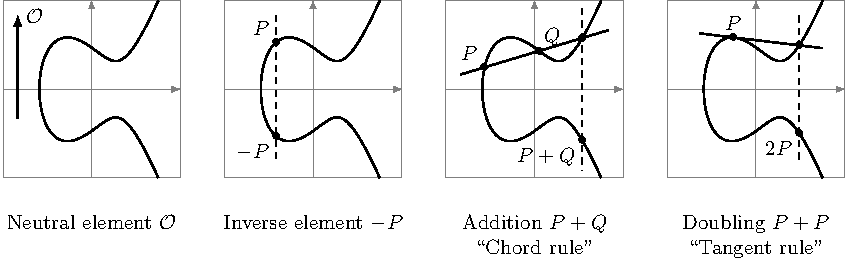
\includegraphics{ecc/ec_group_operations.pdf}
\caption{Geometric Representation of Elliptic Curve Group Operation}
 \label{fig:oper}
\end{figure}

All the points on an elliptic curve form an abelian group. We assume that every vertical line passes through a point called neutral element or point of infinity $ \cal O$ as shown in the \figref{fig:oper}. Inverse element of a point P, $P^{-1}$ is the point of intersection of the vertical line through P and the curve as seen in \figref{fig:oper}. The group operation for Elliptical Curve is called Point Addition and denoted by $P+Q$, where P and Q are points on the curve. Let $\diamond$ operator on points P and Q on the curve represent the intersection point of the line joining P and Q and the curve. Then the point addition can be represented as $\cal O \diamond (P \diamond Q)$. In other words, it represents the intersection of the vertical line through $P \diamond Q$ and the curve depicted in \figref{fig:oper}. The doubling of P, i.e P+P, is represented by similarly by taking the intersection of the tangent at P and the curve and drawing a vertical line through that point to get its intersection with the curve as shown in figure \figref{fig:oper}.

\paragraph{Algebraic Representation.} We can also represent the group operation algebraically for finite fields. The slope for the line between point P(x1,y1) and Q(x2,y2) is $D = \frac{y2-y1}{x2-x1} \mod p$. Thus the equation for the line will be  $y = D(x-x1) + y1 \mod p$. To find the intersection of the line with the curve, we will substitute the value of y to get ${(D(x-x1) + y1)}^2 = x^3 + ax + b \mod p$. The solution of this equation are x1 , x2 and $x3 = D^2-x1-x2 \mod p$, which gives $y3 = D(x3-x1) + y1 \mod p$. The pseudo code to get the Point Addition between two points P and Q is discussed in Algorithm \ref{algo}. The pseudo code also handles the corner cases where the P or Q is $\cal O$, then the result will be the other point as $P+\cal O = P$. In case the points are symmetric, the point addition will return $\cal O$ as $P + P^{-1}=\cal O $. Finally in case of point doubling, the slope with be the slope of the tangent at that point.

\makeatletter
\def\BState{\State\hskip-\ALG@thistlm}
\makeatother

\begin{algorithm}
\caption{PointAddition Algorithm with input P(x1,y1) and Q(x2,y2) }\label{algo}
\begin{algorithmic}[1]
\Procedure{PointAddition}{}
\If {$P = \cal O$}
return Q
\EndIf
\If {$Q = \cal O$}
return P
\EndIf
\If {$x1 = x2$ and $y1 = -y2$}
return $\cal O$
\EndIf
\If{$x1 = x2$ and $y1 = y2$}
\State $D \gets \frac{3*{x1}^2+a}{2*y1} \mod p$
\Else 
\State $D \gets \frac{y2-y1}{x2-x1} \mod p$
\EndIf
\State $x3 \gets D^2-x1-x2 \mod p$
\State $y3 \gets D(x3-x1) + y1 \mod p$
\State return (x3,-y3)
\EndProcedure
\end{algorithmic}
\end{algorithm}

Interestingly, the point addition is an abelian group operation as it satisfies all four properties for group operation plus commutative property.
\begin{itemize}
\item Closure Property. P+Q lies on the curve for all P and Q, as discussed earlier.
\item Associative Property. (P+Q)+R = P+(Q+R)
\item Inverse Property. $P + P^{-1} = \cal O $ where $P^{-1} = (-x,y)$ for P=(x,y). Also ${\cal O}^{-1} = \cal O$. Since line passing through P and $P^{-1}$ is a vertical line, it passes through $\cal O$.
\item Identity Property. P+$\cal O$ = P, as the vertical line intersects the inverse point $P^{-1}$, and vertical line through $P^{-1}$ intersect $P$. Thus the point of infinity is an identity for the group.
\item Commutative Property. P+Q = Q +P, as the line passing through P and Q, will be the same in both cases.
\end{itemize}

\paragraph{Scalar Multiplication.} Scalar multiplication $nP$ is equivalent to adding P to itself n times. This is analogous to exponentiation in $Z_p$ and can be computed by point double and add algorithm similar to square and multiply in case of integers. We can also pick generator P that defines a cyclic subgroup of E such that $0P, 1P, 2P, 3P \dots qP$ all lies on the curve. 

\paragraph{Building Elliptic Curve Groups.} Earlier people used to find suitable curves by a deterministic algorithm that picks a large prime p and random a and b to define a curve. Then we can determine the size of the group in polynomial time using Schoof algorithm. The size of the group should be large and prime for security reasons. Finally, pick a point P on the curve to be a generator. This process was very slow. Recently, these curves and generator point P have been standardized instead. Some examples of such curves are NIST curves, Curve25519. 







\newpage
\input{notation}
%\newpage
%\input{ciphers}
\newpage
\input{ciphers-draft}
\newpage
\section{PRF and PRP Security}
\label{sec:prf}

A standard goal for cipher security is security in the sense of pseudorandom permutations and/or pseudorandom functions. For simplicity, we will focus on \textbf{block ciphers}, which for keyspace $\keyspace=\bits^k$ and message space $\msgspace=\bits^n$ are defined by $\cipherE : \bits^k \times \{0,1\}^n \to \bits^n$. Let $\Perm(n)$ be the set of all permutations on $n$ bits. Notice that since $|\bits^n| = 2^n$, then $|\Perm(n)| = 2^n!$. Let $\Func(n,n)$ be the set of all functions from $\bits^n \to \bits^n$. Note that $|\Func(n,n)| = (2^n)^{2^n}$.

\subsection{PRF security}

We now define a \textbf{pseudorandom function} (PRF) as a function that is indistinguishable from a random function (RF). At a high level this means that the input-output behavior of some block cipher $\cipherE_K$ ``looks like'' the input-output behavior of a random function assuming key $K$ is kept secret. There are two games defined for PRF security: PRF1 and PRF0. The pseudocode for both is provided in \figref{fig:prf}. In PRF1, the adversary has access to an $\Fn$ oracle that returns the output from the block cipher $\cipherE_K$. However, in PRF0 the adversary instead receives the output from a random function $\rho$ when it queries the $\Fn$ oracle. The adversary $\advA$ does not know in which game it is playing and must query the $\Fn$ oracle to distinguish between $\cipherE_K$ and $\rho$. Adversary $\advA$ returns a bit signifying which game it believes it is in. The PRF advantage for $\advA$ is defined as 
\begin{equation*}
\AdvPRF{\cipher}{\advA} = \left| \Prob{\PRF1_\cipher^\advA\Rightarrow 1} 
- \Prob{\PRF0_\cipher^\advA\Rightarrow1} \right|.
\end{equation*}

The adversary $\advA$ wins if the probability that $\advA$ outputs 1 in game $\PRF1_\cipher^\advA$ is far greater than the probability that it outputs 1 in game $\PRF0_\cipher^\advA$. In particular, notice that if $\advA$ simply always output 1, $\AdvPRF{\cipher}{\advA}$ would be 0 as expected, since $\advA$ did not successfully distinguish $\cipher$ from a random function. 

\begin{figure}[H]
	\centering
	\hfpages{.15}{
		\underline{$\PRF1_{\cipher}^\advA$}\\
		$K \getsr \keyspace$\\
		$b' \getsr \advA^\Fn$\\
		Return $b'$\medskip
		
		\underline{$\Fn(M)$}\\
		Return $\cipherE_K(M)$
	}{
		\underline{$\PRF0_{\cipher}^\advA$}\\
		$\rho \getsr \Func(n,n)$\\
		$b' \getsr \advA^\Fn$\\
		Return $b'$\medskip
		
		\underline{$\Fn(M)$}\\
		Return $\rho(M)$
	}	
\caption{The PRF security games.}
\label{fig:prf}
\end{figure} 

Just as we provided a generic attack for TKR security using the exhaustive key search attack, is there a generic distinguishing attack for any cipher? One interesting observation is that for a given key, a block cipher $\cipherE_K$ is a permutation, meaning that two different inputs cannot produce the same output. (If this were not the case, decryption would be impossible.) However, a random function simply chooses outputs at random, so it is entirely possible for two different inputs to produce the same output. The probability of choosing $q$ values at random from $\{0,1\}^n$ and for two of these values to be the same is approximately $\frac{q^2}{2^n}$. This is colloquially known as the \textbf{birthday paradox}, since it implies that the number of people expected to produce two individuals with the same birthday is far fewer than what one might expect. The following is a more exact approximation of this birthday bound. 

\begin{theorem}(Birthday bound)
	\label{thm:bday}
	Let $C(N,q)$ be the probability that when we choose $q\geq 1$ values uniformly at random from set $\{1,2,\ldots,N\}$, with $N \geq q$, not all values chosen are distinct. Then
	\begin{align*}
		C(N,q) &\leq \frac{q(q-1)}{2N} \\
		C(N,q) &\geq 1 - e^{-q(q-1)}/2N.
	\end{align*}
	If $1 \leq q \leq \sqrt{2N}$ then
	\begin{equation*}
		C(N,q) \geq 0.3 \cdot \frac{q(q-1)}{N}.
	\end{equation*}
\end{theorem}

The interested reader may refer to \cite{BellareRogawayBook} for the proof of \thref{thm:bday}.
 
With this observation in mind, notice that if an adversary $\advA$ playing the PRF game were to query its $\Fn$ oracle enough times, eventually the probability that a repeat value is produced would be large enough and $\advA$ could then check to see if such a repeat value exists. If no repeat occurs, then $\advA$ can assume it is in game $\PRF1_{\cipher}$; otherwise, $\advA$ must be in game $\PRF0_{\cipher}$. This attack is called the \textbf{birthday attack}. We present this more formally with the following.

\begin{clm}
	\label{clm:bday}
	Let $\cipherE\Colon\bits^k \times \{0,1\}^n \to \bits^n$ be a block cipher. For $2 \leq q \leq 2^{(n+1)/2}$, there is an adversary $\advA_\text{bday}$ making $q$ $\Fn$ queries and having running time of $\calO(q)$, such that
	\begin{equation*}
		\AdvPRF{\cipher}{\advA_\text{bday}} \geq 0.3 \cdot \frac{q(q-1)}{2^n}.
	\end{equation*}
\end{clm} 

\begin{proof}
	We show the pseudocode for $\advA_{\text{bday}}$ below. 
	
	\begin{center}
		\fpage{.35}{
			\underline{\textbf{adversary} $\advA^\Fn_{\text{bday}}$} \\
			Let $M_1, M_2, \cdots, M_q \getsr \{0,1\}^n$ be distinct \\
			For $i=1, \cdots, q$ do $C_i \gets \Fn(M_i)$ \\
			If $C_1, \cdots, C_q$ are all distinct then return 1 \\
			Else return 0	
		}
	\end{center}
	
	In addition to creating $q$ messages and querying $\Fn$ $q$ times, $\advA_{\text{bday}}$ must check to see if there are any duplicates in its answered queries. Overall, $\advA_{\text{bday}}$ will then have running time of $\calO(q)$.
	To bound the advantage of $\advA_{\text{bday}}$, first notice that in game $\PRF1_{\cipher}$, $\Fn$ outputs the value from $\cipher$, so all output values will be distinct. Thus, $\advA_{\text{bday}}$ will always return 1 and $\Prob{\PRF1_\cipher\Rightarrow 1}=1$. 
	
	The probability that $\advA_{\text{bday}}$ returns 1 in game $\PRF0_{\cipher}$ is trickier to bound. In game $\PRF0_{\cipher}$, $\Fn$ returns the output from a random function and since $M_1, \cdots, M_q$ are all distinct, then $C_1, \cdots, C_q$ are independently distributed, random values from $\bits^n$. The probability that all these values are distinct is the probability that there does not exist a collision, which is $1-C(N,q)$, where $N=2^n$. 
	The PRF-advantage of $\advA^\Fn_{\text{bday}}$ is then defined as 
	\begin{align*}
	\AdvPRF{\cipher}{\advA_\text{bday}} &= \left| \Prob{\PRF1_\cipher^{\advA_\text{bday}}\Rightarrow 1} 
	- \Prob{\PRF0_\cipher^{\advA_\text{bday}}\Rightarrow1} \right| \\
	&= 1 - (1 - C(2^n,q)) \\ 
	&= C(2^n,q) \\ 
	&\geq 0.3 \cdot \frac{q(q-1)}{2^n}.
	\end{align*}
\end{proof} 

In order for $\advA_{\text{bday}}$ to have a high probability of succeeding, we expect $q \approx 2^{n/2}$. This means $\advA_{\text{bday}}$ will also have running time of about $2^{n/2}$. For large values of $n$, this becomes an impractical attack. 


\subsection{PRP security} 
We define a \textbf{pseudorandom permutation} (PRP) as a function that is indistinguishable from a random permutation (RP). The games for PRP security are provided in \figref{fig:prp}. These games work similarly to the PRF games but now utilize a random permutation in $\PRP0_\cipher^\advA$ rather than a random function. The PRP advantage for $\advA$ is defined as 
\begin{equation*}
\AdvPRP{\cipher}{\advA} = \left| \Prob{\PRP1_\cipher^\advA\Rightarrow 1} 
- \Prob{\PRP0_\cipher^\advA\Rightarrow1} \right|.
\end{equation*}

\begin{figure}
	\centering
	\hfpages{.15}{
		\underline{$\PRP1_{\cipher}^\advA$}\\
		$K \getsr \keyspace$\\
		$b' \getsr \advA^\Fn$\\
		Return $b'$\medskip
		
		\underline{$\Fn(M)$}\\
		Return $\cipherE_K(M)$
	}{
		\underline{$\PRP0_{\cipher}^\advA$}\\
		$\pi \getsr \Perm(n)$\\
		$b' \getsr \advA^\Fn$\\
		Return $b'$\medskip
		
		\underline{$\Fn(M)$}\\
		Return $\pi(M)$
	}
\caption{The PRP security games.}
\label{fig:prp}	
\end{figure}

Considering that these notions are similar, can we relate them to each other? Intuitively, there is no difference between a random function and a random permutation when observing only a few input-output pairs, as long as the ciphertext space $n$ is sufficiently large. We formalize this intuition with the following lemma. 

\begin{lem}[PRF-PRP Switching Lemma]
	\label{switching-lem}
	Let $\cipher$ be a cipher with ciphertext space $\bits^n$. 
	Let $\advA$ be an adversary making at most $q$ queries. Then
	\bnm
	\left| \Prob{\PRF0_\cipher^\advA\Rightarrow 1} 
	- \Prob{\PRP0_\cipher^\advA\Rightarrow1} \right| \le \frac{q^2}{2^n}  \;.
	\enm
\end{lem}

The intuition for the following proof is that if you have oracle access to a random function or a random permutation, then you need to make enough queries to witness a collision, as determined by the birthday bound. 

One's first instinct might be to bound the difference using a conditioning argument. For instance, let $\mathsf{Dist}$ be the event that in game $\PRF0_{\cipher}^\advA$ all values returned from oracle $\Fn$ are distinct. Then one might say that $\Prob{\PRP1_\cipher^\advA\Rightarrow 1} =   \Prob{\PRP0_\cipher^\advA\Rightarrow1 | \mathsf{Dist}}$. However, this is incorrect and in fact $\Prob{\PRP1_\cipher^\advA\Rightarrow 1} \neq   \Prob{\PRP0_\cipher^\advA\Rightarrow1 | \mathsf{Dist}}$. Refer to \cite{bellare2006multi} for further technical details. 

To correctly prove this, we will instead use a game-playing argument. We first provide the following definitions and lemma. 

\begin{definition}
	A \textbf{flag} is a variable in a pseudocode game that is set upon the occurrence of some event in the game. 
\end{definition}

Typically, games will utilize a flag called \textit{bad} which is set to $\true$.  

\begin{definition}
	Games $\G1$ and $\G2$ are \textbf{identical-until-bad} if they both contain a flag $\bad$  and their code differs only in statements following the setting of $\bad$ to $\true$. 
\end{definition} 

\begin{lem}[Fundamental Lemma of game playing \cite{bellare2006security}]
	Let $\G$, $\Hgame$ be games that are identical-until-bad and let $y$ be any
	value. Then
	\bnm
	\big| \Prob{\G\Rightarrow y} 
	- \Prob{\Hgame\Rightarrow y} \big| \le \Prob{\Hgame\setsbad} = \Prob{\G\setsbad}  \;.
	\enm
\end{lem}

Stated another way, this lemma tells us about the advantage an adversary gains in distinguishing a pair of identical-until-bad games, $\G$ and $\Hgame$. Since $\G$ and $\Hgame$ only differ upon the setting of flag $\bad$, then intuitively we can see that the advantage of an adversary to distinguish between these games must be at most the probability that $\bad$ is set during its execution.

The overall technique we will implement here (and generally in game-playing arguments) is to create a chain of games that are identical-until-bad. We can then invoke the Fundamental Lemma of game playing to upper-bound the adversary's advantage by the probability that $\bad$ gets set in either game. We can slowly modify the games in ways that change the probability of $\bad$ being set until we reach some terminal game where we can utilize conventional probabilistic methods to bound the probability of setting $\bad$. Note that the following proof introduces a $\bad$ flag that can be immediately bounded by traditional means without modification, although future proofs we will see will require further transformations. 

\begin{proof}[Proof of \lemref{switching-lem}]
	 We define the games in \figref{fig:switching}. Notice that the output from game $\G0$ has an identical distribution to that of game $\PRP0_\cipher^\advA$. The only difference between them is that game $\PRP0_\cipher^\advA$ chooses a random permutation and returns the output from that, while game $\G0$ chooses unique values at random as $\advA$ makes queries to $\Fn$. Then $\Prob{\PRP0_\cipher^\advA\Rightarrow1} = \Prob{\G0}$. Game $\G1$ includes the boxed statement and also has an identical output distribution to that of game $\G0$. It simply chooses an output value at random, and if it detects a repeat it then chooses another unique value. In the case of a repeat, it also sets the $\bad$ flag to $\true$. We then have that $\Prob{\G1} = \Prob{\G0}$. We next transition to game $\G2$ and notice that $\G1$ and $\G2$ are \textbf{identical-until-bad}. The Fundamental Lemma of game playing then states that $\Prob{\G1} \leq \Prob{\G2} + \Prob{\bad \text{ set to } \true}$. Game $\G2$ returns values chosen at random and allows for repeat values, so it has an identical output distribution to $\PRF0_\cipher^\advA$. This means $\Prob{\PRF0_\cipher^\advA\Rightarrow1} = \Prob{\G2}$. Finally, the probability that $\bad$ is set to $\true$ is the probability that a random value is chosen by $\Fn$ such that it is not distinct, which is bounded by the birthday bound. We then have the following:
	 
	 \begin{figure}
	 	\centering
	 	\hfpagess{.20}{.20}{
	 		\underline{$\G0$}\\[2pt]
	 		$b' \getsr \advA^\Fn$\\
	 		Return $b'$\medskip
	 		
	 		\underline{$\Fn(M)$}\\
	 		If $\TabF[M] = \bot$ then\\
	 		\ind $\TabF[M] \getsr \bits^n \setminus \TabF$\\
	 		Return $\TabF[M]$
	 	}{
	 		\underline{\fbox{$\G1$} \;\;\; $\G2$}\\[2pt]
	 		$b' \getsr \advA^\Fn$\\
	 		Return $b'$\medskip
	 		
	 		\underline{$\Fn(M)$}\\
	 		$C \getsr \bits^n$\\
	 		If $C \in \TabF$ then\\
	 		\ind $\badtrue$\\
	 		\ind \fbox{$C \getsr \bits^n \setminus \TabF$}\\
	 		$\TabF[M] \gets C$\\
	 		Return $\TabF[M]$
	 	}
	 	\caption{The games for the proof of the PRF-PRP Switching Lemma (\lemref{switching-lem}).}
	 	\label{fig:switching}	
	 \end{figure} 
	 
	 \begin{align*}
	 \left| \Prob{\PRP0_\cipher^\advA\Rightarrow 1} 
	 - \Prob{\PRF0_\cipher^\advA\Rightarrow1} \right|  
	 &=  \left|\Prob{\G0} - \Prob{\PRF0_\cipher^\advA\Rightarrow1} \right|  \\
	 &=  \left|\Prob{\G1} - \Prob{\PRF0_\cipher^\advA\Rightarrow1} \right|  \\
	 &\le \left|\Prob{\G2} + \Prob{\bad \text{ set to } \true} - \Prob{\PRF0_\cipher^\advA\Rightarrow1} \right|\\
	 &= \Prob{\bad \text{ set to } \true}\\
	 &\le \frac{q^2}{2^n} \\
	 \end{align*} 
\end{proof}
\input{prp/all}
\newpage
\input{cryptanalysis}
\newpage
\input{freqanalysis}
\newpage
\input{tweakciphers}
\newpage
\input{symenc}
\newpage
\input{authenc}
\newpage
\input{msgauth}
\newpage
\input{genericcomp}
\newpage
\input{advanced-ae}
\newpage
\input{aepractice}
\newpage
%%%%%%%%%%%%%%%%%%%%%%%%%%%%%%%%%%%%%%%%%%%%%%%%%%%%%%%%%%%%%%%%%%%%%%%%%%%%%%%%
\section{Cryptographic Hash Functions}
\label{sec:hashfunctions}

\begin{wrapfigure}{r}{2in}
  \centering
    \begin{tikzpicture}[scale=0.4]
        \node[draw,trapezium,trapezium left angle=70,trapezium right angle=70,minimum height=1.0cm,thick,shift={(1.15,0)},rotate=-90] (hfxn)
        {\begin{sideways}\Large $\hash$ \end{sideways}};
        \draw[->,thick] (0,0) node[left] {$M$} -- (hfxn);
        \draw[->,thick] (hfxn) -- ++(3,0) node[right] {$H(M)$};
    \end{tikzpicture}
    \caption{An abstract hash function, where $M$ is the message and $H(M)$ the corresponding hash (or ``digest'')}
\label{fig:hash-function}
\end{wrapfigure}

A \emph{cryptographic hash function (CHF)} is a map $H\Colon\msgspace\rightarrow\bits^n$, i.e. deterministic function, for
some set $\msgspace$ and number $n > 0$. 
CHFs are a highly useful building blocks for secure applications, because the allow to derive a concise integer representation, that is hard to forge, from an arbitrary large input message.
Typical values of $n$ these days are 256, 512, or 1024, and most hash functions support an essentially unlimited message space $\msgspace$, such as all strings of length up to $2^{64}-1$.

CHFs enable us to prove the integrity or existence of a binary blob without having to transfer the entire data, which allows to increase efficiency in many use cases. They further are hard to inverse, i.e. it is non-trivial to derive the input value (or \emph{message}) from the hash value (or \emph{digest}).
Applications of CHFs include, but are not limited to, file comparison, digital signatures, message authenticated codes, key derivation, password hashing.

\subsection{Collision Resistance}
Collision resistance is one of the most important security properties of hash functions.
This property guarantees that it is very hard for an adversary to find two messages that correspond to the same hash, which ensures that the same cryptographic signature cannot be reused by an attacker for a different message.

\begin{wrapfigure}{r}{2in}
\fpage{.3}{
    \underline{$\advA_{Cr}$}\\[1pt]
For i = 1 to q do: \\
\myInd $X_i \getsr {\{0, 1\}}^m$\\
\myInd $h_i \leftarrow H(X_i)$\\
If $\exists i,j$ s.t. $X_i \neq X_j \land h_i \neq h_j$ then\\
\myInd Return $(X_i, X_j)$\\
Return \false
}
\end{wrapfigure}


On a high level, the \emph{pigeonhole principle} states that functions that map from a large space there exists an efficient adversary that is able to find a collision.
However, Rogaway showed that these are non-trivial to find for a human adversary~\cite{rogaway2006formalizing}.
Thus, the birthday attack is most efficient known attack against cryptographic hash functions and will be described in the following.

\begin{theorem*}
For a regular hash function, probability that an attacker $A_{Cr}$ finds a collision is $\ge 0.3 \frac{q(q-1)}{2^n}$, where $q$ is the number of messages queried by $A_{Cr}$.
\end{theorem*}

\begin{proof}
    $A_{Cr}$ picks $q$ messages independently at random. We can then derive the probability that a collision is found after $A_{Cr}$ ran as the following. Here ${Coll}_i$ represents the probability that a chosen value $Y_i$ is equal to a previous value $Y_j$.

\begin{align*}
    Pr[Coll] = Pr[{Coll}_1 \lor {Coll}_2 \lor \dots \lor {Coll}_q] \\
             \geq Pr[{Coll}_1] + Pr[{Coll}_2] + \dots + Pr[{Coll}_q] \\
             = \frac{0}{2^n} + \frac{1}{2^n} + \dots + \frac{q}{2^n} \\
             = \frac{q(q-1)}{2^n}
\end{align*}

For a regular hash function this bound is even tighter.
We define regular in this context as the property that each point in the range of the function maps to the same number of input points.
In other words, each point in the range has the same number of pre-images (see Section \ref{sec:hashfunctions2} for a discussion on pre-images and pre-image resistance).
In this case the bound is equal to the regular birthday probability~\scribenote{Do we need a proof for that? I was not able to find one}.

$$
    Pr[Coll] \geq 0.3 \frac{q(q-1)}{2^n}
$$
\end{proof}

\subsection{Building a Cryptographic Hash Function}
\begin{wrapfigure}{r}{2in}
    \centering
\fpage{.25}{
    \underline{$\advA(K)$}\\[1pt]
$M \leftarrow E_k(0^n) \xor E_k(1^n) $ \\
Return $(0^n 0^n, 1^n || M)$
}
    \caption{An efficient attacker for a CBC-MAC-based hash function.}
    \label{fig:cbc-hash-attack}
\end{wrapfigure}

Now that we discussed some of the guarantees of CHFs, we will investigate how to build such a primitive.
Ideally, we would like to leverage building blocks that were introduced in previous parts of these notes.
CBC-MAC, like CHFs, takes a variable size input and converts it into a fixed size value.
In the following we discuss why CBC-MAC is \emph{not} a good hash function.


To show that CBC-MAC is unfit to be used as CHF, we sketch an efficient attack to find a hash collision.
    Our attacker $A$ (outlined in Figure \ref{fig:cbc-hash-attack}) leverages the fact that ever step of CBC-MAC uses the same encryption key, which is must be public in order to use CBC-MAC as a hash function.
$A$ then aims to compute to input values that are each two blocks wide and map to the same hash.
Here, CBC-MAC will invoke the underlying encryption function twice.
Because the encryption key is identical in both cases, all we have to ensure is that the value passed to the second encryption pass is identical as well in both cases.

To generate an identical input value, we have cancel out the output of the first encryption pass.
$A$ achieves this by first computing the desired output with the expected output. 
Setting the XOR of the two as the second part of the message will cancel out the expected, and undesired, output of the previous function.
Here, the input for the second encryption pass is $E_k(0^n) \xor E_k(1^n) \xor E_k(1^n) = E_k(0^n)$. $\qed$

\begin{wrapfigure}{r}{2.9in}
\begin{tikzpicture}[scale=0.4]
	\begin{scope}[]
		\node [draw,trapezium,trapezium left angle=50,trapezium right angle=90,minimum height=0.75cm,thick,shift={(1.15,0.3)},rotate=-90]
		{\begin{sideways}\Large$f$\end{sideways}};
		\draw[->,thick] ++(0.5,+4) node[above] {$\msg_1$} -- ++(0,-1.5) -- ++(1.4,0);
		\draw[->,thick] ++(0,0.5) node[left] {$\IV$} -- ++(1.9,0);
	\end{scope}

	\begin{scope}[shift={(3.8,0)}]
		\node [draw,trapezium,trapezium left angle=50,trapezium right angle=90,minimum height=0.75cm,thick,shift={(1.35,0.3)},rotate=-90] (centerbox)
		{\begin{sideways}\Large$f$\end{sideways}};
		\draw[->,thick] ++(0.9,+4) node[above] {$\msg_2$} -- ++(0,-1.5) -- ++(1.4,0);
		\draw[->,thick] ++(0,0.5) -- ++(2.4,0);
	\end{scope}

	\begin{scope}[shift={(8.2,0)}]
v		\node [draw,trapezium,trapezium left angle=50,trapezium right angle=90,minimum height=0.75cm,thick,shift={(1.35,0.3)},rotate=-90]
		{\begin{sideways}\Large$f$\end{sideways}};
		\draw[->,thick] ++(0.9,+4) node[above] {$\qquad\msg_3 \concat 10^r \concat \bm{\langle} \left| \msg \right| \bm{\rangle}$} -- ++(0,-1.5) -- ++(1.4,0);
		\draw[->,thick] ++(0,0.5) -- ++(2.4,0);
        \draw[->,thick] ++(4.4,0.5) -- ++(2,0) node[right] {$H(M)$};
	\end{scope}
\end{tikzpicture}
\caption{A sketch of the Merkle-Damgard Construction}
\label{fig:md-construction}
\end{wrapfigure}

\paragraph{}
We now introduce the \emph{Merkle-Damgard Construction}, which uses a similar scheme except that it changes the encryption key in every step.
The MD constructions changes the key on every step by inputting the respective part of the message as the encryption key, while the input and output of the encryption function are used to maintain state of the hashing process.
Figure \ref{fig:md-construction} outlines this scheme in more detail.

While this design seems promising it still prone to prefix attacks similar to the one outline before, when using a plain block cipher as compression function.
This mean, in order to make the MD construction safe, we need to find a better compression function.
Compression functions are a one-way function like hash functions. However, unlike hash functions, they take a constant-size block as well as a constant-size state as input, both of which must be hard to derive from the output alone.

The \emph{Davies-Meyers compression function}~\cite{winternitz1984secure,black2002black} is constructed by modifying wrapping a block cypher.
It adds a XOR operation of the encryption output with the input state before the encryption.
This makes it hard to regenerate $E_K$'s input even when knowing $K$ if $E_K$ is an \emph{ideal block cipher}.

\begin{wrapfigure}{r}{2.9in}
\begin{tikzpicture}[scale=0.4]
    \node (M) {M};
    \node [right=0.5cm of M] (M2) {};
    \node [below=1cm of M2.center] (M3) {};
    \node [right=0.5cm of M2, draw,rectangle, minimum width=1.5cm, minimum height=0.75cm,thick] (E) {$E_K$};
    \node [right=0.5cm of E, draw, circle, inner sep=-1, outer sep=0] (xor) {$\xor$};
    \node [below=1cm of xor.center] (xor2) {};
    \node [right=0.5cm of xor] (Y) {};
    \draw[thick] (M) -- (M2.center);
    \draw[->, thick] (M2.center) -- (E);
    \draw[thick] (M2.center) -- (M3.center);
    \draw[thick] (M3.center) -- (xor2.center);
    \draw[thick] (E) -- (xor);
    \draw[thick] (xor2.center) -- (xor);
    \draw[->, thick] (xor) -- (Y);
\end{tikzpicture}

\caption{The Davies-Meyers compression function}
\end{wrapfigure}

\begin{wrapfigure}{l}{3in}
\fpage{.25}{
\underline{$\CR^\advA_{H}$}\\[1pt]
$(M,M') \getsr \advA$\\
If $M = M'$ then Ret $\false$\\
Ret $H(M) = H(M')$
}

\bnm
\AdvCR{H}{\advA} = \Prob{\CR^\advA_H\Rightarrow\true}
\enm

\fpage{.25}{
\underline{$\CR^\advA_{H,\ic}$}\\[1pt]
$(E, D) \getsr \blockciphers(k,n)$\\
$(M,M') \getsr \advA^{\ic,\icInv}$\\
If $M = M'$ then Ret $\false$\\
Ret $H^\ic(M) = H^\ic(M')$\medskip

\underline{$\ic(K,X)$}\\
Ret $\cipherE(K,X)$\medskip

\underline{$\icInv(K,Y)$}\\
Ret $\cipherD(K,Y)$
}
\end{wrapfigure}

\begin{theorem*}
Let $f$ be the Davies-Meyer compression function built from a block cipher
$\cipherE\Colon\bits^k\times\bits^n\rightarrow\bits^n$ modeled as an ideal
cipher and let $D$ be the associated decryption function.
For any adversary $\advA$ making at most~$q$ queries it holds that
\bnm
  \AdvCR{f}{\advA} \le \frac{(q+1)(q+2)}{2^n} \;.
\enm
\end{theorem*}

\begin{proof}
Assume $\advA$ that outputs $(Y,M)$ and $(Y',M')$ has already queried $\cipherE$
or $\cipherD$ for associated points. This can be argued easily by reducing to
by making at most $q' = q+2$ queries.
Then each query defines a triple $(K_i,X_i,Y_i)$ where either $Y_i = \cipherE(K_i,X_i)$ was queried or $X_i =
\cipherD(K_i,Y_i)$ was queried. For a collision to occur it must be that there
exist indices $i,j$ such that $X_i \oplus Y_i = X_j \oplus Y_j$, to arrange that
$X_i \oplus \cipherE(K_i,X_i) = X_j \oplus \cipherE(K_j,X_j)$. Let $C_j$ be the
event that such a collision occurs upon a query the $j\thh$ query. Then we have
that $X_i,Y_i$ are at this point fixed values while exactly one of $X_j$ or
$Y_j$ is a fixed value, with the other being a uniformly chosen point subject
only to permutivity. Then we have that 
\begin{align*}
\Prob{\CR_{f,\cipherE}^\advA\Rightarrow\true} 
    &\le \sum_{j=1}^{q'} \Prob{C_j}  &  \\
    &\le \sum_{j=1}^{q'} \frac{j-1}{2^n-j+1} &\\
    &\le \sum_{j=1}^{q'} \frac{j-1}{2^n-q'} &\\
    &= \frac{q'(q'-1)}{2(2^n-q')} & \\
    &\le \frac{(q+2)(q+1)}{2^n} &( \text{assuming }q' \leq 2^{n-1} ) \\
\end{align*}
\end{proof}

\subsection{Attacks on MD5 and SHA-1}



\begin{theorem*}
Let $f$ be a compression function and $H$ be the MD hash function built from it. 
Let $\advA$ be a $\CR_H$-adversary outputing messages eacah of length at most $\sigma$
blocks after MD padding. Then we give an $\CR_f$-adversary $\advB$
such that
\bnm
  \AdvCR{\advA}{H} \le \AdvCR{\advB}{f} \;.
\enm
Adversary~$\advB$ runs in time that of $\advA$ plus at most $2\sigma$ computations of
$f$.
\end{theorem*}


\fpage{.25}{
\underline{$\CR^\advA_{H,\ic}$}\\[1pt]
$E \getsr \blockciphers(k,n)$\\
$(M,M') \getsr \advA^{\ic,\icInv}$\\
If $M = M'$ then Ret $\false$\\
Ret $H^\ic(M) = H^\ic(M')$\medskip

\underline{$\ic(K,X)$}\\
If $\TabE[K,X] \ne \bot$ then\\
\myInd $Y \getsr \Range[K]$\\
\myInd $\TabE[K,X] \getsr Y$\\
\myInd $\TabD[K,Y] \getsr X$\\
\myInd $\Domain[K] \getu X$\\
\myInd $\Range[K] \getu Y$\\
Ret $\TabE[K,X]$\medskip

\underline{$\icInv(K,Y)$}\\
If $\TabD[K,Y] \ne \bot$ then\\
\myInd $X \getsr \Domain[K]$\\
\myInd $\TabE[K,X] \gets Y$\\
\myInd $\TabD[K,Y] \gets X$\\
\myInd $\Domain[K] \getu X$\\
\myInd $\Range[K] \getu Y$\\
Ret $\TabD[K,Y]$
}



\newpage
%%%%%%%%%%%%%%%%%%%%%%%%%%%%%%%%%%%%%%%%%%%%%%%%%%%%%%%%%%%%%%%%%%%%%%%%%%%%%%%%
\section{Further Security Properties for Hash Functions}
\label{sec:hashfunctions2}

\fpage{.25}{
\underline{$\OWF^\advA_{H}$}\\[1pt]
$M \getsr \msgspace$\\
$Y \gets H(M)$\\
$M' \getsr \advA(Y)$\\
Ret $(H(M') = Y)$
}


\bnm
\AdvOWF{H}{\advA} = \Prob{\OWF^\advA_H\Rightarrow\true}
\enm



\fpage{.25}{
\underline{$\SPR^\advA_{H}$}\\[1pt]
$M \getsr \msgspace$\\
$Y \gets H(M)$\\
$M' \getsr \advA(M)$\\
Ret $(H(M') = H(M)) \land (M \ne M')$
}


\bnm
\AdvSPR{H}{\advA} = \Prob{\SPR^\advA_H\Rightarrow\true}
\enm


\fpage{.25}{
\underline{$\PWR^\advA_{H,p}$}\\[2pt]
$\pw \get{p} \msgspace$\\
$\salt \getsr \bits^n$\\
$Y \gets H(\salt \concat M)$\\
$\pw' \getsr \advA(\salt,Y)$\\
Ret $(\pw' = \pw)$
}

\fpage{.25}{
\underline{$\PWR^\advA_{\Horacle,p}$}\\[2pt]
$\pw \get{p} \msgspace$\\
$\salt \getsr \bits^n$\\
$Y \gets \Horacle(\salt \concat M)$\\
$\pw' \getsr \advA^\Horacle(\salt,Y)$\\
Ret $(\pw' = \pw)$\medskip

\underline{$\Horacle(M)$}\\
If $\TabH[M] = \bot$ then\\
\myInd $\TabH[M] \getsr \bits^n$\\
Ret $\TabH[M]$
}

\begin{theorem*}
Let $H\Colon\msgspace\rightarrow\bits^n$ and $\advA$ be a $\SPR_H$-adversary.
Then we give a $\CR_H$-adversary $\advB$ such that
\bnm 
  \AdvSPR{H}{\advA} \le \AdvCR{H}{\advB}
\enm
Adversary~$\advB$ runs in time that of $\advA$. 
\end{theorem*}


\paragraph{Application: password recovery.}
The min-entropy of a distribution $p$ is the probability that one can guess a
value chosen according to $p$ in a single guess. Mathematically:

\bnm
  \Hinfty(p) = -\max_{x} \log \frac{1}{p(x)}
\enm
Not to be confused with Shannon entropy:

\bnm
  \Hshan(p) =  \sum_x p(x) \log \frac{1}{p(x)}
\enm

\begin{theorem}
Let $\Horacle\Colon\msgspace\rightarrow\bits^n$ be modeled as a random oracle
and $p$ be a distribution over $\msgspace$.
Then for any $\PWR_{\Horacle,p}$-adversary $\advA$ making at most $q$ queries 
it holds that
\bnm
  \AdvPWR{\Horacle,p}{\advA} \le \frac{q}{2^{\mu(p)}} \;.
\enm
\end{theorem}



\hfpages{.25}{
\underline{$\PRF1_{F,\Horacle}^\advA$}\\
$K \getsr \keyspace$\\
$b' \getsr \advA^{\Fn,\Horacle}$\\
Return $b'$\medskip

\underline{$\Fn(M)$}\\
Return $F^\Horacle_K(M)$\medskip

\underline{$\Horacle(X)$}\\
If $\TabH[X] = \bot$ then\\
\myInd $\TabH[X] \getsr \bits^n$\\
Ret $\TabH[X]$

}{
\underline{$\PRF0_{F,\Horacle}^\advA$}\\
$\rho \getsr \Func(\msgspace,n)$\\
$b' \getsr \advA^{\Fn,\Horacle}$\\
Return $b'$\medskip

\underline{$\Fn(M)$}\\
Return $\rho(M)$\\

\underline{$\Horacle(X)$}\\
If $\TabH[X] = \bot$ then\\
\myInd $\TabH[X] \getsr \bits^n$\\
Ret $\TabH[X]$
}


\begin{theorem}
Let  $\Horacle\Colon\msgspace\rightarrow\bits^n$ be modeled as a random oracle
and let $F^\Horacle\Colon\keyspace\times\msgspace\rightarrow\bits^n$ be the
hash-based PRF defined as $F^\Horacle(K,M) = \Horacle(K \concat M)$. 
Then for any $\PRF_{F,\Horacle}$-adversary $\advA$ making at most $q$ queries 
to $\Horacle$ it holds that
\bnm
  \AdvPRF{F,\Horacle}{\advA} \le \frac{q}{|\keyspace|} \;.
\enm
\end{theorem}



\hfpages{.25}{
\underline{$\INDIFF1_{H,\foracle}^\advD$}\\
$b' \getsr \advD^{\Fn,\foracle}$\\
Ret $b'$\medskip

\underline{$\Fn(M)$}\\
Ret $H^\foracle(M)$\medskip

\underline{$\foracle(X)$}\\
If $\Tabf[X] = \bot$ then\\
\myInd $\Tabf[X] \getsr \bits^n$\\
Ret $\Tabf[X]$
}{
\underline{$\INDIFF0_{\Horacle,\simu}^\advD$}\\
$b' \getsr \advD^{\Fn,\simoracle}$\\
Return $b'$\medskip

\underline{$\Fn(M)$}\\
If $\TabH[M] = \bot$ then\\
\myInd $\TabH[M] \getsr \bits^n$\\
Ret $\TabH[M]$\medskip

\underline{$\simoracle(X)$}\\
Ret $\simu^\Fn(X)$
}


\bnm
  \AdvINDIFF{H,\foracle,\simu}{\advA} =
    \left|\Prob{\INDIFF1_{H,\foracle}^\advD\Rightarrow1} -
            \Prob{\INDIFF0_{\Horacle,\simu}^\advD\Rightarrow1}\right|
\enm


\hfpages{.20}{
\underline{$\RKAPRF1_{F,\Phi}^\advA$}\\
$K \getsr \keyspace$\\
$b' \getsr \advA^{\Fn}$\\
Ret $b'$\medskip

\underline{$\Fn(\phi,X)$}\\
If $\phi \notin \Phi$ then\\
\myInd Ret $\bot$\\
Ret $F(\phi(K),X)$
}{
\underline{$\RKAPRF0_{F,\Phi}^\advA$}\\
$K \getsr \keyspace$\\
$\rho \getsr \Func(\keyspace\times\msgspace,n)$\\
$b' \getsr \advA^{\Fn}$\\
Ret $b'$\medskip

\underline{$\Fn(\phi,X)$}\\
If $\phi \notin \Phi$ then\\
\myInd Ret $\bot$\\
Ret $\rho(\phi(K),X)$
}



\input{hash/all}
\newpage
\section{PRFs from Hash functions}

\subsection{Other Hash based PRFs}
The Merkle Damg{\aa}rd construction from the previous section is a type of Prefix MAC (since the key is prepended to the message). Although the construction is a secure PRF in the random oracle model, we saw how it is susceptible to length extension attacks. Several alternatives have been proposed to counter these attacks. We use $\hash^f$ to represent the Merkle Damg{\aa}rd construction with $f$ as the underlying compression function.  

\paragraph{Suffix MAC:}
$\hash^f(M \Vert K)$ - The key is appended to the end instead of the beginning. Now, for a length extension attack to succeed, the adversary must find a collision for hash output of the message prefix until the key is added. To elaborate, if the adversary finds messages $M_0$ and $M_1$ such that $\hash^f(M_0) = \hash^f(M_1)$ by an offline collision attack, then it can break security for the overall construction without ever needing the key. To prove \PRF-security, therefore, we require that $\hash$ be collision resistant.


\paragraph{Envelope MAC:} $\hash^f(K_1 \Vert M \Vert K_2)$ - A key $K_1$ is prepended and another key $K_2$ is appended to the input. The \PRF-security proof is similar to the one before except now collision resistance is no longer required.

\paragraph{Nested MAC:}
$\hash^f(K_1 \Vert \hash^f(K_2 \Vert M))$ - The standard Prefix MAC construction is applied to the message twice with two \textit{independently} chosen keys $K_1$ and $K_2$.


\subsection{The HMAC Construction}

$\HMAC$, a widely used MAC in practice is a close variant of the nested MAC. For $\HMAC$, The keys $K_1$ and $K_2$ are no longer picked independently but rather derived from some base key $K$. The keys are computed as $K_1 = f(\IV, K \oplus \ipad)$ and $K_2 = f(\IV, K \oplus \opad)$ where $\ipad$ (inner pad) and $\opad$ (outer pad) are constants. The usage of a single base key rather than two allows $\HMAC$ to be built using existing SHA hash functions in a black-box way. Figure \ref{fig: HMAC construction} shows both a shortened and an extended version of the $\HMAC$ construction

\begin{figure}[h]
\centering
\subcaptionbox{%
    % 
    \label{fig:HMAC 1}
  }[0.3\linewidth] {
   \begin{tikzpicture}[scale=0.4]
            \begin{scope}[]
                \node [draw,trapezium,trapezium left angle=70,trapezium right angle=70,minimum height=0.75cm,thick,fill=orange!15,shift={(1.15,0)},rotate=-90] 
                {\begin{sideways}\Large $\hash$ \end{sideways}};
                \draw[->,thick] (0,0) node[left] {$K_1 \Vert M $} -- (1.9,0);
                \draw[->,thick] ++(4,0) -- ++(1.5,0) -- ++(0,-2.5);
            \end{scope}
            \begin{scope}[shift={(6.2,-3.25)}]
                \node [draw,trapezium,trapezium left angle=70,trapezium right angle=70,minimum height=0.75cm,thick,fill=orange!15,shift={(1.15,0)},rotate=-90] 
                {\begin{sideways}\Large $\hash$ \end{sideways}};
                \draw[->,thick] (0,0) node[left] {$K_2 \Vert h$} -- (1.9,0);
                \draw[->,thick] ++(4,0) -- ++(2,0) node[right] {$Y$};
            \end{scope}
        \end{tikzpicture}
    }
\hfill
\subcaptionbox{%
   % \label{fig:HMAC 2}
  }[0.5 \linewidth]
  { 
  \begin{tikzpicture}[scale=0.4]
            \begin{scope}[]
                \node [draw,trapezium,trapezium left angle=50,trapezium right angle=90,minimum height=0.5cm,thick,fill=orange!15,shift={(1.15,0.3)},rotate=-90] 
                {\begin{sideways}\Large$f$\end{sideways}};
                \draw[->,thick] ++(0.5,+3) node[above] {$K \oplus \ipad$} -- ++(0,-1) -- ++(1.7,0);
                \draw[->,thick] ++(0,0.5) node[left] {IV} -- ++(2.2,0);
            \end{scope}

            \begin{scope}[shift={(3.5,0)}]
                \node [draw,trapezium,trapezium left angle=50,trapezium right angle=90,minimum height=0.5cm,thick,fill=orange!15,shift={(1.15,0.3)},rotate=-90] 
                {\begin{sideways}\Large$f$\end{sideways}};
                \draw[->,thick] ++(0.5,+3) node[above] {$M_1$} -- ++(0,-1) -- ++(1.7,0);
                \draw[->,thick] ++(0,0.5) -- node[below] {$K_1$} ++(2.2,0);
            \end{scope}

            \begin{scope}[shift={(7,0)}]
                \node [draw,trapezium,trapezium left angle=50,trapezium right angle=90,minimum height=0.5cm,thick,fill=orange!15,shift={(1.15,0.3)},rotate=-90] 
                {\begin{sideways}\Large$f$\end{sideways}};
                \draw[->,thick] ++(0.5,+3) node[above] {$M_2$} -- ++(0,-1) -- ++(1.7,0);
                \draw[->,thick] ++(0,0.5) --  ++(2.2,0);
            \end{scope}
            
            \begin{scope}[shift={(7,-6)}]
                \node [draw,trapezium,trapezium left angle=50,trapezium right angle=90,minimum height=0.5cm,thick,fill=orange!15,shift={(1.15,0.3)},rotate=-90] 
                {\begin{sideways}\Large$f$\end{sideways}};
                \draw[->,thick] ++(0.5,+3) node[above] {$K \oplus \opad$} -- ++(0,-1) -- ++(1.7,0);
                \draw[->,thick] ++(0,0.5) node[left] {IV} --  ++(2.2,0);
            \end{scope}
            
            \begin{scope}[shift={(10.5,-6)}]
                \node [draw,trapezium,trapezium left angle=50,trapezium right angle=90,minimum height=0.5cm,thick,fill=orange!15,shift={(1.15,0.3)},rotate=-90] 
                {\begin{sideways}\Large$f$\end{sideways}};
                \draw[->,thick] ++(0,+6.4) -- ++(0.5, 0) -- ++(0,-4.4) -- ++(1.7,0);
                \draw[->,thick] ++(0,0.5) -- node[below] {$K_2$} ++(2.2,0);
                \draw[->,thick] ++(3.6,0.5) -- ++(2,0) node[right] {$Y$};
            \end{scope}
        \end{tikzpicture} 
    }
    \caption{HMAC construction} \label{fig: HMAC construction}
\end{figure}


\subsection{Analysis of HMAC}
To analyze the PRF security of the $\HMAC$ construction, we can first prove security under the assumption that the hash function is a random oracle $\Horacle$. Notice that now the dependence of keys $K_1$ and $K_2$ no longer matters; the proof will apply for the regular Nested MAC. We leave the formal proof to the reader as \ref{Exercise 1} 

While security in the RO model is a good sanity check, it is usually not sufficient by itself. Attacks on real world hash based constructions can take advantage of the underlying structure to break security.
This naturally begs the question: What assumptions are reasonable to show security of real world constructions? We argue that it might be reasonable to assume that the underlying compression function $f$ is a good PRF to prove security. We defer further details till the next section.

What does it mean exactly for $f$ to be a ``good'' PRF here? A strawman answer would be to make sure that $f$ is secure under the standard PRF security game. Unfortunately, the standard PRF game provides no room for an adversary to use the output under a related key to distinguish between the real and ideal worlds. Recall that for $\HMAC$, $K_1$ and $K_2$ are derived from a single key $K$. Even then, ideally an adversary should not be able to correlate the outputs of $f$ under the two keys. Intuitively, we want to ask whether $K_1$ and $K_2$ are indistinguishable from random bit strings \textit{even when} the adversary can see outputs under related keys. 
We resolve this mismatch by constructing a slightly different game $\RKAPRF$ (Figure \ref{fig:RKA}). Statements modified from the original PRF game are colored blue. Suppose $f$ takes as input a $d$ bit key and an $n$ bit message and compresses them to a single $n$ bit output. That is, $f: \bits^n \times \bits^d \to \bits^n$. The game is now parametrized by a set of functions $\Phi$ and the adversary can now query the oracle using a related key $\phi(K)$ for any $\phi \in \Phi$. The adversarial advantage for the $\RKAPRF$ game is defined in the standard way:
\[
\AdvRKAPRF{f, \Phi}{\advA} = 
\left| 
    \Pr[\LRKAPRFIdeal^\advA_{f,\Phi} \Rightarrow 1] 
    - \Pr[\LRKAPRFReal^\advA_{f,\Phi} \Rightarrow 1]
\right|
\]


\begin{figure}[h]
\centering
\hfpagess{.15}{.25}{
    \underline{$\LRKAPRFIdeal^\advA_{f, \modify{\Phi}}$}\\[1pt]
    $K \getsr \bits^d$\\
    $b' \getsr \advA^{\FnOracle}$\\
    Ret $b'$\medskip

    \underline{$\FnOracle(\modify{\phi}, X)$}\\
    \modify{If $\phi \in \Phi$ then}\\
    \modify{\myInd Ret $\bot$}\\
    Ret $f(X,\modify{\phi(K)})$\medskip
}
{
    \underline{$\LRKAPRFReal^\advA_{f, \modify{\Phi}}$}\\[1pt]
    $K \getsr \bits^d$\\
    $\rho \getsr \Func(\modify{\bits^n \times \bits^d},n)$\\
    $b' \getsr \advA^{\FnOracle}$\\
    Ret $b'$\medskip

    \underline{$\FnOracle(\modify{\phi}, X)$}\\
    \modify{If $\phi \in \Phi$ then}\\
    \modify{\myInd Ret $\bot$}\\
    Ret $\rho(X \modify{, \phi(K)})$\medskip
}
\caption{Related Key Attack Game} \label{fig:RKA}
\end{figure}



We note that this game modification is far more general than what might be needed for HMAC security. For our application, it is reasonable to restrict $\Phi$ to just $\phi_{\ipad}$ and $\phi_{\opad}$ where $\phi_{\ipad}(K) = K \oplus \ipad$ and $\phi_{\opad}(K) = K \oplus \opad$ and then ask whether $f$ is \RKAPRF secure. Choosing such an $f$ function would imply that $K_1$ and $K_2$ are indistinguishable from random bit strings. 

Suppose now that we have ensured that the compression function $f$ used in HMAC is \RKAPRF secure. We still need to show that the overall construction is \PRF-secure. 

\begin{lemma}
(Informal) If $f$ is $\RKAPRF$-secure and the iterated keyed hash function $\hash$ is collision resistant then the $\HMAC$ construction is $\PRF$-secure
\end{lemma}
\begin{proofsketch}
If $f$ is $\RKAPRF$-secure, then the keys $K_1$ and $K_2$ are indistinguishable from random bit strings even for adversaries that use outputs from related key functions $\phi_{\ipad}$ and $\phi_{\opad}$. Now, we have seen that the composition of a collision resistant function and a secure PRF is a secure PRF. Therefore, we can conclude that $\HMAC$ is PRF-secure
\end{proofsketch}

\noindent Some subtleties like block padding have been ignored in the above sketch. A detailed proof can be found in \cite{Bellare1996}. A stronger result that does not rely on the collision resistance of $\hash$ (but instead on some weaker assumptions) is proved in \cite{Bellare2006}

\subsection{The Indifferentiability Framework}
We've seen that security analysis in the RO model is insufficient justification for instantiating constructions with real hash functions. Understanding security of real world constructions would be a lot easier if we had a general framework that accounted for structure-abusing attacks on hash functions. Coron et al. \cite{Coron2005} suggest use of the Indifferentiability franework introduced by Maurer et al. \cite{Maurer2004} in the context of hash functions. At a high level, we model the inner compression function $f$ itself as a random oracle for fixed-length inputs and attempt to prove that the overall construction is indistinguishable from a random oracle. Indifferentiability from a random oracle can be considered approximately as secure as a random oracle. 

Figure \ref{fig:Indiff Diagram} shows the schematic representation of the framework. As usual, $\advD$ tries to distinguish between the ideal world (with a random oracle) and the real world (with the construction $\hash^f$). In the real world, $\advD$ also gets access to the underlying function $f$. In the ideal world, since $\RO$ does not depend on $f$, a simulator $\simoracle$ tries to simulate the function $f$. $\advD$ gets access to this simulator in the ideal world. Figure \ref{fig:Indiff Game} describes the $\INDIFF$ game in detail.


\begin{figure}[h]
\centering
\subcaptionbox{%
    Diagram \label{fig:Indiff Diagram}
    \label{fig:NMAC}
  }[0.5\linewidth] {
    \begin{tikzpicture}[scale=0.4]
        \begin{scope}[]
            \draw[fill=blue!30,thick] (0.5,6.5) rectangle ++(2,2) node[pos=.5] {$\hash^f$};
            \draw[fill=violet!30,thick] (4,6.5) rectangle ++(2,2) node[pos=.5] {$f$};
            \draw[fill=green!30,thick] (0,0) rectangle ++(6.5,5) node[pos=.5]  {$\advD$};
            
            \draw[->, thick] ++(2.5,7.5) -- ++(1.5,0);  % H to f
            \draw[->, thick] ++(1.5,5) -- ++(0,1.5);    % D to H
            \draw[->, thick] ++(5,5) -- ++(0,1.5);      % D to f
            
            \draw[->,thick] ++(3.25,0) -- ++(0,-1) -- ++(1.5,0) node[right] {0/1};
        \end{scope}
    
        \begin{scope}[shift={(10,0)}]
            \draw[fill=violet!30,thick] (0.5,6.5) rectangle ++(2,2) node[pos=.5] {$\RO$};
            \draw[fill=cyan!30,thick] (4,6.5) rectangle ++(2,2) node[pos=.5] {$\simoracle$};
            \draw[fill=green!30,thick] (0,0) rectangle ++(6.5,5) node[pos=.5]  {$\advD$};
            
            \draw[<-, thick] ++(2.5,7.5) -- ++(1.5,0);  % RO to Sim
            \draw[->, thick] ++(1.5,5) -- ++(0,1.5);    % D to RO
            \draw[->, thick] ++(5,5) -- ++(0,1.5);      % D to Sim
            
            \draw[->,thick] ++(3.25,0) -- ++(0,-1) -- ++(1.5,0) node[right] {0/1};
        \end{scope}
    
    \end{tikzpicture}
    }
\hfill
\subcaptionbox{%
   Game \label{fig:Indiff Game}
  }[0.4 \linewidth]
  { 
       \hfpagess{.15}{.15}{
            \underline{$\INDIFF1^\advD_{\hash, f}$}\\[1pt]
            $b' \getsr \advD^{\FnOracle, f}$\\
            Ret $b'$\medskip
        
            \underline{$\FnOracle(M)$}\\
            Ret $\hash^f(M)$\medskip
            
            \underline{$f(X)$}\\
            If $\ftable[X] = \bot$ then\\
            \myInd $\ftable[X] \getsr \bits^n$\\
            Ret $\ftable[X]$
        }
        {
            \underline{$\INDIFF0^\advD_{\Horacle, \simoracle}$}\\[1pt]
            $b' \getsr \advD^{\FnOracle, \simoracle}$\\
            Ret $b'$\medskip
        
            \underline{$\FnOracle(M)$}\\
            If $\Htable[M] = \bot$ then\\
            \myInd $\Htable[M] \getsr \bits^n$\\
            Ret $\Htable[M]$\\
            
            \underline{$\simoracle(X)$}\\
            Ret $\mathcal{S}^\FnOracle[X]$
        }
    }
    \caption{Indifferentiability from a Random Oracle} \label{fig:Indiff}
\end{figure}

\noindent We define a distinguisher $\advD$'s advantage in the $\INDIFF$ game as:
\[
\AdvINDIFF{\hash, f, \mathcal{S}}{\advD} = 
\left| 
    \Pr[\INDIFF1^\advD_{\hash,f} \Rightarrow 1] 
    - \Pr[\INDIFF0^\advD_{\Horacle,\mathcal{S}} \Rightarrow 1]
\right|
\]

\begin{wrapfigure}{r}{1.5in}
    \centering
    \fpage{.2}{
            \underline{$\textbf{adversary } \advD^{\FnOracle, O}$}\\[1pt]
            $m_1, m_2 \getsr \bits^d$\\
            $y_1 \gets \FnOracle(m_1)$\\
            $y_2 \gets O(y_1,  m_2)$\\
            $y'_2 \gets \FnOracle(m_1 \Vert m_2)$\\
            Ret $(y_2 = y'_2)$
    }
    \caption{MD adversary} \label{fig:Indiff distinguisher}
\end{wrapfigure}

\noindent First, we note that a good simulator $\simoracle$ for $f$ in the ideal world may not always exist. In fact, the Merkle Damg{\aa}rd construction is actually not indifferentiable from a random oracle. Consider the $\INDIFF$-adversary $\advD$ defined in Figure~\ref{fig:Indiff distinguisher}.
In the real world, the two outputs $y_2$ and $y'_2$ will always be equal. On the other hand, in the ideal world, the probability that $y_2$ and $y'_2$ are equal is just the probability that a randomly sampled $n$ bit string is equal to the $y_2$ output by the simulator; this is equal to $\frac{1}{2^n}$. Therefore, $\advD$ distinguishes between the real and ideal worlds with high probability.

Variations of the Merkle Damg{\aa}rd construction such as the Chopped MD or the Enveloped MD are often used in practice instead since they are indifferentiable from a random oracle

\bigskip
\noindent How is this indifferentiable framework useful? It's real power is seen through the following composition theorem which allows security analysis of a construction that uses the hash function $\hash^f$ for any arbitrary game $G$

\begin{theorem}
\label{thm: indiff composition}
\textbf{Indifferentiability Composition Theorem} \cite{Maurer2004}
For any security game $G$, construction $\hash^f$ and scheme $C$, if 
\begin{enumerate}
    \item $\hash^f$ is indifferentiable from a random oracle under the assumption that $f$ is a random oracle
    \item C is provably $G$-secure in the random oracle model
\end{enumerate}
then, $C$ is provably $G$-secure using $\hash^f$ under the assumption that $f$ is a random oracle

\end{theorem}


\begin{figure}[h]
    \centering
    
    \begin{tikzpicture}[scale=0.4]
\begin{scope}[]
    \draw[fill=blue!30,thick] (0.5,6.5) rectangle ++(2,2) node[pos=.5] {$\hash^f$};
    \draw[fill=violet!30,thick] (4,6.5) rectangle ++(2,2) node[pos=.5] {$f$};
    \draw[fill=green!30,thick] (0,0) rectangle ++(6.5,5);
    \draw[fill=gray!30] (0.5,0.25) rectangle ++(5.5,1.5) node[pos=.5] {$G$};
    \draw[fill=gray!30] (0.5,2.75) rectangle ++(2,2) node[pos=.5] {$C$};
    \draw[fill=red!30] (4,2.75) rectangle ++(2,2) node[pos=.5] {$\advA$};
    
    \draw[->, thick] ++(2.5,7.5) -- ++(1.5,0);      % H to f
    \draw[->, thick] ++(1.5,4.75) -- ++(0,1.75);    % C to H
    \draw[->, thick] ++(5,4.75) -- ++(0,1.75);      % A to f
    
    \draw[<->, thick] ++(2.5,3.75) -- ++(1.5,0);    % C to A
    \draw[->, thick] ++(1.5,1.75) -- ++(0,1);       % G to C
    \draw[->, thick] ++(5,1.75) -- ++(0,1);         % G to A

    \draw[->,thick] ++(3.25,0.25) -- ++(0,-1) -- ++(1.5,0) node[right] {0/1};

    \draw[<-, thick] ++(6.5,5) -- ++(1.25,1);
    \node[] at (8.25,6) {$\advD$};

\end{scope}

\begin{scope}[shift={(10,0)}]
    \draw[<-, thick] ++(0,5) -- ++(-1.25,1);

    \draw[fill=green!30,thick] (0,0) rectangle ++(6.5,5);
    \draw[fill=red!10] (3.75,2.5) rectangle ++(2.5, 6.25) node[right] {$\advB$};

    \draw[fill=violet!30,thick] (0.5,6.5) rectangle ++(2,2) node[pos=.5] {$\RO$};
    \draw[fill=cyan!30,thick] (4,6.5) rectangle ++(2,2) node[pos=.5] {$\simoracle$};

    \draw[fill=gray!30] (0.5,0.25) rectangle ++(5.5,1.5) node[pos=.5] {$G$};
    \draw[fill=gray!30] (0.5,2.75) rectangle ++(2,2) node[pos=.5] {$C$};
    \draw[fill=red!30] (4,2.75) rectangle ++(2,2) node[pos=.5] {$\advA$};
    
    \draw[<-, thick] ++(2.5,7.5) -- ++(1.5,0);  % Sim to RO
    \draw[->, thick] ++(1.5,4.75) -- ++(0,1.75);    % C to RO
    \draw[->, thick] ++(5,4.75) -- ++(0,1.75);      % A to Sim
    
    \draw[<->, thick] ++(2.5,3.75) -- ++(1.5,0);    % C to A
    \draw[->, thick] ++(1.5,1.75) -- ++(0,1);       % G to C
    \draw[->, thick] ++(5,1.75) -- ++(0,1);         % G to A
    
    \draw[->,thick] ++(3.25,0.25) -- ++(0,-1) -- ++(1.5,0) node[right] {0/1};
\end{scope}

\begin{scope}[shift={(20,0)}]

    \draw[fill=violet!30,thick] (0.5,6.5) rectangle ++(2,2) node[pos=.5] {$\RO$};
    \draw[fill=gray!30] (0.5,0.25) rectangle ++(5.5,1.5) node[pos=.5] {$G$};
    \draw[fill=gray!30] (0.5,2.75) rectangle ++(2,2) node[pos=.5] {$C$};
    \draw[fill=red!10] (4,2.75) rectangle ++(2,2) node[pos=.5] {$\advB$};
    
    \draw[<-, thick] ++(2.5,7.5) -- ++(2.5,0) --  ++(0,-2.75);      % B to RO
    \draw[->, thick] ++(1.5,4.75) -- ++(0,1.75);    % C to RO
    
    \draw[<->, thick] ++(2.5,3.75) -- ++(1.5,0);    % C to A
    \draw[->, thick] ++(1.5,1.75) -- ++(0,1);       % G to C
    \draw[->, thick] ++(5,1.75) -- ++(0,1);         % G to A
    
    \draw[->,thick] ++(3.25,0.25) -- ++(0,-1) -- ++(1.5,0) node[right] {0/1};
\end{scope}

\end{tikzpicture}
  
    \caption{Composition Theorem}
    \label{fig:indiff composition}
\end{figure}


\begin{proofsketch}
Suppose $C$ is $G$-secure in the random oracle model. We can split an adversary $\advB$ into two parts; the part ($\advA$) that interacts with the construction and the part ($\simoracle$) that handles calls to the RO. Now, consider the code of $C, \advA$ and $G$ as a single distinguisher $\advD$ for the $\INDIFF$ game. Since $\hash^f$ is indistinguishable from RO, $\advD$'s advantage for distinguishing between the real world (with $\hash^f, f$) and the ideal world (with $\RO, \simoracle$) is small. This means that the advantage of an adversary $\advA$ for game $G$ and construction $C$ using $\hash^f$ is small as well since otherwise we could construct $\advD$ as the code of $C, \advA$ and $G$ to win the $\INDIFF$ game.
We can now conclude that $C$ is $G$-secure using $\hash^f$.
\end{proofsketch}

A detailed proof can be found in \cite{Maurer2004}. The composition theorem allows for the security proofs to be modular. A construction that is secure in the random oracle model will also be secure in the standard model when instantiated using a hash function that is indifferentiable from RO. Therefore, it is now enough to prove security of the construction in the RO model to use it with a real hash function that has already been proven indifferentiable. This has led to ``indifferentiability from RO'' becoming a core requirement for modern hash function designs like SHA3. An important caveat to note however, is that the composition theorem may not apply to all games as shown by Ristenpart, Shacham and Shrimpton \cite{Ristenpart2011}. 



\subsection*{Exercises}
\begin{enumerate}[label=\textbf{Exercise \thesection.\arabic*}, wide=0pt]
    \item \label{Exercise 1} Prove $\PRF$-security of the HMAC construction under the assumption that the hash function is a random oracle.
\end{enumerate}
\setenumerate[1]{label=\arabic*.}

\newpage
%%%%%%%%%%%%%%%%%%%%%%%%%%%%%%%%%%%%%%%%%%%%%%%%%%%%%%%%%%%%%%%%%%%%%%%%%%%%%%%%
\section{Public Key Encryption}
\label{sec:pke}

A PKE scheme $\AEnc = (\kg,\enc,\dec)$ is a triple of
algorithms. Key generation is randomized and outputs a key pair $(\pk,\sk)$.
Encryption
takes as input a public key $\pk$ and message $M$ and outputs a ciphertext.
Decryption takes as input a secret key $\sk$ and ciphertext $C$ and outputs a
message or a distinguished error symbol $\bot$. 



\fpage{.20}{
		\underline{$\INDCPA_\AEnc^\advA$}\\
    $(\pk,\sk) \getsr \kg$\\
    $b \getsr \bits$\\
    $b' \getsr \advA^\EncOracle(\pk)$\\
		Ret $(b'=b)$\medskip

    \underline{$\EncOracle(M_0,M_1)$}\\
    If $|M_0| \ne |M_1|$ then\\
    \myInd Ret $\bot$\\
    $C \getsr \enc(\pk,M_b)$\\
    Ret $C$
	}


\begin{theorem*}
Let $\AEnc$ be a PKE scheme. Let $\advA$ be an $\INDCPA_\AEnc$-adversary making at
most $q$ queries. We give an $\INDCPA_\AEnc$-adversary $\advB$ making one query
such that
\bnm
  \AdvINDCPA{\AEnc}{\advA} \le q\cdotsm\AdvINDCPA{\AEnc}{\advB}
\enm
Adversary~$\advB$ runs in time that of $\advA$ plus the time to perform $(q-1)$
encryptions under $\AEnc$.
\end{theorem*}


\fpage{.20}{
		\underline{$\G_{i^*}$}\\
    $b \getsr \bits$\\
    $(\pk,\sk) \getsr \kg$\\
    $i \gets 1$\\
    $b' \getsr \advA^\EncOracle(\pk)$\\
		Ret $b'$\medskip

    \underline{$\EncSim(M_0,M_1)$}\\
    If $|M_0| \ne |M_1|$ then\\
    \myInd Ret $\bot$\\
    If $i > i^*$ then\\ 
    \myInd $C \getsr \enc(\pk,M_0)$\\
    Else\\
    \myInd $C \getsr \enc(\pk,M_1)$\\
    $i \gets i + 1$\\
    Ret $C$
	}



\fpage{.20}{
		\underline{$\advB^\EncOracle(\pk)$}\\
    $i \gets 1$\\
    $b' \getsr \advA^\EncSim(\pk)$\\
		Ret $b'$\medskip

    \underline{$\EncSim(M_0,M_1)$}\\
    If $|M_0| \ne |M_1|$ then\\
    \myInd Ret $\bot$\\
    If $i > i^*$ then\\ 
    \myInd $C \getsr \enc(\pk,M_1)$\\
    Else if $i = i^*$ then\\
    \myInd $C \gets \EncOracle(M_0,M_1)$\\
    Else\\
    \myInd $C \getsr \enc(\pk,M_0)$\\
    $i \gets i + 1$\\
    Ret $C$
	}


\begin{align*}
\AdvINDCPA{\AEnc}{\advA} 
  &= \left|\Prob{\G_0\Rightarrow1} - \Prob{\G_1\Rightarrow1}\right|\\
  &= \left|\sum_{i=1}^q \Prob{\G_{i-1}\Rightarrow1} - \Prob{\G_i\Rightarrow1}\right| \\
  &= \left|\sum_{i=1}^q 
      \Prob{\INDCPA1^{\advB_i}_\AEnc\Rightarrow 1}
      - \Prob{\INDCPA0^{\advB_i}_\AEnc\Rightarrow 1}\right|
\end{align*}

\begin{align*}
  \AdvINDCPA{\AEnc}{\advB}
    &= \left| \Prob{\INDCPA1^\advB\Rightarrow1} - \Prob{\INDCPA0^\advB\Rightarrow1} \right|\\
    &= \frac{1}{q} \left|
    \sum_{i^*=1}^q\CondProb{\INDCPA1^\advB\Rightarrow1}{j= i^*} -
    \CondProb{\INDCPA0^\advB\Rightarrow1}{j=i^*} \right|\\
    &= \frac{1}{q} \left|
    \sum_{i^*=1}^q\Prob{\INDCPA1^{\advB_{i^*}}\Rightarrow1} - \Prob{\INDCPA0^{\advB_{i^*}}\Rightarrow1} \right|
\end{align*}
  

\begin{align*}
\AdvINDCPA{\AEnc}{\advB} 
  &= \left|\Prob{\INDCPA0_\AEnc^\advB\Rightarrow1} -
                      \Prob{\INDCPA1_\AEnc^\advB\Rightarrow1}\right|\\
  &= \frac{1}{q}\sum_{i=0}^{q-1} \left|\Prob{\G_i\Rightarrow1} - \Prob{\G_{i+1}\Rightarrow1}\right|\\
  &= \frac{1}{q}\left|\Prob{\G_0\Rightarrow1} - \Prob{\G_q\Rightarrow1}\right|
\end{align*}


\fpage{.20}{
		\underline{$\OWF_{\RSAk}$}\\
    $((N,e),(N,d))\getsr \kg(k)$\\
    $X \getsr \Z_N^*$\\
    $Y \gets X^e \bmod N$\\
    $X' \getsr \advA(Y)$\\
		Ret $(X' = X)$
	}

\bnm
  \AdvOWFRSA{\RSAk}{\advA} = \Prob{\OWF_{\RSAk}^\advA\Rightarrow\true}
\enm


\begin{theorem*}
Let $\RSAk$ be the RSA-based scheme using
security parameter $k$, hash function
$\Horacle\Colon\msgspace\rightarrow\bits^n$ modeled as a random oracle, and
symmetric encryption scheme $\SEscheme$. Let $\advA$ be
an $\INDCPA_{\RSAk}$-adversary making at most $q$ queries to
$\Horacle$. Then we give an
$\OWF_{\RSAk}$-adversary $\advB$ and $\INDCPA_\SEscheme$-adversary
$\advC$ such that
\bnm
  \AdvINDCPA{\RSAk,\Horacle}{\advA} \le
      2\cdotsm\AdvOWF{\RSAk}{\advB} +  
        2\cdotsm\AdvROR{\SEscheme}{\advC}  \;.
\enm
Adversaries $\advB,\advC$ run in time that of $\advA$ plus 
the time to simulate $q$ RO queries. Adversary $\advC$ makes a single encryption query.
\end{theorem*}


\hfpagesss{.20}{.20}{.20}{
\underline{$\G_0$}\\
$b \getsr \bits$\\
$((N,e),(N,d)) \getsr \kg(k)$\\
$b' \getsr \advA^{\EncOracle,\Horacle}(N,e)$\\
Ret $(b'=b)$\medskip

\underline{$\EncOracle(M_0,M_1)$}\\
$R \getsr \Z^*_N$\\
$C_1 \gets R^e \bmod N$\\
$K \gets \Horacle(R)$\\
$C_2 \getsr \encSym(K,M_b)$\\
Ret $(C_1,C_2)$\medskip

\underline{$\Horacle(X)$}\\
If $\TabH[X] = \bot$  then\\
\myInd $\TabH[X] \getsr \bits^n$\\
Ret $\TabH[X]$
}{
\underline{\fbox{$\G_1$}\;\;\; $\G_2$}\\
$((N,e),(N,d)) \getsr \kg(k)$\\
$R \getsr \Z^*_N$\\
$C_1 \gets R^e \bmod N$\\
$K \getsr \bits^n$\\
$b \getsr \bits$\\
$b' \getsr \advA^{\EncOracle,\Horacle}(N,e)$\\
Ret $(b'=b)$\medskip

\underline{$\EncOracle(M_0,M_1)$}\\
$C_2 \getsr \encSym(K,M_b)$\\
Ret $(C_1,C_2)$\medskip

\underline{$\Horacle(X)$}\\
If $X = R$ then\\
\myInd $\badtrue$\\
\myInd \fbox{$\TabH[X] \gets K$}\\
If $\TabH[X] = \bot$  then\\
\myInd $\TabH[X] \getsr \bits^n$\\
Ret $\TabH[X]$
}{
\underline{$\G_3$}\\
$((N,e),(N,d)) \getsr \kg(k)$\\
$R \getsr \Z^*_N$\\
$C_1 \gets R^e \bmod N$\\
$K \getsr \bits^n$\\
$b \getsr \bits$\\
$b' \getsr \advA^{\EncOracle,\Horacle}(N,e)$\\
Ret $(b'=b)$\medskip

\underline{$\EncOracle(M_0,M_1)$}\\
%$C_2 \getsr \encSym(K,M)$\\
$C_2 \getsr \bits^{\ctxtlen(M_0)}$\\
Ret $(C_1,C_2)$\medskip

\underline{$\Horacle(X)$}\\
If $\TabH[X] = \bot$  then\\
\myInd $\TabH[X] \getsr \bits^n$\\
Ret $\TabH[X]$
}




\hfpages{.2}{
		\underline{$\enc((N,e),M)$:}\\
    $R \getsr \Z^*_N$\\
    $C_1 \gets R^e \bmod N$\\
    $K \gets H(R)$\\
    $C_2 \getsr \encSym(K,M)$\\
		Ret $(C_1,C_2)$
  }{
	  \underline{$\dec((N,d),(C_1,C_2))$:}\\
    $R \gets C_1^d \bmod N$\\
    $K \gets H(R)$\\
    $M \gets \decSym(K,C_2)$\\
		Ret $M$
	}

$\SEscheme = (\kgSym,\encSym,\decSym)$


\fpage{.20}{
\underline{$\DDH_{G,g}^\advB$}\\
$b \getsr \bits$\\
$x,y,z \getsr \Z_{|G|}$\\
$Z_0 \gets g^z$\\
$Z_1 \gets g^{xy}$\\
$b' \getsr \advB(g,g^x,g^y,Z_b)$\\
Ret $(b' = b)$
}

\begin{theorem}
Let $\AEnc$ be the El Gamal scheme over group $G$ with generator $g$. 
Let $\advA$ be an $\INDCPA_\AEnc$-adversary. Then we give a $\DDH_{G,g}$ 
adversary $\advB$ such that 
\bnm
  \AdvINDCPA{\AEnc}{\advA} \le 2\cdotsm \AdvDDH{G,g}{\advB} \;.
\enm
Adversary $\advB$ runs in time that of $\advA$. 
\end{theorem}


\fpage{.20}{
\underline{$G_0$ \;\;\; \fbox{$G_1$}}\\
$b \getsr \bits$\\
$x \getsr \Z_{|G|}$\\
$X \gets g^x$\\
$b' \getsr \advA^\EncOracle(g,X)$\\
Ret $(b' = b)$\medskip

\underline{$\EncOracle(M_0,M_1)$}\\
$C_1 \gets g^y$\\
$Z \gets g^{xy}$\\
\fbox{$z \getsr \Z_{|G|}$ \;;\; $Z \gets g^z$}\\
$C_2 \gets Z\cdot M_b$\\
Ret $(C_1,C_2)$
}

\fpage{.20}{
\underline{Adversary $\advB(X,Y,Z)$}\\
$b \getsr \bits$\\
$b' \getsr \advA^\EncSim(g,X)$\\
Ret $(b' = b)$\medskip

\underline{$\EncSim(M_0,M_1)$}\\
$C_1 \gets Y$\\
$C_2 \gets Z\cdot M_b$\\
Ret $(C_1,C_2)$
}


\begin{align*}
  \AdvINDCPA{\AEnc}{\advA} 
    &= 2\cdotsm\Prob{\INDCPA_{\AEnc}^\advA\Rightarrow\true} - 1\\
    &= 2\cdotsm\Prob{G_0\Rightarrow\true} - 1\\
    &= 2\cdotsm\left(\Prob{G_1\Rightarrow\true} + \AdvDDH{G,g}{\advB})\right) - 1\\
    &= 2\cdotsm\left(\frac{1}{2}+ \AdvDDH{G,g}{\advB})\right) - 1
\end{align*}



\bnm
J_p(a) = \left\{ \begin{array}{rl} 
            1 & \textnormal{if $a$ is square mod $p$}\\
            0 & \textnormal{if $a \bmod p = 0$}\\
            -1 & \textnormal{otherwise}
      \end{array}\right.
\enm


\fpage{.20}{
\underline{Adversary $\advB(X,Y,Z)$}\\
If $J_p(X) = 1$ or $J_p(Y) = 1$ then\\
\myInd $s \gets 1$\\
Else \\
\myInd $s \gets -1$\\
If $J_p(Z) = s$ then\\
\myInd Ret 1
Ret 0
}


\newpage
%!TEX root = main.tex
%%%%%%%%%%%%%%%%%%%%%%%%%%%%%%%%%%%%%%%%%%%%%%%%%%%%%%%%%%%%%%%%%%%%%%%%%%%%%%%%
\section{Key Exchange and Public Key Tools}
\label{sec:pke2}

In the symmetric key setting, we assume that two parties exchanging messages have access to a shared secret key. However, how do these parties share such a secret securely? Let us assume a \textit{passive adversary}, meaning that the adversary can listen in on network traffic but cannot alter or inject packets (we note that this assumption is not sufficient for real-world applications). In this section, we will present a key exchange protocol, called Diffie-Hellman anonymous key exchange. We will then go over some important assumptions in public key cryptography that allow us to prove such a protocol secure. Finally, we will end by going over another asymmetric encryption scheme called ElGamal encryption. 

\subsection{Diffie-Hellman Key Exchange}

In this section, we will go over one method to construct a secure key exchange protocol. The Diffie-Hellman key exchange protocol was created by Whitfield Diffie and Martin Hellman. This protocol does not confirm to either party sharing the secret of the identity of the other, therefore making this an \textit{anonymous} protocol. Before we describe the protocol, we will first go over some prerequisite algebra and number theory.

Let $p$ be a large prime number. We fix the group $\group = \Z_p^*=\{1,2,3,\ldots,p-1\}$, with group operation multiplication mod $p$. Recall that $\Z_p^*$ is the set of nonzero elements of $\Z_p$. We then know that $\group$ is \textit{cyclic}. This means that one can provide a group member $g \in \group$, called the \textit{generator}, such that $\group = \{g^0, g^1, g^2, \ldots, g^{p-1}\}$. 

\begin{example}
	Let $p=7$. Is 2 or 3 a generator for $\Z_7^*$?
	
	First let us note that $\Z_7^* = \{1,2,3,4,5,6\}$. If either 2 or 3 is a generator, then exponentiating this value will produce all the elements in $\Z_7^*$. Looking at the table below, we can see that 2 only produces the values $\{1,2,4\}$, while 3 does indeed produce all elements of $\Z_7^*$. We can therefore conclude that 3 is a generator for $\Z_7^*$. 
	\begin{center}
	\begin{tabular}{|c|c|c|c|c|c|c|c|}
		\hline
		$x$ & 0 & 1 & 2 & 3 & 4 & 5 & 6 \\
		\hline \hline
		$2^x \mod 7$ & 1 & 2 & 4 & 1 & 2 & 4 & 1 \\
		\hline
		$3^x \mod 7$ & 1 & 3 & 2 & 6 & 4 & 5 & 1 \\
		\hline
	\end{tabular}
	\end{center}
\end{example}

\begin{figure}
	\center
	\begin{tikzpicture}
		\node (rect1) [draw]  {
			\begin{minipage}[t][4cm]{2cm}
				{\centering\underline{\textbf{Alice}} \\}
				$x \getsr \Z_{|\group|}$ \\
				$X \gets g^x$
			\end{minipage}
		};
		\node (rect2) [draw, right of=rect1, node distance=6cm] {
			\begin{minipage}[t][4cm]{2cm}
				{\centering\underline{\textbf{Bob}} \\}
				$y \getsr \Z_{|\group|}$ \\
				$Y \gets g^y$
			\end{minipage}
		};
		\node (group1) [above of=rect1, node distance=3cm] {$\group,g$};
		\node (group2) [above of=rect2, node distance=3cm] {$\group,g$};
		\path[->,>=stealth'] (group1) edge (rect1);
		\path[->,>=stealth'] (group2) edge (rect2);
		
		\path[->,>=stealth'] (rect1.10) edge node[anchor=south] {$X$} ( rect2.west|-rect1.10); 
		\path[<-,>=stealth'] (rect1.-40) edge node[anchor=south] {$Y$} (rect2.west|-rect1.-40);

		\node (key1) at (0,-1.75) {$K \gets \hash(Y^x)$};
		\node (key2) at (6,-1.75) {$K \gets \hash(X^y)$};
	\end{tikzpicture}
	\caption{The Diffie-Hellman anonymous key exchange protocol for cyclic group $\group$ with generator $g$.}
	\label{fig:DHKE}
\end{figure}

\scribenote{The notes fix G but then the protocol shown generalizes G. In the protocol, should I just use $\Z_p^*$?}

\paragraph{Diffie-Hellman key exchange.} We now describe the details of the Diffie-Hellman anonymous key exchange protocol. We assume both parties have access to public values $\group$ and $g\in\group$. It executes as follows, as shown in \figref{fig:DHKE}:
\begin{enumerate}
	\item Alice chooses $x$ uniformly at random from $\Z_{|\group|}$, computes $X \gets g^x$, and sends $X$ to Bob.
	
	\item Bob chooses $y$ uniformly at random from $\Z_{|\group|}$, computes $Y \gets g^y$, and sends $Y$ to Alice.
	
	\item Upon receiving $X$, Alice computes $K \gets \hash(Y^x)$, where $\hash$ is a collision-resistant hash function. 
	
	\item Upon receiving $Y$, Bob computes $K \gets \hash(X^y)$. 
\end{enumerate}

The secret key $K$ shared by Alice and Bob must be the same since
\begin{equation*}
	Y^x = g^{yx} = g^{xy} = X^y.
\end{equation*}

\paragraph{Security of Diffie-Hellman key exchange.} Notice that if an adversary could easily compute $x$ given $X \gets g^x$, then the adversary could certainly compute $K$, rendering this protocol insecure. The function that calculates this value is called the \textbf{discrete logarithm function}, usually denoted as $\dlog$, and is the inverse of the exponentiation function. Thus, for Diffie-Hellman key exchange to have any chance of being secure, we must find a group in which it is difficult to compute $\dlog$. In particular, for $p$ at least 2048-bits and $q = |\group|$ at least 256-bits, where $p$ and $q$ are both primes, the discrete logarithm function is believed to be hard to compute in the order $q$ subgroup of $Z_p^*$ \cite{BonehShoupBook}. This is called the \textbf{discrete logarithm assumption}.

However, a group that only meets the discrete logarithm assumption on its own is not sufficient to guarantee the security of the Diffie-Hellman key exchange. In fact, this protocol is only secure if and only if the \textbf{computational Diffie-Hellman assumption} holds, which says that given $g^\alpha, g^\beta \in \group$, where $\alpha \getsr \Z_{|\group|}$ and $\beta \getsr \Z_{|\group|}$, it is hard to compute $g^{\alpha\beta} \in \group$ \cite{BonehShoupBook}. We will now take a more formal look at the discrete logarithm assumption, the computational Diffie-Hellman assumption, and other related assumptions. 

\subsection{The Discrete Logarithm and Related Assumptions}

\begin{figure}
	\center
	\begin{tabular}{|c|c|c|}
		\hline
		Problem & Given & Compute \\
		\hline \hline
		Discrete logarithm (DL) & $g, g^x$ & $x$ \\
		\hline
		Computational Diffie-Hellman (CDH) & $g,g^x,g^y$ & $g^{xy}$ \\
		\hline
		Decisional Diffie-Hellman (DDH) & $g, g^x, g^y, g^z$ & Is $z \equiv xy\ (\bmod \ |\group|)$? \\
		\hline
	\end{tabular}
	\caption{A summary of the discrete logarithm related problems over a cyclic group $\group$ with generator $g$ from this section. For each row, we state the problem, the values given to the adversary, and what the adversary must provide to solve the problem.}
	\label{fig:DL}
\end{figure}

\paragraph{The Discrete Logarithm.} For $X \in \group$, the discrete logarithm function $\dlog(X)$ finds the unique value $x \in \Z_{|\group|}$ such that $g^x = X$. We show game $\DL_{\group, g}$, where given $X = g^x$ adversary $\advA$ must find $x$. 

\begin{center}
	\fpage{.18}{
		\underline{$\DL^\advA_{\group, g}$} \\
		$x \getsr \Z_{|\group|} \ ; \ X \gets g^x$ \\
		$\hat{x} \getsr \advA(X)$ \\
		Return $\hat{x} = x$ 
	}
\end{center}

The DL-advantage of $\advA$ is defined as 
\begin{equation*}
\AdvDL{\group, g}{\advA} = \Prob{\DL^\advA_{\group, g}\Rightarrow\true}.
\end{equation*}

Consider the following adversary $\advA'$ for game $\DL_{\group, g}$:

\begin{center}
	\mpage{.25}{
		\underline{adversary $\advA'(X)$} \\
		For $i=2,\ldots,|G|-1$ do \\
		\ind If $X = g^i$ then \\
		\ind \ind Return $i$
	}
\end{center}

$\advA'$ simply brute-force searches through every possible value to find the correct exponent $x$. While $\AdvDL{\group, g}{\advA'}=1$, the running time of $\advA'$ is $\bigO(|G|)$, which becomes very slow for large groups. Other algorithms have been developed that are more efficient, such as Baby-step giant-step, whose running time is $\bigO(|G|^{0.5})$. However, this is still quite slow, and while certain groups might have more efficient algorithms, nothing faster is known for other groups. For such a group $\group$ in which the discrete logarithm problem is hard, we refer to this as the discrete logarithm assumption for group $\group$. This is formalized below.

\begin{definition}
	The \textbf{discrete logarithm (DL) assumption} holds for $\group$ if $\AdvDL{\group, g}{\advA}$ is negligible for all efficient adversaries $\advA$.
\end{definition}

\paragraph{Computational Diffie-Hellman.} A related problem to the discrete logarithm problem is the computational Diffie-Hellman problem, which says that given $g^x, g^y \in \group$, where $x \getsr \Z_{|\group|}$ and $y \getsr \Z_{|\group|}$, it is hard to compute $g^{xy} \in \group$ \cite{BonehShoupBook}. We formalize this with game $\CDH_{\group, g}$ shown below.  

\begin{center}
	\fpage{.26}{
		\underline{$\CDH^\advA_{\group, g}$} \\
		$x,y \getsr \Z_{|\group|}$ \\
		$X \gets g^x \ ; \ Y \gets g^y \ ; \ Z \gets g^{xy}$ \\
		$\hat{Z} \getsr \advA(X,Y)$ \\
		Return $\hat{Z} = Z$ 
	}
\end{center}

The CDH-advantage of $\advA$ is defined as 
\begin{equation*}
\AdvCDH{\group, g}{\advA} = \Prob{\CDH^\advA_{\group, g}\Rightarrow\true}.
\end{equation*}

Similar to the DL assumption, the computational Diffie-Hellman assumption for group $\group$ tells us that the CDH problem is hard in $\group$.

\begin{definition}
	The \textbf{computational Diffie-Hellman (CDH) assumption} holds for $\group$ if $\AdvCDH{\group, g}{\advA}$ is negligible for all efficient adversaries $\advA$.
\end{definition}

\paragraph{Decisional Diffie-Hellman.} The decisional Diffie-Hellman problem for group $\group$ and generator $g$ says that for $x \getsr \Z_{|\group|}$, $y \getsr \Z_{|\group|}, z \getsr \Z_{|\group|}$, when given $g^x,g^y \in \group$ and either $g^z \in \group$ or $g^{xy} \in \group$, it is hard to distinguish between getting $g^z$ and $g^{xy}$. This is formalized in game $\DDH_{\group,g}$ below.  

\begin{center}
	\fpage{.20}{
		\underline{$\DDH_{\group,g}^\advA$}\\
		$b \getsr \bits$\\
		$x,y,z \getsr \Z_{|G|}$\\
		$Z_0 \gets g^z$\\
		$Z_1 \gets g^{xy}$\\
		$b' \getsr \advA(g^x,g^y,Z_b)$\\
		Return $(b' = b)$
	}

%	\hfpages{.25}{
%		\underline{$\DDH1_{\group, g}^\advA$}\\
%		$x,y,z \getsr \Z_{|\group|}$ \\
%		$X \gets g^x \ ; \ Y \gets g^y \ ; \ Z \gets g^{xy}$ \\
%		$b \getsr \advA(X,Y,Z)$ \\
%		Return $b$ 
%	}{
%		\underline{$\DDH0_{\group, g}^\advA$}\\
%		$x,y,z \getsr \Z_{|\group|}$ \\
%		$X \gets g^x \ ; \ Y \gets g^y \ ; \ Z \gets g^z$ \\
%		$b \getsr \advA(X,Y,Z)$ \\
%		Return $b$
%	}
\end{center}

The DDH-advantage of $\advA$ is defined as 
\begin{equation*}
\AdvDDH{\group, g}{\advA} = 2 \cdot \Prob{\DDH_{\group, g}^\advA\Rightarrow\true} - 1.
\end{equation*}

The decisional Diffie-Hellman assumption for group $\group$ tells us that the DDH problem is hard in $\group$. 

\begin{definition}
	The \textbf{decisional Diffie-Hellman (DDH) assumption} holds for $\group$ if $\AdvDDH{\group, g}{\advA}$ is negligible for all efficient adversaries $\advA$.
\end{definition}

We summarize the three problems mentioned in this section in \figref{fig:DL}. 

\subsection{ElGamal Encryption}

\begin{figure}
	\center
	\hfpages{.2}{
		\underline{$\enc(X,M)$:}\\
		$y \getsr \Z_{|\group|}$ \\
		$C_1 \gets g^y$\\
		$Z \gets X^y$\\
		$C_2 \gets Z \cdot M$\\
		Return $(C_1,C_2)$
	}{
		\underline{$\dec(x,(C_1,C_2))$:}\\
		$M \gets C_2 \cdot C_1^{-x}$\\
		Return $M$
	}
	\caption{The ElGamal encryption scheme.}
	\label{fig:elgamal}
\end{figure}

\begin{wrapfigure}{r}{1.5in}
	\center
	\fpage{.20}{
		\underline{$G_0$ \;\;\; \fbox{$G_1$}}\\
		$b \getsr \bits$\\
		$x \getsr \Z_{|\group|}$\\
		$X \gets g^x$\\
		$b' \getsr \advA^\EncOracle(g,X)$\\
		Ret $(b' = b)$\medskip
		
		\underline{$\EncOracle(M_0,M_1)$}\\
		$C_1 \gets g^y$\\
		$Z \gets g^{xy}$\\
		\fbox{$z \getsr \Z_{|\group|}$ \;;\; $Z \gets g^z$}\\
		$C_2 \gets Z\cdot M_b$\\
		Ret $(C_1,C_2)$
	}
	\caption{Games for the proof of \thref{proof:elgamal}.}
	\label{fig:elgamal-games}
\end{wrapfigure}

We will now go over a well-known public key encryption scheme called \textbf{ElGamal encryption}. Let $\group$ be a cyclic group and let $g$ be a generator for $\group$. During key generation, secret key $x$ is chosen at random from $\Z_{|\group|}$, and the public key is computed as $X \gets g^x$. The encryption algorithm $\enc$ takes in public key $X$ and message $M$. It then chooses $y\getsr \Z_{|\group|}$ and computes $C_1 \gets g^y$ and $Z \gets X^y$. It then returns $(C_1, Z \cdot M)$, which is equal to $(g^y, g^{xy} \cdot M)$. The decryption algorithm $\dec$ takes in this ciphertext value in addition to the secret key $x$. It computes $M \gets C_2 \cdot C_1^{-x}$. Notice that
\begin{equation*}
	C_2 \cdot C_1^{-x} = g^{xy} \cdot M \cdot (g^y)^{-x} = M
\end{equation*}
which gives us the original message back as desired. 

The ElGamal scheme can be proven IND-CPA secure if DDH holds in $\group$, which we show with the following theorem. 

\begin{theorem}
\label{proof:elgamal}
	Let $\AEnc$ be the ElGamal scheme over group $\group$ with generator $g$. 
	Let $\advA$ be an $\INDCPA_\AEnc$-adversary. Then we give a $\DDH_{\group,g}$ 
	adversary $\advB$ such that 
	\bnm
	\AdvINDCPA{\AEnc}{\advA} \le 2\cdotsm \AdvDDH{\group,g}{\advB} \;.
	\enm
	Adversary $\advB$ runs in time that of $\advA$. 
\end{theorem} 
	
\begin{proof}
	We define the games in \figref{fig:elgamal-games}. Game $G_0$ has an identical output distribution as game $\INDCPA_{\AEnc}$, so $\Prob{G_0\Rightarrow\true} = \Prob{\INDCPA_{\AEnc}^\advA\Rightarrow\true}$. Game $G_1$ is the same as $G_0$ except now instead of assigning $Z \gets g^{xy}$, we choose a random value $z \getsr \Z_{|\group|}$ and assign $Z \gets g^z$. Now consider the following adversary $\advB$ playing game $\DDH_{\group, g}$. 
	
	\begin{center}
		\fpage{.20}{
			\underline{Adversary $\advB(X,Y,Z)$}\\
			$b \getsr \bits$\\
			$b' \getsr \advA^\EncSim(g,X)$\\
			If $(b'=b)$ then return 1 \\
			Else return 0 \medskip
			
			\underline{$\EncSim(M_0,M_1)$}\\
			$C_1 \gets Y$\\
			$C_2 \gets Z\cdot M_b$\\
			Ret $(C_1,C_2)$
		}
	\end{center}
	
	It takes inputs $X,Y,Z$ and must determine which value of $Z$ it was given. Recall that $X = g^x$ and $Y = g^y$. $\advB$ first chooses a bit $b$ at random. It then runs adversary $\advA$ with a simulation of its encryption oracle, called $\EncSim$, and gives $\advA$ both $g$ and $X$, which acts as the public key. If $\advA$ returns the correct bit, then $\advB$ returns 1; otherwise, it returns 0. We now have that
	\begin{align*}
		\AdvDDH{\group,g}{\advB} &= 2 \cdot \Prob{\DDH_{\group, g}^\advB\Rightarrow\true} - 1 \\
		&=
		\begin{aligned}
			2 \cdot (&\Prob{\DDH_{\group, g}^\advB\Rightarrow\true \ | \ b=1}\cdot\Prob{b=1} + \\
			&\Prob{\DDH_{\group, g}^\advB\Rightarrow\true \ | \ b=0}\cdot\Prob{b=0}) - 1 .
		\end{aligned}
	\end{align*} 
	
	To find $\Prob{\DDH_{\group, g}^\advB\Rightarrow\true \ | \ b=1}$, first notice that when $b=1$, adversary $\advB$ gets $Z = g^{xy}$. This means encryption during $\EncSim$ has the same output distribution as $\EncOracle$ in game $G_0$. Furthermore, in this case game $\DDH_{\group, g}$ returns $\true$ when $\advB$ returns 1, which occurs when $b'=b$. We know that $b'=b$ when $\advA$ successfully determines the correct message encrypted. This happens with the same probability as $\advA$ winning in game $G_0$ and thus $\Prob{\DDH_{\group, g}^\advB\Rightarrow\true \ | \ b=1} = \Prob{G_0 \Rightarrow\true}$. 
	
	Likewise, to find $\Prob{\DDH_{\group, g}^\advB\Rightarrow\true \ | \ b=0}$, we again notice that when $b=0$, adversary $\advB$ gets $Z = g^z$. This now means that $\EncSim$ has the same output distribution as $\EncOracle$ in game $G_1$. $\DDH_{\group, g}$ returns $\true$ when $\advB$ returns 1, which occurs when $b'\neq b$. We know that $b' \neq b$ when $\advA$ fails to determine the correct message encrypted. This happens exactly when $\advA$ does not win in game $G_1$ and thus $\Prob{\DDH_{\group, g}^\advB\Rightarrow\true \ | \ b=0} = 1 - \Prob{G_1 \Rightarrow\true}$. 
	
	We now put this together to get
	\begin{align*}
		\AdvDDH{\group,g}{\advB} &= 2 \cdot \left(\Prob{G_0 \Rightarrow\true} \cdot \frac{1}{2} + (1 - \Prob{G_1 \Rightarrow\true})\cdot\frac{1}{2}\right) - 1 \\
		&= \Prob{G_0 \Rightarrow\true} - \Prob{G_1 \Rightarrow\true}.
	\end{align*}
	
	Lastly, in game $G_1$ since $Z$ is a random value that is multiplied with the message, $C_2$ is also a random value and thus no information is leaked about $b$. We then know that the success of $\advA$ is that of a random coin flip, so $\Prob{G_1 \Rightarrow\true} = \frac{1}{2}$. We then have that
	\begin{align*}
		\AdvINDCPA{\AEnc}{\advA} 
		&= 2\cdotsm\Prob{\INDCPA_{\AEnc}^\advA\Rightarrow\true} - 1\\
		&= 2\cdotsm\Prob{G_0\Rightarrow\true} - 1\\
		&= 2\cdotsm\left(\Prob{G_1\Rightarrow\true} + \AdvDDH{G,g}{\advB})\right) - 1\\
		&= 2\cdotsm\left(\frac{1}{2}+ \AdvDDH{G,g}{\advB})\right) - 1 \\
		&= 2 \cdot \AdvDDH{G,g}{\advB}.
	\end{align*}
\end{proof}

\paragraph{ElGamal in the group $Z_p^*$.} \thref{proof:elgamal} tells us that we must be careful to use a group for which DDH holds when utilizing ElGamal encryption. Indeed, DDH is easy in some well-known groups. In particular, the group $\Z_p^*$ for prime $p$ is one such example. ElGamal is thus not IND-CPA secure when it uses $\Z_p^*$. Before we show how DDH is easy for group $\Z_p^*$, we will go over some relevant topics in number theory that are exploited in the attack. 

An integer $n$ is called a \textit{quadratic residue} modulo $p$ if there is some integer $x$ such that $n \equiv x^2 \ (\bmod \ p)$. Now let $p$ be a prime, $g$ be a generator for $\Z_p^*$, and $a\in\Z_p^*$. 

The \textit{Legendre symbol} is defined as follows:
\bnm
J_p(a) = \left\{ \begin{array}{rl} 
	1 & \textnormal{if $a$ is a quadratic residue mod $p$}\\
	0 & \textnormal{if $a \bmod p = 0$}\\
	-1 & \textnormal{otherwise}
\end{array}\right.
\enm 
When $J_p(a)=1$, this means $a=g^x$ and $x$ is even. When $J_p(a)=-1$, this means $a=g^x$ and $x$ is instead odd. The case where $J_p(a)=0$ is impossible since $\gcd(a,p)=1$. Furthermore, $J_p(a)$ is easy to compute since
\bnm
	J_p(a) = a^{\frac{p-1}{2}} \bmod p.
\enm
To see the proof of this, we point the interested reader to Euler's criterion. Now consider the following facts: 
\begin{fact}
	$J_p(g^{xy}) = 1 \textrm{ iff } J_p(g^x)=1 \textrm{ or } J_p(g^y)=1$
\end{fact}
\begin{fact}
	The number of quadratic residues modulo $p$ in $\Z_p^*$ is $\frac{p-1}{2}$
\end{fact}

\begin{wrapfigure}{r}{2.5in}
	\center
	\begin{tabular}{|c||c|c|}
		\hline
		& $J_p(g^y)=1$ & $J_p(g^y)=-1$ \\
		\hline \hline
		$J_p(g^x)=1$ & $J_p(g^{xy})=1$ & $J_p(g^{xy})=1$ \\
		\hline
		$J_p(g^x)=-1$ & $J_p(g^{xy})=1$ & $J_p(g^{xy})=-1$ \\
		\hline
	\end{tabular}
	\caption{The values of $J_p(g^{xy})$ for various values of $J_p(g^x)$ and $J_p(g^y)$.}
	\label{fig:legendre-table}
\end{wrapfigure}

Note that the first fact is true because $g^{xy}$ is a quadratic residue modulo $p$ if $xy$ is even, which occurs when either $x$ or $y$ is even. It tells us that $\Prob{J_p(g^{xy})=1}=0.75$, as shown in \figref{fig:legendre-table}. The second fact tells us that exactly half the elements of $\Z_p^*$ are quadratic residues. This means that for any $a \in Z_p^*$, $\Prob{J_p(a)}=0.5$. These facts then allow us to find a way to solve the DDH problem in $\Z_p^*$ with non-negligible probability. In particular, the adversary must distinguish between being given $g^z$ for $z \getsr \Z_{p-1}$ and $g^{xy}$ for $x,y \getsr \Z_{p-1}$. Notice that $\Prob{J_p(g^{xy})=1}=0.75$ while $\Prob{J_p(g^{z})=1}=0.5$. Thus, we can construct an adversary $\advB$ that simply computes the Legendre symbol for $Z$, which is easy to compute. $\advB$ is shown below.
\begin{center}
	\fpage{.20}{
		\underline{Adversary $\advB(X,Y,Z)$}\\
		If $J_p(Z) = 1$ then \\
		\myInd Return 1 \\
		Return 0
	}
\end{center}
The DDH-advantage of $\advB$ is
\begin{align*}
	\AdvDDH{\Z_p^*,g}{\advB} &= 2 \cdot \Prob{\DDH_{\Z_p^*, g}^\advB\Rightarrow\true} - 1 \\
	&=
	\begin{aligned}
		2 \cdot (&\Prob{\DDH_{\group, g}^\advB\Rightarrow\true \ | \ b=1}\cdot\Prob{b=1} + \\
		&\Prob{\DDH_{\group, g}^\advB\Rightarrow\true \ | \ b=0}\cdot\Prob{b=0}) - 1
	\end{aligned} \\
	&= 2 \cdot (0.75 \cdot \frac{1}{2} + 0.5 \cdot \frac{1}{2}) - 1 \\
	&= 0.25.
\end{align*}

While a DDH-advantage of 0.25 is quite high, we can construct an adversary $\advB'$ that gains an even greater advantage with only a slightly longer running time. $\advB'$ checks that the Legendre symbols of $X$, $Y$, and $Z$ all match according to the table in \figref{fig:legendre-table}.

\begin{center}
	\fpage{.25}{
		\underline{Adversary $\advB'(X,Y,Z)$}\\
		If $J_p(X) = 1$ or $J_p(Y) = 1$ then\\
		\myInd $s \gets 1$\\
		Else \\
		\myInd $s \gets -1$\\
		If $J_p(Z) = s$ then\\
		\myInd Return 1 \\
		Return 0
	}
\end{center}

Notice that if $J_p(X) = 1$ or $J_p(Y) = 1$, then $J_p(g^{xy})=1$ always. Otherwise, $J_p(g^{xy})=-1$. In the case that $Z=g^z$ for $z \getsr \Z_{p-1}$, there is probability 0.5 that they match. The DDH-advantage of $\advB'$ is then
\begin{align*}
	\AdvDDH{\Z_p^*,g}{\advB} &= 2 \cdot \Prob{\DDH_{\Z_p^*, g}^\advB\Rightarrow\true} - 1 \\
	&=
	\begin{aligned}
		2 \cdot (&\Prob{\DDH_{\group, g}^\advB\Rightarrow\true \ | \ b=1}\cdot\Prob{b=1} + \\
		&\Prob{\DDH_{\group, g}^\advB\Rightarrow\true \ | \ b=0}\cdot\Prob{b=0}) - 1
	\end{aligned} \\
	&= 2 \cdot (1 \cdot \frac{1}{2} + 0.5 \cdot \frac{1}{2}) - 1 \\
	&= 0.5.
\end{align*}

Now that we have shown $Z_p^*$ is not a DDH-hard group, are DL and CDH also not hard in $Z_p^*$? The current best known attack solving DL in $Z_p^*$ is via a generalized number field sieve which runs in time $\bigO(e^{ (C+o(1))\cdot \ln(p)^{1/3} \cdot (\ln\ln(p))^{2/3 }} )$. If the prime factorization of $p-1$ is known, we can solve DL in the subgroups. Since we need to find generators of the group, the factorization is usually known. This means we need subgroups to be large. It is recommended to pick $p=2q+1$ for a large prime $q$. These are referred to as ``safe primes''. We can also use the subgroup of quadratic residues that has order $q$ in this case. Having the order of the group be prime comes with certain advantages, such as exponents having inverses. Furthermore, DDH is conjectured to be hard in this group. 

\section*{Exercises}

\begin{enumerate}[label=\textbf{Exercise \thesection.\arabic*}, wide=0pt]
	\item Let $\group$ be a cyclic group and let $g$ be a generator of $\group$. Let $\advA$ be an adversary against the DL problem. Show that there exists an adversary $\advB$ such that 
	\begin{equation*}
		\AdvDL{\group,g}{\advA} \leq \AdvCDH{\group,g}{\advB}
	\end{equation*}
	where the running time of $\advB$ is that of $\advA$ plus the time to do one exponentiation in $\group$. 
	
	\item Let $\group$ be a cyclic group and let $g$ be a generator of $\group$. Let $\advB$ be an adversary against the CDH problem. Show that there exists an adversary $\advC$ such that 
	\begin{equation*}
	\AdvCDH{\group,g}{\advB} \leq \AdvDDH{\group,g}{\advC} + \frac{1}{|\group|}
	\end{equation*}
	where the running time of $\advC$ is that of $\advB$.
	
	\item (from \cite{BonehShoupBook}, Problem 11.1) Let $\group$ be a cyclic group of prime order $q$ generated by $g\in \group$. Let $\hash:\msgspace \to \group$ be a hash function, which we shall model as a random oracle. Let $\prf$ be the PRF defined over $(\Z_q,\msgspace,\group)$ as follows:
	\begin{equation*}
		\prf(K,M) = \hash(M)^K \textnormal{ for } K \in \Z_q, M \in \msgspace.
	\end{equation*}
	Show that $\prf$ is a secure PRF in the random oracle model for $\hash$ under the DDH assumption for $\group$. In particular, you should show that for every adversary $\advA$ attacking $\prf$ as a PRF, there exists a DDH adversary $\advB$ such that $\AdvPRF{\prf}{\advA}\leq \AdvDDH{(\group,g)}{\advB} + \frac{1}{q}$. 
	
	
\end{enumerate}
\newpage
\section{Elliptic-Curve Cryptography}


\subsection{Introduction}

We have seen two main asymmetric primitives in the last lectures - RSA and Discrete Log Problem. In RSA problem, we work in ${Z_N}^*$ where $N=pq$ and p,q are prime numbers. The main assumption is that given N and it's factor p and q, we can have a pair of public key e and secret key d such that $X^e \mod N$ doesn't reveal any information about d. The Discrete Log Problem works in ${Z_p}^*$ for a prime P and the assumption is given $g^x \mod p$, where g is a generator, we can't recover x. In both of the above primitives, we need to increase the group size considerably to provide a better security guarantee. eg to provide 256-bit security, the group size needs to be a 15360-bit size for both RSA and DLP. The increase in group size leads to an increase in bandwidth, storage and computational time. This lead to the development of cryptographic primitives based on the Elliptic Curve, which had group size just twice larger than the security parameter. Elliptic Curve is now the state of the art practice, given that RSA and Discrete Log Problem have become slower and slower over the years.

Elliptic Curves are a discrete log-based system. They use a new kind of group defined relative to a finite field. Finite fields have two operations and everything has an inverse under both operations. An example of a finite field group is integer modulo p which is denoted by $F_p$ or $GF(p)$. Elliptic Curves will use curves over $F_p$.  

\newtheorem{df}{Definition}
\begin{df}
Elliptic Curves are defined as by the set of x,y points in $F_p$ defined by the equation 
\bnm
E={(x,y) \mid y^2 = x^3+ax+b\mod p}
\enm 
where a,b are fixed values also from $F_p$, plus one special point called Point of Infinity $\cal O$
\end{df}

It is also required $E$ to be non-singular. In other words,
the partial derivatives shouldn't vanish simultaneously for any point
on $E$. This is equivalent to requiring that the
equation $x^{3}+Ax+B=0$ has no multiple roots. Thus, solving the above condition leads to the following lemma.

\begin{lemma}
 E is non singular if and only if $4A^{3} + 27B^{2}$ is not equal to zero
\end{lemma}

The \figref{fig:plot} shows the Elliptic Curve plot for the curve with A = -5 and B = 5. The graph is symmetric over the x-axis. It should be noted that the graph consists of real points, on the other hand, finite fields consist of some integer points on this graph. For example points (1,1) and (1,-1) on this graph are points of this curve in $F_5$.


\begin{figure}[!h]
\begin{adjustbox}
{center}
\begin{tikzpicture}
	
        \begin{axis}[
            xmin=-4,
            xmax=4,
            ymin=-4,
            ymax=4,
            xlabel={$x$},
            ylabel={$y$},
            scale only axis,
            axis lines=middle,
            % set the minimum value to the minimum x value
            % which in this case is $-\sqrt[3]{7}$
             domain=-2.7427:3,     % <-- works for pdfLaTeX and LuaLaTeX
%            domain=-1.91293118:3,   % <-- would also work for LuaLaTeX
            samples=200,
            smooth,
            % to avoid that the "plot node" is clipped (partially)
            clip=false,
            % use same unit vectors on the axis
            axis equal image=true,
        ]
            \addplot [line width=2pt,black] {sqrt(x^3-5*x+5)}
                node[right] {$y^2=x^3-5*x+5$};
            \addplot [line width=2pt,black] {-sqrt(x^3-5*x+5)};
        \end{axis}
    \end{tikzpicture}
    \end{adjustbox}
      \caption{Plot for $y^2=x^3-5*x+5$}
        \label{fig:plot}

\end{figure}

\subsection{Elliptic Curve Group Operation.} A Group is a set G along with a binary operation associated with this group. This operation should have a certain set of properties. It should be closed and associative. Also, the group must contain an identity element and also have an inverse within the group for each element. The groups don't necessarily need to follow commutative property. The groups that follow commutative property are called abelian groups

\begin{figure}
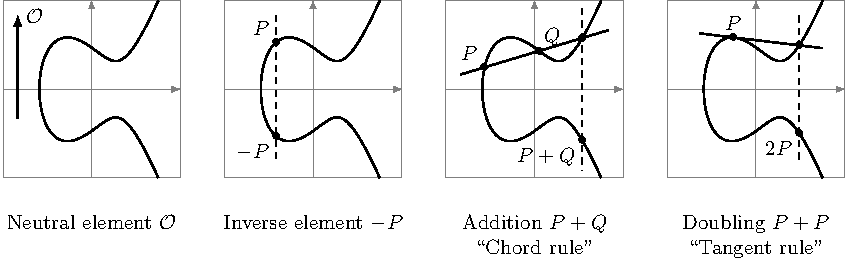
\includegraphics{ecc/ec_group_operations.pdf}
\caption{Geometric Representation of Elliptic Curve Group Operation}
 \label{fig:oper}
\end{figure}

All the points on an elliptic curve form an abelian group. We assume that every vertical line passes through a point called neutral element or point of infinity $ \cal O$ as shown in the \figref{fig:oper}. Inverse element of a point P, $P^{-1}$ is the point of intersection of the vertical line through P and the curve as seen in \figref{fig:oper}. The group operation for Elliptical Curve is called Point Addition and denoted by $P+Q$, where P and Q are points on the curve. Let $\diamond$ operator on points P and Q on the curve represent the intersection point of the line joining P and Q and the curve. Then the point addition can be represented as $\cal O \diamond (P \diamond Q)$. In other words, it represents the intersection of the vertical line through $P \diamond Q$ and the curve depicted in \figref{fig:oper}. The doubling of P, i.e P+P, is represented by similarly by taking the intersection of the tangent at P and the curve and drawing a vertical line through that point to get its intersection with the curve as shown in figure \figref{fig:oper}.

\paragraph{Algebraic Representation.} We can also represent the group operation algebraically for finite fields. The slope for the line between point P(x1,y1) and Q(x2,y2) is $D = \frac{y2-y1}{x2-x1} \mod p$. Thus the equation for the line will be  $y = D(x-x1) + y1 \mod p$. To find the intersection of the line with the curve, we will substitute the value of y to get ${(D(x-x1) + y1)}^2 = x^3 + ax + b \mod p$. The solution of this equation are x1 , x2 and $x3 = D^2-x1-x2 \mod p$, which gives $y3 = D(x3-x1) + y1 \mod p$. The pseudo code to get the Point Addition between two points P and Q is discussed in Algorithm \ref{algo}. The pseudo code also handles the corner cases where the P or Q is $\cal O$, then the result will be the other point as $P+\cal O = P$. In case the points are symmetric, the point addition will return $\cal O$ as $P + P^{-1}=\cal O $. Finally in case of point doubling, the slope with be the slope of the tangent at that point.

\makeatletter
\def\BState{\State\hskip-\ALG@thistlm}
\makeatother

\begin{algorithm}
\caption{PointAddition Algorithm with input P(x1,y1) and Q(x2,y2) }\label{algo}
\begin{algorithmic}[1]
\Procedure{PointAddition}{}
\If {$P = \cal O$}
return Q
\EndIf
\If {$Q = \cal O$}
return P
\EndIf
\If {$x1 = x2$ and $y1 = -y2$}
return $\cal O$
\EndIf
\If{$x1 = x2$ and $y1 = y2$}
\State $D \gets \frac{3*{x1}^2+a}{2*y1} \mod p$
\Else 
\State $D \gets \frac{y2-y1}{x2-x1} \mod p$
\EndIf
\State $x3 \gets D^2-x1-x2 \mod p$
\State $y3 \gets D(x3-x1) + y1 \mod p$
\State return (x3,-y3)
\EndProcedure
\end{algorithmic}
\end{algorithm}

Interestingly, the point addition is an abelian group operation as it satisfies all four properties for group operation plus commutative property.
\begin{itemize}
\item Closure Property. P+Q lies on the curve for all P and Q, as discussed earlier.
\item Associative Property. (P+Q)+R = P+(Q+R)
\item Inverse Property. $P + P^{-1} = \cal O $ where $P^{-1} = (-x,y)$ for P=(x,y). Also ${\cal O}^{-1} = \cal O$. Since line passing through P and $P^{-1}$ is a vertical line, it passes through $\cal O$.
\item Identity Property. P+$\cal O$ = P, as the vertical line intersects the inverse point $P^{-1}$, and vertical line through $P^{-1}$ intersect $P$. Thus the point of infinity is an identity for the group.
\item Commutative Property. P+Q = Q +P, as the line passing through P and Q, will be the same in both cases.
\end{itemize}

\paragraph{Scalar Multiplication.} Scalar multiplication $nP$ is equivalent to adding P to itself n times. This is analogous to exponentiation in $Z_p$ and can be computed by point double and add algorithm similar to square and multiply in case of integers. We can also pick generator P that defines a cyclic subgroup of E such that $0P, 1P, 2P, 3P \dots qP$ all lies on the curve. 

\paragraph{Building Elliptic Curve Groups.} Earlier people used to find suitable curves by a deterministic algorithm that picks a large prime p and random a and b to define a curve. Then we can determine the size of the group in polynomial time using Schoof algorithm. The size of the group should be large and prime for security reasons. Finally, pick a point P on the curve to be a generator. This process was very slow. Recently, these curves and generator point P have been standardized instead. Some examples of such curves are NIST curves, Curve25519. 







\subsection{Elliptic Curve Diffie Hellman}

The Elliptic Curve Group can be used to perform Elliptic Curve Diffie Hellman for key exchange \figref{fig:ecdh}. It is very similar to Diffie Hellman except that it uses group operation instead of exponentiation \figref{fig:dh}. The security needed by Elliptic Curve Diffie Hellman is analogous to Computational Diffie Hellman Assumption that given X and Y one can't learn $xyP$. The best way to solve Elliptic Curve Computational Diffie Hellman is to solve Elliptic Curve Discrete Log Problem which is given X, compute the value of x. One of the generic attacks against the Elliptic Curve Discrete Log Problem is Baby-Step Giant-Step Algorithm.

\begin{figure}[t]
  \centering
  \pseudocode{
    \textbf{Client} \> {} \> \textbf{ Server}\\[2pt][\hline]\\[-0.5\baselineskip]
    x \sample \Z_q \> \> y \sample \Z_q\\
   X = Px \> \> Y=Py\\
    \> \sendmessagerightx[0.5in]{1}{X} \>\\
    \> \sendmessageleftx[0.5in]{1}{Y}\>\\
    K = H(xY) \> \> K = H(yX)
   % \> \sendmessagerightx[0.5in]{1}{b} \> \\
    %\> \> (\mathbf{\typo}, \mathbf{\usernameT}) \leftarrow \textsf{A}(b)\\
    %\> ({\pw,\username})  \xleftrightarrow {\text{Set Intersection}} (\mathbf{\typo}, \mathbf{\usernameT})\\
  }
  \caption{Elliptic Curve Diffie Hellman Key Exchange}
  \label{fig:ecdh}
\end{figure}

\begin{figure}[t]
  \centering
  \pseudocode{
    \textbf{Client} \> {} \> \textbf{ Server}\\[2pt][\hline]\\[-0.5\baselineskip]
    x \sample \Z_q \> \> y \sample \Z_q\\
   X = g^x \> \> Y=g^y\\
    \> \sendmessagerightx[0.5in]{1}{X} \>\\
    \> \sendmessageleftx[0.5in]{1}{Y}\>\\
    K = H(Y^x) \> \> K = H(X^y)
   % \> \sendmessagerightx[0.5in]{1}{b} \> \\
    %\> \> (\mathbf{\typo}, \mathbf{\usernameT}) \leftarrow \textsf{A}(b)\\
    %\> ({\pw,\username})  \xleftrightarrow {\text{Set Intersection}} (\mathbf{\typo}, \mathbf{\usernameT})\\
  }
  \caption{Diffie Hellman Key Exchange }
  \label{fig:dh}
\end{figure}


\paragraph{Baby-Step Giant-Step Algorithm.} Baby-Step Giant-Step algorithm tries to solve the Elliptic Curve Discrete Log Problem, which is given xP for a random x, compute x. The algorithm is shown in \ref{fig:bsgs}. In the algorithm, we take rewrite $x = a*m+b$, then multiplying it by P, we get $xP + (-amP) = bP$. We precompute pairs of (b, bP) for different values of P. Then find the value of a for which $xP + (-amP) = bP$ and the value of x will be then $a*m+b$ for the given a and b. The worst-case runtime of this algorithm $q^{0.5}$. But the space complexity is also $q^{0.5}$. Pollard Rho method reduces the space complexity to constant. This is the best-known attack against Elliptic Curve. This attack can also be used against Discrete Log Problem, by just replacing group operation by exponentiation. There are, however, a bunch of corner cases for some curves where attacks can be faster.


\begin{algorithm}
\caption{Baby-Step Giant-Step Algorithm with input xP,P,q }\label{fig:bsg}
\begin{algorithmic}[1]
\Procedure{BabyStepGiantStep}{}
\State Let $x = a*m+b$ with $m = ceil(q^{0.5})$ then
\State xP + (-amP) = bP
\For{$b = 1 \dots m$}
\State Store(b,bP)
\EndFor
\For{$a = 1 \dots m$}
\If{xP+(-amP) = bP}
\State return am+b
\EndIf
\EndFor
\EndProcedure
\end{algorithmic}
\end{algorithm}

\paragraph{Point Compression.} Any point x has exactly 0 or 2 solutions to the curve equation. Also, the two solutions are symmetric against x-axis. Thus, we can reduce the space to represent the points in Elliptic Curve by just representing x and a bit 0 or 1 to represent y. This reduces the space complexity by a factor of 2.

\subsection{Summary}
Elliptic Curves are specially constructed groups where Discrete Log Problem is conjectured to be hard. These group operations are faster than RSA or Diffie Hellman over $Z_p$. These are increasingly used in practice and are being adopted where Discrete Log Property is required for security, eg Signing Algorithm(EC-DSA algorithm), etc.



\newpage
%%%%%%%%%%%%%%%%%%%%%%%%%%%%%%%%%%%%%%%%%%%%%%%%%%%%%%%%%%%%%%%%%%%%%%%%%%%%%%%%
\section{Public Key Encryption under Chosen-Ciphertext Attacks}
\label{sec:pke}

A PKE scheme $\AEnc = (\kg,\enc,\dec)$ is a triple of
algorithms. Key generation is randomized and outputs a key pair $(\pk,\sk)$.
Encryption
takes as input a public key $\pk$ and message $M$ and outputs a ciphertext.
Decryption takes as input a secret key $\sk$ and ciphertext $C$ and outputs a
message or a distinguished error symbol $\bot$. 


\hfpagess{.15}{.15}{
\underline{$\LORCCA1^\advA_{\SE}$}\\[1pt]
$(\pk,\sk) \getsr \kg$\\
$b' \getsr \advA^{\EncOracle,\DecOracle}(\pk)$\\
Ret $b'$\medskip

\underline{$\EncOracle(M_0,M_1)$}\\
$C \getsr \enc(\pk,M_1)$\\
$\calC \gets \calC \cup \{C\}$\\
Ret $C$\medskip

\underline{$\DecOracle(C)$}\\
If $C \in \calC$ then \\
\myInd Ret $\bot$\\
Ret $\dec(\sk,C)$
}{
\underline{$\LORCCA0^\advA_{\SE}$}\\[1pt]
$(\pk,\sk) \getsr \kg$\\
$b' \getsr \advA^{\EncOracle,\DecOracle}(\pk)$\\
Ret $b'$\medskip

\underline{$\EncOracle(M_0,M_1)$}\\
$C \getsr \enc(\pk,M_0)$\\
$\calC \gets \calC \cup \{C\}$\\
Ret $C$\medskip

\underline{$\DecOracle(C)$}\\
Ret $\bot$
}




\fpage{.20}{
		\underline{$\INDCCA_\AEnc^\advA$}\\
    $(\pk,\sk) \getsr \kg$\\
    $b \getsr \bits$\\
    $b' \getsr \advA^{\EncOracle,\DecOracle}(\pk)$\\
		Ret $(b'=b)$\medskip

    \underline{$\EncOracle(M_0,M_1)$}\\
    If $|M_0| \ne |M_1|$ then\\
    \myInd Ret $\bot$\\
    $C \getsr \enc(\pk,M_b)$\\
    $\calC \gets \calC \cup \{C\}$\\
    Ret $C$\medskip

    \underline{$\DecOracle(C)$}\\
    If $C \in \calC$ then Ret $\bot$\\
    $M \getsr \dec(\sk,C)$\\
    Ret $M$
	}

\begin{align*}
  \AdvINDCCA{\AEnc}{\advA} &= 2\cdotsm\Prob{\INDCCA_\AEnc^\advA\Rightarrow\true} - 1
%        &= \left|\Prob{\INDCCA1_\AEnc^\advA\Rightarrow\true} - \Prob{\INDCCA0_\AEnc^\advA\Rightarrow\false}\right|
\end{align*}


\begin{theorem*}
Let $\RSAk$ be the RSA-based scheme using
security parameter $k$, hash function
$\Horacle\Colon\msgspace\rightarrow\bits^n$ modeled as a random oracle, and
symmetric encryption scheme $\SEscheme$. Let $\advA$ be
an $\INDCCA_{\RSAk}$-adversary making at most $q_H$ queries to
$\Horacle$ and $q_d$ queries to its decyrption oracle. Then we give an
$\OWF_{\RSAk}$-adversary $\advB$ and $\RORCCA_\SEscheme$-adversary
$\advC$ such that
\bnm
  \AdvINDCPA{\RSAk,\Horacle}{\advA} \le
      2\cdotsm\AdvOWF{\RSAk}{\advB} +  
        2\cdotsm\AdvRORCCA{\SEscheme}{\advC}  \;.
\enm
Adversaries $\advB,\advC$ run in time that of $\advA$ plus 
the time to perform simulate $q_H$ exponentations. 
Adversary $\advC$ makes a single encryption query.
\end{theorem*}



\hfpages{.15}{
\underline{$\enc(X,M)$}\\
$r \getsr \Z_{|G|}$\\
$C_0 \gets g^r$\\
$C_1 \gets X^r \cdot M$\\
Ret $(C_0,C_1)$
}{
\underline{$\dec(x,(C_1,C_2))$}\\
$M \gets C_2 \cdotsm C_1^{-x}$\\
Ret $M$
}

\hfpages{.15}{
\underline{$\enc(X,M)$}\\
$r \getsr \Z_{|G|}$\\
$C_0 \gets g^r$\\
$K \gets H(g^r \concat X^r)$\\
$C_1 \gets \enc_s(K,M)$\\
Ret $(C_0,C_1)$
}{
\underline{$\dec(x,(C_1,C_2))$}\\
$K \gets H(C_1\concat C_1^x)$\\
$M \gets \dec_S(K,C_2)$\\
Ret $M$
}

\fpage{.23}{
\underline{$\ICDH_{G,g}^\advB$}\\
$b \getsr \bits$\\
$x,y,z \getsr \Z_{|G|}$\\
$Z_0 \gets g^z$\\
$Z_1 \gets g^{xy}$\\
$b' \getsr \advB^{\DDHoracle}(g,g^x,g^y,Z_b)$\\
Ret $(b' = b)$\medskip

\underline{$\DDHoracle(\hat{Y},\hat{Z})$}\\
If $\hat{Y}^x = \hat{Z}$ then\\
\myInd Ret 1\\
Ret 0
}


\fpage{.20}{
		\underline{$\G_{i^*}$}\\
    $b \getsr \bits$\\
    $(\pk,\sk) \getsr \kg$\\
    $i \gets 1$\\
    $b' \getsr \advA^\EncOracle(\pk)$\\
		Ret $b'$\medskip

    \underline{$\EncSim(M_0,M_1)$}\\
    If $|M_0| \ne |M_1|$ then\\
    \myInd Ret $\bot$\\
    If $i > i^*$ then\\ 
    \myInd $C \getsr \enc(\pk,M_0)$\\
    Else\\
    \myInd $C \getsr \enc(\pk,M_1)$\\
    $i \gets i + 1$\\
    Ret $C$
	}



\fpage{.20}{
		\underline{$\advB^\EncOracle(\pk)$}\\
    $i \gets 1$\\
    $b' \getsr \advA^\EncSim(\pk)$\\
		Ret $b'$\medskip

    \underline{$\EncSim(M_0,M_1)$}\\
    If $|M_0| \ne |M_1|$ then\\
    \myInd Ret $\bot$\\
    If $i > i^*$ then\\ 
    \myInd $C \getsr \enc(\pk,M_1)$\\
    Else if $i = i^*$ then\\
    \myInd $C \gets \EncOracle(M_0,M_1)$\\
    Else\\
    \myInd $C \getsr \enc(\pk,M_0)$\\
    $i \gets i + 1$\\
    Ret $C$
	}


\begin{align*}
\AdvINDCPA{\AEnc}{\advA} 
  &= \left|\Prob{\G_0\Rightarrow1} - \Prob{\G_1\Rightarrow1}\right|\\
  &= \left|\sum_{i=1}^q \Prob{\G_{i-1}\Rightarrow1} - \Prob{\G_i\Rightarrow1}\right| \\
  &= \left|\sum_{i=1}^q 
      \Prob{\INDCPA1^{\advB_i}_\AEnc\Rightarrow 1}
      - \Prob{\INDCPA0^{\advB_i}_\AEnc\Rightarrow 1}\right|
\end{align*}

\begin{align*}
  \AdvINDCPA{\AEnc}{\advB}
    &= \left| \Prob{\INDCPA1^\advB\Rightarrow1} - \Prob{\INDCPA0^\advB\Rightarrow1} \right|\\
    &= \frac{1}{q} \left|
    \sum_{i^*=1}^q\CondProb{\INDCPA1^\advB\Rightarrow1}{j= i^*} -
    \CondProb{\INDCPA0^\advB\Rightarrow1}{j=i^*} \right|\\
    &= \frac{1}{q} \left|
    \sum_{i^*=1}^q\Prob{\INDCPA1^{\advB_{i^*}}\Rightarrow1} - \Prob{\INDCPA0^{\advB_{i^*}}\Rightarrow1} \right|
\end{align*}
  

\begin{align*}
\AdvINDCPA{\AEnc}{\advB} 
  &= \left|\Prob{\INDCPA0_\AEnc^\advB\Rightarrow1} -
                      \Prob{\INDCPA1_\AEnc^\advB\Rightarrow1}\right|\\
  &= \frac{1}{q}\sum_{i=0}^{q-1} \left|\Prob{\G_i\Rightarrow1} - \Prob{\G_{i+1}\Rightarrow1}\right|\\
  &= \frac{1}{q}\left|\Prob{\G_0\Rightarrow1} - \Prob{\G_q\Rightarrow1}\right|
\end{align*}


\fpage{.20}{
		\underline{$\OWF_{\RSAk}$}\\
    $((N,e),(N,d))\getsr \kg(k)$\\
    $X \getsr \Z_N^*$\\
    $Y \gets X^e \bmod N$\\
    $X' \getsr \advA(Y)$\\
		Ret $(X' = X)$
	}

\bnm
  \AdvOWFRSA{\RSAk}{\advA} = \Prob{\OWF_{\RSAk}^\advA\Rightarrow\true}
\enm


\begin{theorem*}
Let $\RSAk$ be the RSA-based scheme using
security parameter $k$, hash function
$\Horacle\Colon\msgspace\rightarrow\bits^n$ modeled as a random oracle, and
symmetric encryption scheme $\SEscheme$. Let $\advA$ be
an $\INDCPA_{\RSAk}$-adversary making at most $q$ queries to
$\Horacle$. Then we give an
$\OWF_{\RSAk}$-adversary $\advB$ and $\INDCPA_\SEscheme$-adversary
$\advC$ such that
\bnm
  \AdvINDCPA{\RSAk,\Horacle}{\advA} \le
      2\cdotsm\AdvOWF{\RSAk}{\advB} +  
        2\cdotsm\AdvROR{\SEscheme}{\advC}  \;.
\enm
Adversaries $\advB,\advC$ run in time that of $\advA$ plus 
the time to simulate $q$ RO queries. Adversary $\advC$ makes a single encryption query.
\end{theorem*}


\hfpagesss{.20}{.20}{.20}{
\underline{$\G_0$}\\
$b \getsr \bits$\\
$((N,e),(N,d)) \getsr \kg(k)$\\
$b' \getsr \advA^{\EncOracle,\Horacle}(N,e)$\\
Ret $b'$\medskip

\underline{$\EncOracle(M_0,M_1)$}\\
$R \getsr \Z^*_N$\\
$C_1 \gets R^e \bmod N$\\
$K \gets \Horacle(R)$\\
$C_2 \getsr \encSym(K,M)$\\
Ret $(C_1,C_2)$\medskip

\underline{$\Horacle(X)$}\\
If $\TabH[X] = \bot$  then\\
\myInd $\TabH[X] \getsr \bits^n$\\
Ret $\TabH[X]$
}{
\underline{\fbox{$\G_1$}\;\;\; $\G_2$}\\
$((N,e),(N,d)) \getsr \kg(k)$\\
$R \getsr \Z^*_N$\\
$C_1 \gets R^e \bmod N$\\
$K \getsr \bits^n$\\
$b \getsr \bits$\\
$b' \getsr \advA^{\EncOracle,\Horacle}(N,e)$\\
Ret $b'$\medskip

\underline{$\EncOracle(M_0,M_1)$}\\
$C_2 \getsr \encSym(K,M)$\\
Ret $(C_1,C_2)$\medskip

\underline{$\Horacle(X)$}\\
If $X = R$ then\\
\myInd $\badtrue$\\
\myInd \fbox{$\TabH[X] \gets K$}\\
If $\TabH[X] = \bot$  then\\
\myInd $\TabH[X] \getsr \bits^n$\\
Ret $\TabH[X]$
}{
\underline{$\G_3$}\\
$((N,e),(N,d)) \getsr \kg(k)$\\
$R \getsr \Z^*_N$\\
$C_1 \gets R^e \bmod N$\\
$K \getsr \bits^n$\\
$b \getsr \bits$\\
$b' \getsr \advA^{\EncOracle,\Horacle}(N,e)$\\
Ret $b'$\medskip

\underline{$\EncOracle(M_0,M_1)$}\\
%$C_2 \getsr \encSym(K,M)$\\
$C_2 \getsr \bits^{\ctxtlen(M_0)}$\\
Ret $(C_1,C_2)$\medskip

\underline{$\Horacle(X)$}\\
If $\TabH[X] = \bot$  then\\
\myInd $\TabH[X] \getsr \bits^n$\\
Ret $\TabH[X]$
}




\hfpages{.2}{
		\underline{$\enc((N,e),M)$:}\\
    $R \getsr \Z^*_N$\\
    $C_1 \gets R^e \bmod N$\\
    $K \gets H(R)$\\
    $C_2 \getsr \encSym(K,M)$\\
		Ret $(C_1,C_2)$
  }{
	  \underline{$\dec((N,d),(C_1,C_2))$:}\\
    $R \gets C_1^d \bmod N$\\
    $K \gets H(R)$\\
    $M \gets \decSym(K,C_2)$\\
		Ret $M$
	}

$\SEscheme = (\kgSym,\encSym,\decSym)$


\hfpages{.15}{
\underline{$\enc(X,M)$}\\
$r \getsr \Z_{|G|}$\\
$C_0 \gets g^r$\\
$C_1 \gets X^r \cdot M$\\
Ret $(C_0,C_1)$
}{
\underline{$\dec(x,(C_1,C_2))$}\\
$M \gets C_2 \cdotsm C_1^{-x}$\\
Ret $M$
}


\fpage{.20}{
\underline{$\DDH_{G,g}^\advB$}\\
$b \getsr \bits$\\
$x,y,z \getsr \Z_{|G|}$\\
$Z_0 \gets g^z$\\
$Z_1 \gets g^{xy}$\\
$b' \getsr \advB(g,g^x,g^y,Z_b)$\\
Ret $(b' = b)$
}

\begin{theorem}
Let $\AEnc$ be the El Gamal scheme over group $G$ with generator $g$. 
Let $\advA$ be an $\INDCPA_\AEnc$-adversary. Then we give a $\DDH_{G,g}$ 
adversary $\advB$ such that 
\bnm
  \AdvINDCPA{\AEnc}{\advA} \le 2\cdotsm \AdvDDH{G,g}{\advB} \;.
\enm
Adversary $\advB$ runs in time that of $\advA$. 
\end{theorem}


\fpage{.20}{
\underline{$G_0$ \;\;\; \fbox{$G_1$}}\\
$b \getsr \bits$\\
$x \getsr \Z_{|G|}$\\
$X \gets g^x$\\
$b' \getsr \advA^\EncOracle(g,X)$\\
Ret $(b' = b)$\medskip

\underline{$\EncOracle(M_0,M_1)$}\\
$C_1 \gets g^y$\\
$Z \gets g^{xy}$\\
\fbox{$z \getsr \Z_{|G|}$ \;;\; $Z \gets g^z$}\\
$C_2 \gets Z\cdot M_b$\\
Ret $(C_1,C_2)$
}

\fpage{.20}{
\underline{Adversary $\advB(X,Y,Z)$}\\
$b \getsr \bits$\\
$b' \getsr \advA^\EncSim(g,X)$\\
Ret $(b' = b)$\medskip

\underline{$\EncSim(M_0,M_1)$}\\
$C_1 \gets Y$\\
$C_2 \gets Z\cdot M_b$\\
Ret $(C_1,C_2)$
}


\begin{align*}
  \AdvINDCPA{\AEnc}{\advA} 
    &= 2\cdotsm\Prob{\INDCPA_{\AEnc}^\advA\Rightarrow\true} - 1\\
    &= 2\cdotsm\Prob{G_0\Rightarrow\true} - 1\\
    &= 2\cdotsm\left(\Prob{G_1\Rightarrow\true} + \AdvDDH{G,g}{\advB})\right) - 1\\
    &= 2\cdotsm\left(\frac{1}{2}+ \AdvDDH{G,g}{\advB})\right) - 1
\end{align*}



\bnm
J_p(a) = \left\{ \begin{array}{rl} 
            1 & \textnormal{if $a$ is square mod $p$}\\
            0 & \textnormal{if $a \bmod p = 0$}\\
            -1 & \textnormal{otherwise}
      \end{array}\right.
\enm


\fpage{.20}{
\underline{Adversary $\advB(X,Y,Z)$}\\
If $J_p(X) = 1$ or $J_p(Y) = 1$ then\\
\myInd $s \gets 1$\\
Else \\
\myInd $s \gets -1$\\
If $J_p(Z) = s$ then\\
\myInd Ret 1
Ret 0
}


\newpage
\huge
% Graphic for TeX using PGF
% Title: /home/phil/digsigs.dia
% Creator: Dia v0.97+git
% CreationDate: Mon Apr 22 16:47:42 2019
% For: phil
% \usepackage{tikz}
% The following commands are not supported in PSTricks at present
% We define them conditionally, so when they are implemented,
% this pgf file will use them.
\ifx\du\undefined
  \newlength{\du}
\fi
\setlength{\du}{15\unitlength}
\begin{tikzpicture}[even odd rule]
\pgftransformxscale{1.000000}
\pgftransformyscale{-1.000000}
\definecolor{dialinecolor}{rgb}{0.000000, 0.000000, 0.000000}
\pgfsetstrokecolor{dialinecolor}
\pgfsetstrokeopacity{1.000000}
\definecolor{diafillcolor}{rgb}{1.000000, 1.000000, 1.000000}
\pgfsetfillcolor{diafillcolor}
\pgfsetfillopacity{1.000000}
\pgfsetlinewidth{0.100000\du}
\pgfsetdash{}{0pt}
\pgfsetbuttcap
\pgfsetmiterjoin
\pgfsetlinewidth{0.100000\du}
\pgfsetbuttcap
\pgfsetmiterjoin
\pgfsetdash{}{0pt}
{\pgfsetcornersarced{\pgfpoint{0.000000\du}{0.000000\du}}\definecolor{diafillcolor}{rgb}{0.000000, 0.792157, 0.839216}
\pgfsetfillcolor{diafillcolor}
\pgfsetfillopacity{1.000000}
\fill (7.782258\du,3.700000\du)--(7.782258\du,7.750000\du)--(11.701613\du,7.750000\du)--(11.701613\du,3.700000\du)--cycle;
}{\pgfsetcornersarced{\pgfpoint{0.000000\du}{0.000000\du}}\definecolor{dialinecolor}{rgb}{0.000000, 0.000000, 0.000000}
\pgfsetstrokecolor{dialinecolor}
\pgfsetstrokeopacity{1.000000}
\draw (7.782258\du,3.700000\du)--(7.782258\du,7.750000\du)--(11.701613\du,7.750000\du)--(11.701613\du,3.700000\du)--cycle;
}% setfont left to latex
\definecolor{dialinecolor}{rgb}{0.000000, 0.000000, 0.000000}
\pgfsetstrokecolor{dialinecolor}
\pgfsetstrokeopacity{1.000000}
\definecolor{diafillcolor}{rgb}{0.000000, 0.000000, 0.000000}
\pgfsetfillcolor{diafillcolor}
\pgfsetfillopacity{1.000000}
\node[anchor=base west,inner sep=0pt,outer sep=0pt,color=dialinecolor] at (9.000000\du,6.000000\du){kg};
\pgfsetlinewidth{0.100000\du}
\pgfsetdash{}{0pt}
\pgfsetbuttcap
\pgfsetmiterjoin
\pgfsetlinewidth{0.100000\du}
\pgfsetbuttcap
\pgfsetmiterjoin
\pgfsetdash{}{0pt}
{\pgfsetcornersarced{\pgfpoint{0.000000\du}{0.000000\du}}\definecolor{diafillcolor}{rgb}{0.000000, 0.792157, 0.839216}
\pgfsetfillcolor{diafillcolor}
\pgfsetfillopacity{1.000000}
\fill (2.782258\du,11.700000\du)--(2.782258\du,15.750000\du)--(6.701613\du,15.750000\du)--(6.701613\du,11.700000\du)--cycle;
}{\pgfsetcornersarced{\pgfpoint{0.000000\du}{0.000000\du}}\definecolor{dialinecolor}{rgb}{0.000000, 0.000000, 0.000000}
\pgfsetstrokecolor{dialinecolor}
\pgfsetstrokeopacity{1.000000}
\draw (2.782258\du,11.700000\du)--(2.782258\du,15.750000\du)--(6.701613\du,15.750000\du)--(6.701613\du,11.700000\du)--cycle;
}% setfont left to latex
\definecolor{dialinecolor}{rgb}{0.000000, 0.000000, 0.000000}
\pgfsetstrokecolor{dialinecolor}
\pgfsetstrokeopacity{1.000000}
\definecolor{diafillcolor}{rgb}{0.000000, 0.000000, 0.000000}
\pgfsetfillcolor{diafillcolor}
\pgfsetfillopacity{1.000000}
\node[anchor=base west,inner sep=0pt,outer sep=0pt,color=dialinecolor] at (3.596369\du,13.946183\du){sign};
\pgfsetlinewidth{0.100000\du}
\pgfsetdash{}{0pt}
\pgfsetbuttcap
\pgfsetmiterjoin
\pgfsetlinewidth{0.100000\du}
\pgfsetbuttcap
\pgfsetmiterjoin
\pgfsetdash{}{0pt}
{\pgfsetcornersarced{\pgfpoint{0.000000\du}{0.000000\du}}\definecolor{diafillcolor}{rgb}{0.000000, 0.792157, 0.839216}
\pgfsetfillcolor{diafillcolor}
\pgfsetfillopacity{1.000000}
\fill (13.782258\du,11.700000\du)--(13.782258\du,15.750000\du)--(17.701613\du,15.750000\du)--(17.701613\du,11.700000\du)--cycle;
}{\pgfsetcornersarced{\pgfpoint{0.000000\du}{0.000000\du}}\definecolor{dialinecolor}{rgb}{0.000000, 0.000000, 0.000000}
\pgfsetstrokecolor{dialinecolor}
\pgfsetstrokeopacity{1.000000}
\draw (13.782258\du,11.700000\du)--(13.782258\du,15.750000\du)--(17.701613\du,15.750000\du)--(17.701613\du,11.700000\du)--cycle;
}% setfont left to latex
\definecolor{dialinecolor}{rgb}{0.000000, 0.000000, 0.000000}
\pgfsetstrokecolor{dialinecolor}
\pgfsetstrokeopacity{1.000000}
\definecolor{diafillcolor}{rgb}{0.000000, 0.000000, 0.000000}
\pgfsetfillcolor{diafillcolor}
\pgfsetfillopacity{1.000000}
\node[anchor=base west,inner sep=0pt,outer sep=0pt,color=dialinecolor] at (14.838548\du,14.000000\du){ver};
% setfont left to latex
\definecolor{dialinecolor}{rgb}{0.000000, 0.000000, 0.000000}
\pgfsetstrokecolor{dialinecolor}
\pgfsetstrokeopacity{1.000000}
\definecolor{diafillcolor}{rgb}{0.000000, 0.000000, 0.000000}
\pgfsetfillcolor{diafillcolor}
\pgfsetfillopacity{1.000000}
\node[anchor=base west,inner sep=0pt,outer sep=0pt,color=dialinecolor] at (7.000000\du,11.200000\du){sk};
% setfont left to latex
\definecolor{dialinecolor}{rgb}{0.000000, 0.000000, 0.000000}
\pgfsetstrokecolor{dialinecolor}
\pgfsetstrokeopacity{1.000000}
\definecolor{diafillcolor}{rgb}{0.000000, 0.000000, 0.000000}
\pgfsetfillcolor{diafillcolor}
\pgfsetfillopacity{1.000000}
\node[anchor=base west,inner sep=0pt,outer sep=0pt,color=dialinecolor] at (12.100000\du,11.200000\du){pk};
% setfont left to latex
\definecolor{dialinecolor}{rgb}{0.000000, 0.000000, 0.000000}
\pgfsetstrokecolor{dialinecolor}
\pgfsetstrokeopacity{1.000000}
\definecolor{diafillcolor}{rgb}{0.000000, 0.000000, 0.000000}
\pgfsetfillcolor{diafillcolor}
\pgfsetfillopacity{1.000000}
\node[anchor=base west,inner sep=0pt,outer sep=0pt,color=dialinecolor] at (7.000000\du,10.000000\du){};
% setfont left to latex
\definecolor{dialinecolor}{rgb}{0.000000, 0.000000, 0.000000}
\pgfsetstrokecolor{dialinecolor}
\pgfsetstrokeopacity{1.000000}
\definecolor{diafillcolor}{rgb}{0.000000, 0.000000, 0.000000}
\pgfsetfillcolor{diafillcolor}
\pgfsetfillopacity{1.000000}
\node[anchor=base west,inner sep=0pt,outer sep=0pt,color=dialinecolor] at (11.178686\du,12.978978\du){M};
% setfont left to latex
\definecolor{dialinecolor}{rgb}{0.000000, 0.000000, 0.000000}
\pgfsetstrokecolor{dialinecolor}
\pgfsetstrokeopacity{1.000000}
\definecolor{diafillcolor}{rgb}{0.000000, 0.000000, 0.000000}
\pgfsetfillcolor{diafillcolor}
\pgfsetfillopacity{1.000000}
\node[anchor=base west,inner sep=0pt,outer sep=0pt,color=dialinecolor] at (0.414624\du,14.186366\du){M};
% setfont left to latex
\definecolor{dialinecolor}{rgb}{0.000000, 0.000000, 0.000000}
\pgfsetstrokecolor{dialinecolor}
\pgfsetstrokeopacity{1.000000}
\definecolor{diafillcolor}{rgb}{0.000000, 0.000000, 0.000000}
\pgfsetfillcolor{diafillcolor}
\pgfsetfillopacity{1.000000}
\node[anchor=base west,inner sep=0pt,outer sep=0pt,color=dialinecolor] at (11.357372\du,15.147153\du){$\sigma$};
% setfont left to latex
\definecolor{dialinecolor}{rgb}{0.000000, 0.000000, 0.000000}
\pgfsetstrokecolor{dialinecolor}
\pgfsetstrokeopacity{1.000000}
\definecolor{diafillcolor}{rgb}{0.000000, 0.000000, 0.000000}
\pgfsetfillcolor{diafillcolor}
\pgfsetfillopacity{1.000000}
\node[anchor=base west,inner sep=0pt,outer sep=0pt,color=dialinecolor] at (11.000000\du,15.000000\du){};
% setfont left to latex
\definecolor{dialinecolor}{rgb}{0.000000, 0.000000, 0.000000}
\pgfsetstrokecolor{dialinecolor}
\pgfsetstrokeopacity{1.000000}
\definecolor{diafillcolor}{rgb}{0.000000, 0.000000, 0.000000}
\pgfsetfillcolor{diafillcolor}
\pgfsetfillopacity{1.000000}
\node[anchor=base west,inner sep=0pt,outer sep=0pt,color=dialinecolor] at (8.078040\du,14.141215\du){$\sigma$};
% setfont left to latex
\definecolor{dialinecolor}{rgb}{0.000000, 0.000000, 0.000000}
\pgfsetstrokecolor{dialinecolor}
\pgfsetstrokeopacity{1.000000}
\definecolor{diafillcolor}{rgb}{0.000000, 0.000000, 0.000000}
\pgfsetfillcolor{diafillcolor}
\pgfsetfillopacity{1.000000}
\node[anchor=base west,inner sep=0pt,outer sep=0pt,color=dialinecolor] at (19.161144\du,14.098928\du){0/1};
\pgfsetlinewidth{0.100000\du}
\pgfsetdash{}{0pt}
\pgfsetmiterjoin
\pgfsetbuttcap
{
\definecolor{diafillcolor}{rgb}{0.000000, 0.000000, 0.000000}
\pgfsetfillcolor{diafillcolor}
\pgfsetfillopacity{1.000000}
% was here!!!
{\pgfsetcornersarced{\pgfpoint{0.000000\du}{0.000000\du}}\definecolor{dialinecolor}{rgb}{0.000000, 0.000000, 0.000000}
\pgfsetstrokecolor{dialinecolor}
\pgfsetstrokeopacity{1.000000}
\draw (9.703125\du,7.849999\du)--(9.761189\du,7.849999\du)--(9.761189\du,9.499999\du)--(7.561189\du,9.499999\du);
}}
\pgfsetlinewidth{0.100000\du}
\pgfsetdash{}{0pt}
\pgfsetmiterjoin
\pgfsetbuttcap
{
\definecolor{diafillcolor}{rgb}{0.000000, 0.000000, 0.000000}
\pgfsetfillcolor{diafillcolor}
\pgfsetfillopacity{1.000000}
% was here!!!
{\pgfsetcornersarced{\pgfpoint{0.000000\du}{0.000000\du}}\definecolor{dialinecolor}{rgb}{0.000000, 0.000000, 0.000000}
\pgfsetstrokecolor{dialinecolor}
\pgfsetstrokeopacity{1.000000}
\draw (9.850000\du,7.800000\du)--(9.813065\du,7.800000\du)--(9.813065\du,9.500000\du)--(12.850000\du,9.500000\du);
}}
\pgfsetlinewidth{0.100000\du}
\pgfsetdash{}{0pt}
\pgfsetbuttcap
{
\definecolor{diafillcolor}{rgb}{0.000000, 0.000000, 0.000000}
\pgfsetfillcolor{diafillcolor}
\pgfsetfillopacity{1.000000}
% was here!!!
\pgfsetarrowsend{stealth}
\definecolor{dialinecolor}{rgb}{0.000000, 0.000000, 0.000000}
\pgfsetstrokecolor{dialinecolor}
\pgfsetstrokeopacity{1.000000}
\draw (7.544724\du,9.449766\du)--(7.546334\du,10.279173\du);
}
\pgfsetlinewidth{0.100000\du}
\pgfsetdash{}{0pt}
\pgfsetbuttcap
{
\definecolor{diafillcolor}{rgb}{0.000000, 0.000000, 0.000000}
\pgfsetfillcolor{diafillcolor}
\pgfsetfillopacity{1.000000}
% was here!!!
\pgfsetarrowsend{stealth}
\definecolor{dialinecolor}{rgb}{0.000000, 0.000000, 0.000000}
\pgfsetstrokecolor{dialinecolor}
\pgfsetstrokeopacity{1.000000}
\draw (12.800000\du,9.500000\du)--(12.800000\du,10.300000\du);
}
\pgfsetlinewidth{0.100000\du}
\pgfsetdash{}{0pt}
\pgfsetmiterjoin
\pgfsetbuttcap
{
\definecolor{diafillcolor}{rgb}{0.000000, 0.000000, 0.000000}
\pgfsetfillcolor{diafillcolor}
\pgfsetfillopacity{1.000000}
% was here!!!
\pgfsetarrowsend{stealth}
{\pgfsetcornersarced{\pgfpoint{0.000000\du}{0.000000\du}}\definecolor{dialinecolor}{rgb}{0.000000, 0.000000, 0.000000}
\pgfsetstrokecolor{dialinecolor}
\pgfsetstrokeopacity{1.000000}
\draw (7.000000\du,10.500000\du)--(4.741935\du,10.500000\du)--(4.741935\du,11.700000\du);
}}
\pgfsetlinewidth{0.100000\du}
\pgfsetdash{}{0pt}
\pgfsetmiterjoin
\pgfsetbuttcap
{
\definecolor{diafillcolor}{rgb}{0.000000, 0.000000, 0.000000}
\pgfsetfillcolor{diafillcolor}
\pgfsetfillopacity{1.000000}
% was here!!!
\pgfsetarrowsend{stealth}
{\pgfsetcornersarced{\pgfpoint{0.000000\du}{0.000000\du}}\definecolor{dialinecolor}{rgb}{0.000000, 0.000000, 0.000000}
\pgfsetstrokecolor{dialinecolor}
\pgfsetstrokeopacity{1.000000}
\draw (13.500000\du,10.500000\du)--(15.741935\du,10.500000\du)--(15.741935\du,11.700000\du);
}}
\pgfsetlinewidth{0.100000\du}
\pgfsetdash{}{0pt}
\pgfsetbuttcap
{
\definecolor{diafillcolor}{rgb}{0.000000, 0.000000, 0.000000}
\pgfsetfillcolor{diafillcolor}
\pgfsetfillopacity{1.000000}
% was here!!!
\pgfsetarrowsend{stealth}
\definecolor{dialinecolor}{rgb}{0.000000, 0.000000, 0.000000}
\pgfsetstrokecolor{dialinecolor}
\pgfsetstrokeopacity{1.000000}
\draw (1.461460\du,13.724458\du)--(2.782258\du,13.725000\du);
}
\pgfsetlinewidth{0.100000\du}
\pgfsetdash{}{0pt}
\pgfsetbuttcap
{
\definecolor{diafillcolor}{rgb}{0.000000, 0.000000, 0.000000}
\pgfsetfillcolor{diafillcolor}
\pgfsetfillopacity{1.000000}
% was here!!!
\pgfsetarrowsend{stealth}
\definecolor{dialinecolor}{rgb}{0.000000, 0.000000, 0.000000}
\pgfsetstrokecolor{dialinecolor}
\pgfsetstrokeopacity{1.000000}
\draw (17.701613\du,13.725000\du)--(19.079325\du,13.728557\du);
}
\pgfsetlinewidth{0.100000\du}
\pgfsetdash{}{0pt}
\pgfsetbuttcap
{
\definecolor{diafillcolor}{rgb}{0.000000, 0.000000, 0.000000}
\pgfsetfillcolor{diafillcolor}
\pgfsetfillopacity{1.000000}
% was here!!!
\pgfsetarrowsend{stealth}
\definecolor{dialinecolor}{rgb}{0.000000, 0.000000, 0.000000}
\pgfsetstrokecolor{dialinecolor}
\pgfsetstrokeopacity{1.000000}
\draw (6.701613\du,13.725000\du)--(7.991503\du,13.720273\du);
}
\pgfsetlinewidth{0.100000\du}
\pgfsetdash{}{0pt}
\pgfsetbuttcap
{
\definecolor{diafillcolor}{rgb}{0.000000, 0.000000, 0.000000}
\pgfsetfillcolor{diafillcolor}
\pgfsetfillopacity{1.000000}
% was here!!!
\pgfsetarrowsend{stealth}
\definecolor{dialinecolor}{rgb}{0.000000, 0.000000, 0.000000}
\pgfsetstrokecolor{dialinecolor}
\pgfsetstrokeopacity{1.000000}
\draw (12.509534\du,12.538433\du)--(13.799424\du,12.533705\du);
}
\pgfsetlinewidth{0.100000\du}
\pgfsetdash{}{0pt}
\pgfsetbuttcap
{
\definecolor{diafillcolor}{rgb}{0.000000, 0.000000, 0.000000}
\pgfsetfillcolor{diafillcolor}
\pgfsetfillopacity{1.000000}
% was here!!!
\pgfsetarrowsend{stealth}
\definecolor{dialinecolor}{rgb}{0.000000, 0.000000, 0.000000}
\pgfsetstrokecolor{dialinecolor}
\pgfsetstrokeopacity{1.000000}
\draw (12.414935\du,14.693178\du)--(13.704826\du,14.688451\du);
}
% setfont left to latex
\definecolor{dialinecolor}{rgb}{0.000000, 0.000000, 0.000000}
\pgfsetstrokecolor{dialinecolor}
\pgfsetstrokeopacity{1.000000}
\definecolor{diafillcolor}{rgb}{0.000000, 0.000000, 0.000000}
\pgfsetfillcolor{diafillcolor}
\pgfsetfillopacity{1.000000}
\node[anchor=base west,inner sep=0pt,outer sep=0pt,color=dialinecolor] at (7.311227\du,3.287261\du){\large key generation};
\end{tikzpicture}

\normalsize
\newpage
%%%%%%%%%%%%%%%%%%%%%%%%%%%%%%%%%%%%%%%%%%%%%%%%%%%%%%%%%%%%%%%%%%%%%%%%%%%%%%%%
\section{Identification Protocols and Fiat-Shamir}
\label{sec:idprots}


For our purposes, an identification protocol is a tuple of algorithms
$(\IDkeygen,\IDcom,\IDresp,\IDver)$ and a set $\IDchalset$ called the challenge space. 
The key generation $\IDkeygen$ outputs a public key and secret key pair
$(\pk,\sk)$. The commitment generator $\IDcom$ is randomized and takes the
public key $\pk$ as input. It outputs a commitment. The response generator $\IDresp$ is
deterministic, takes as input the secret key $\sk$, the commitment $R$, and the
challenge $c \in \IDchalset$, and outputs a response~$z$. The verification
algorithm $\IDver$ is deterministic, takes as input a public key $\pk$, 
commitment $R$, challenge $c$, and response $z$, and outputs a bit.  

\bnm
\AdvIDPASS{\IDscheme,q_{id}}{\advA} = \Prob{\IDPASS_{\IDscheme,q_{id}}^\advA\Rightarrow\true}
\enm

\fpage{.40}{
\underline{$\IDPASS_{\IDscheme,q_{id}}^\advA$}\\[1pt]
$(\pk,\sk)\getsr \IDkg$\\
$\queried \gets \false$\\
For $i = 1$ to $q_{id}$ do\\
\myInd $R_i \getsr \IDcom(\pk)$\\
\myInd $c_i \getsr \IDchalset$\\
\myInd $z_i \getsr \IDresp(\sk,R,c)$\\
$z^* \getsr \advA^{\VerOracle}(\pk,(R_1,c_1,z_1),\ldots,(R_{q_{id}},c_{q_{id}},z_{q_{id}}))$\\
Ret $\IDver(\pk,R^*,c^*,z^*)$\medskip

\underline{$\VerOracle(R^*)$}\\[1pt]
If $\queried = \true$ then Ret $\bot$\\
$\queried \gets \true$\\
$c^*\getsr \IDchalset$\\
Ret $c^*$
}


\fpage{.43}{
\underline{$\advB(X)$}\\[1pt]
$\queried \gets \false$\\
For $i = 1$ to $q_{id}$ do\\
\myInd $z_i \getsr \Z_q$\\
\myInd $c_i \getsr \Z_q$\\
\myInd $R_i \getsr g^zX^{-c}$\\
$\coins \getsr \CoinSpace_\advA$\\
$z^* \gets \advA^{\VerOracle}(\pk,(R_1,c_1,z_1),\ldots,(R_{q_{id}},c_{q_{id}},z_{q_{id}}) \semi \coins)$\\
$z^{**} \gets \advA^{\VerOracle}(\pk,(R_1,c_1,z_1),\ldots,(R_{q_{id}},c_{q_{id}},z_{q_{id}}) \semi \coins)$\\
If $c^* = c^{**}$ then Ret $x \getsr \Z_q$\\
$x \gets (z^* - z^{**}) / (c^* - c^{**})$\\
Ret $x$\medskip

\underline{$\VerOracle(R^*)$}\\[1pt]
If $\queried = \false$ then \\
\myInd $\queried \gets \true$\\
\myInd Ret $c^{*} \getsr \Z_q$\\
Ret $c^{**} \getsr \Z_q$
}


\begin{lemma*}
Let $S$ and $T$ be finite, non-empty sets and let $f\Colon S\times T\rightarrow
\bits$ be a function. Let $\calX,\calY,\calY'$ be independent random variables,
with $\calX$ taking values in $T$ and $\calY,\calY'$ being uniformly chosen from
$T$. Let $\Pr[f(\calX,\calY) = 1] = \epsilon$. Then 
\bnm
  \Prob{f(\calX,\calY) = 1 \land f(\calX,\calY') = 1 \land \calY \ne \calY'} 
      \ge \epsilon^2 - \frac{\epsilon}{|T|}
\enm
\end{lemma*}

\begin{proof}[Sketch]
Let $\epsilon(s) = \Pr[f(s,\calY) = 1]$. 
Then $\Ex[\epsilon(\calX)] = \epsilon$. Let $N_s$ be the number of values
$Y \in T$ such that $f(s,Y) = 1$. Let $\calU_s$ be the event that $f(s,\calY) =
1 \land f(s,\calY') = 1 \land \calY \ne \calY'$. Then
\bnm
  \Prob{\calU_s} = \frac{N_s(N_s - 1)}{|T|^2} = \epsilon(s)^2 - \frac{\epsilon(s)}{|T|} 
\enm
Let $\calU$ be event that $f(\calX,\calY) = 1 \land f(\calX,\calY') = 1 \land
\calY \ne \calY'$. Then 
\begin{align*}
  \Prob{\calU} 
  %& =\sum_{s \in S} \Prob{f(\calX,\calY) = 1 \land f(\calX,\calY') = 1 \land \calY \ne \calY' \land \calX = s}\\
  & = \sum_{s \in S} \Prob{f(s,\calY) = 1 \land f(s,\calY') = 1 \land \calY \ne \calY' \land \calX = s}\\
  & = \sum_{s \in S} \Prob{f(s,\calY) = 1 \land f(s,\calY') = 1 \land \calY \ne \calY'}\Prob{\calX = s}\\
  & = \sum_{s \in S} \Prob{\calU_s} \Prob{\calX = s}\\
  & = \sum_{s \in S} \left(\epsilon(s)^2 - \frac{\epsilon(s)}{|T|}\right) \Prob{\calX = s}\\
  & = \Ex[\epsilon(\calX)^2] - \frac{\Ex[\epsilon(\calX)]}{|T|}\\
  & \ge \Ex[\epsilon(\calX)]^2 - \frac{\Ex[\epsilon(\calX)]}{|T|}\\
  & = \epsilon^2 - \frac{\epsilon}{|T|}
\end{align*}
\end{proof}



\begin{theorem*}
Let $G$ be a cyclic group, $q_{id} \ge 0$, 
and $\advA$ be an $\IDPASS_{\IDscheme,q_{id}}$-adversary for the Schnorr
scheme~$\IDscheme$
built using $G$. Then we give an $\DL_G$-adversary $\advB$ such that
\bnm
  \AdvIDPASS{\IDscheme,q_{id}}{\advA} \le \sqrt{\AdvDL{G}{\advB}} + \frac{1}{|G|} \;.
\enm
Adversary~$\advB$ runs in time at most twice that of $\advA$ plus
$\bigO(q_{id})$.
\end{theorem*}


\begin{theorem*}
Let $G$ be a cyclic group and $\DS$ be the Schnorr digital signature scheme
using random oracle $\Horacle \Colon\msgspace\rightarrow\Z_{|G|}$.  
Let $\advA$ be an $\UFCMA_{\DS}$-adversary making at most $q_h$ RO queries and
$q_s$ signing queries.
Then we give an $\DL_G$-adversary $\advB$ such that
\bnm
  \AdvUFCMA{\DS}{\advA} \le \frac{q_s(q_s+q_h+1)}{|G|} + (q_h+1)\left(\sqrt{\AdvDL{G}{\advB}} + \frac{1}{|G|}\right) \;.
\enm
Adversary~$\advB$ runs in time at most twice that of the sum of the running time
of~$\advA$ and $\bigO(q_h+q_s)$.
\end{theorem*}


\printbibliography

%\bibliographystyle{plain}
%\bibliography{notes}


\end{document}
